\documentclass{article}

% if you need to pass options to natbib, use, e.g.:
%     \PassOptionsToPackage{numbers, compress}{natbib}
% before loading neurips_2026
\PassOptionsToPackage{numbers}{natbib}

% Use this for NeurIPS 2026 double-blind workshop submission:
\usepackage[dblblindworkshop]{neurips_2026}

% Use this for the camera-ready version:
% \usepackage[dblblindworkshop,final]{neurips_2026}

\workshoptitle{MATH-AI}

% Use this for preprint:
% \usepackage[preprint]{neurips_2026}

% to avoid loading the natbib package, add option nonatbib:
%    \usepackage[nonatbib,dblblindworkshop]{neurips_2026}

% Encoding & typography
\usepackage[T1]{fontenc}
\usepackage[utf8]{inputenc} % (only if using pdfLaTeX; not needed for XeLaTeX/LuaLaTeX)
\usepackage{microtype}

% Colors
\usepackage[dvipsnames]{xcolor}

% Math & symbols
\usepackage{amsmath,amssymb,amsfonts,amsthm,mathtools,bm}
\usepackage{nicefrac,xfrac}

% Tables & figures
\usepackage{graphicx}
\usepackage{subcaption} % loads caption
\usepackage{float}
\usepackage{wrapfig}
\usepackage{booktabs}
\usepackage{multirow}
\usepackage{makecell}
\usepackage{colortbl}
\usepackage{adjustbox}
\usepackage{array}
\usepackage{tabularx}
\usepackage{rotating}
\usepackage{arydshln}

% Code
\usepackage{listings}

% TikZ & icons
\usepackage{tikz}
\usetikzlibrary{arrows.meta,positioning}

% Bibliography
% \usepackage[numbers]{natbib}
% Hyperlinks (load last)
\usepackage{hyperref}

% Listings
\lstset{
  basicstyle=\ttfamily\scriptsize,
  frame=single,
  numbers=none
}

% Note. For the workshop paper template, both \title{} and \workshoptitle{} are required, with the former indicating the paper title shown in the title and the latter indicating the workshop title displayed in the footnote.
% titles: https://chatgpt.com/c/68d73122-c130-8323-a16c-7a3e80cd339c
% \title{Property Certification as Amortized Scalable Oversight for LLM Theorem Judges}
\title{Certifying the Judge: Amortized Human Validation of LLM Judges via Falsifiable Properties}

\author{%
  David S.~Hippocampus\thanks{Use footnote for providing further information
    about the author (webpage, alternative address)---\emph{not} for acknowledging
    funding agencies.} \\
  Department of Computer Science\\
  Cranberry-Lemon University\\
  Pittsburgh, PA 15213 \\
  \texttt{hippo@cs.cranberry-lemon.edu} \\
}

\begin{document}

\maketitle

\begin{abstract}
  LLM judges are becoming essential for evaluating AI-generated code, tests, and formal specifications, but their reliability is usually established in the least scalable way: collecting new human ratings for every judge, prompt, model, and threshold. We challenge this validation loop by asking whether human judgment can be amortized through falsifiable behavioral properties. We propose a property-certification protocol for LLM judges of Lean~4 theorem and specification quality, where each judge is scored by four automatically testable conditions that don't require a gold reference and can work with any arbirary Lean file: identity, bug-monotonicity, specification-monotonicity, and repeat/prompt stability. These properties define a graded Judge Trust Index, $\mathrm{JTI}=(P_1P_2P_3P_4)^{1/4}$, intended not as a proof of correctness but as a measurable proxy for whether a judge behaves like a reliable evaluator.

  On a validation panel of eight judges spanning frontier LLM prompts, weaker LLM baselines, edit-distance, and random controls, JTI strongly predicts validation-set human alignment: a Spearman correlation coefficient of $\rho=0.881$ against human judgements is achieved. Property-level analysis shows that monotonicity under removed specifications is the strongest single predictor of human agreement, followed by monotonicity under injected bugs, while identity and stability are weaker standalone signals. Applied to VERIBENCH, property certification provides a reproducible calibration protocol for scalable oversight of AI-generated tests, theorems, and formal specifications.
\end{abstract}

\section{Introduction}
% https://chatgpt.com/c/68dc3b7a-8240-832c-9707-4187b4ec4005
% In modern proof assistants such as Lean~4, code can be verified through machine-checkable proofs. However, assessing the quality of the theorems themselves presents a deeper challenge. Determining what constitutes a good specification is inherently difficult, as it requires balancing correctness, expressiveness, and alignment with the intended semantics of the underlying program.
% The idea of this intro is to frame the problem in context: Writing proofs is hard, but easy to check. Writing theorems is hard, and hard to check. Even defining the problem is hard.

Agentic AI systems increasingly generate both code and the trust artifacts meant to evaluate that code: tests, specifications, and formal theorems.
In classical autoformalization, the target theorem is supplied, so evaluation can often reduce to proof success.
In agentic verification, the system must decide \emph{what should be true} before it can prove anything.
The Lean kernel can check a proof, but it cannot tell us whether the proposed theorem is complete, semantically aligned with the intended program, or merely a weak statement that happens to typecheck.
As agents produce more candidate artifacts than humans can inspect, theorem-quality evaluation becomes a scalable-oversight problem \citep{bowman2022scalable,zhou2025graders,khattab2024dspy,cheng2024trace}.

The standard reliability check is per-judge human validation: collect labels, measure agreement between each judge and human ratings, and keep the judge if the correlation is high enough.
That check is necessary, but it scales linearly with the number of judges, prompts, model updates, thresholds, and domains under consideration.
Every new model family or prompt revision asks for another round of annotation, so direct human validation becomes untenable at agent-generation rates.
Humans remain the anchor; the problem is that re-using humans from scratch for every judge wastes the expensive part of the process \ref{fig:pull_cost_alignment}.

\begin{figure*}[t]
  \centering
  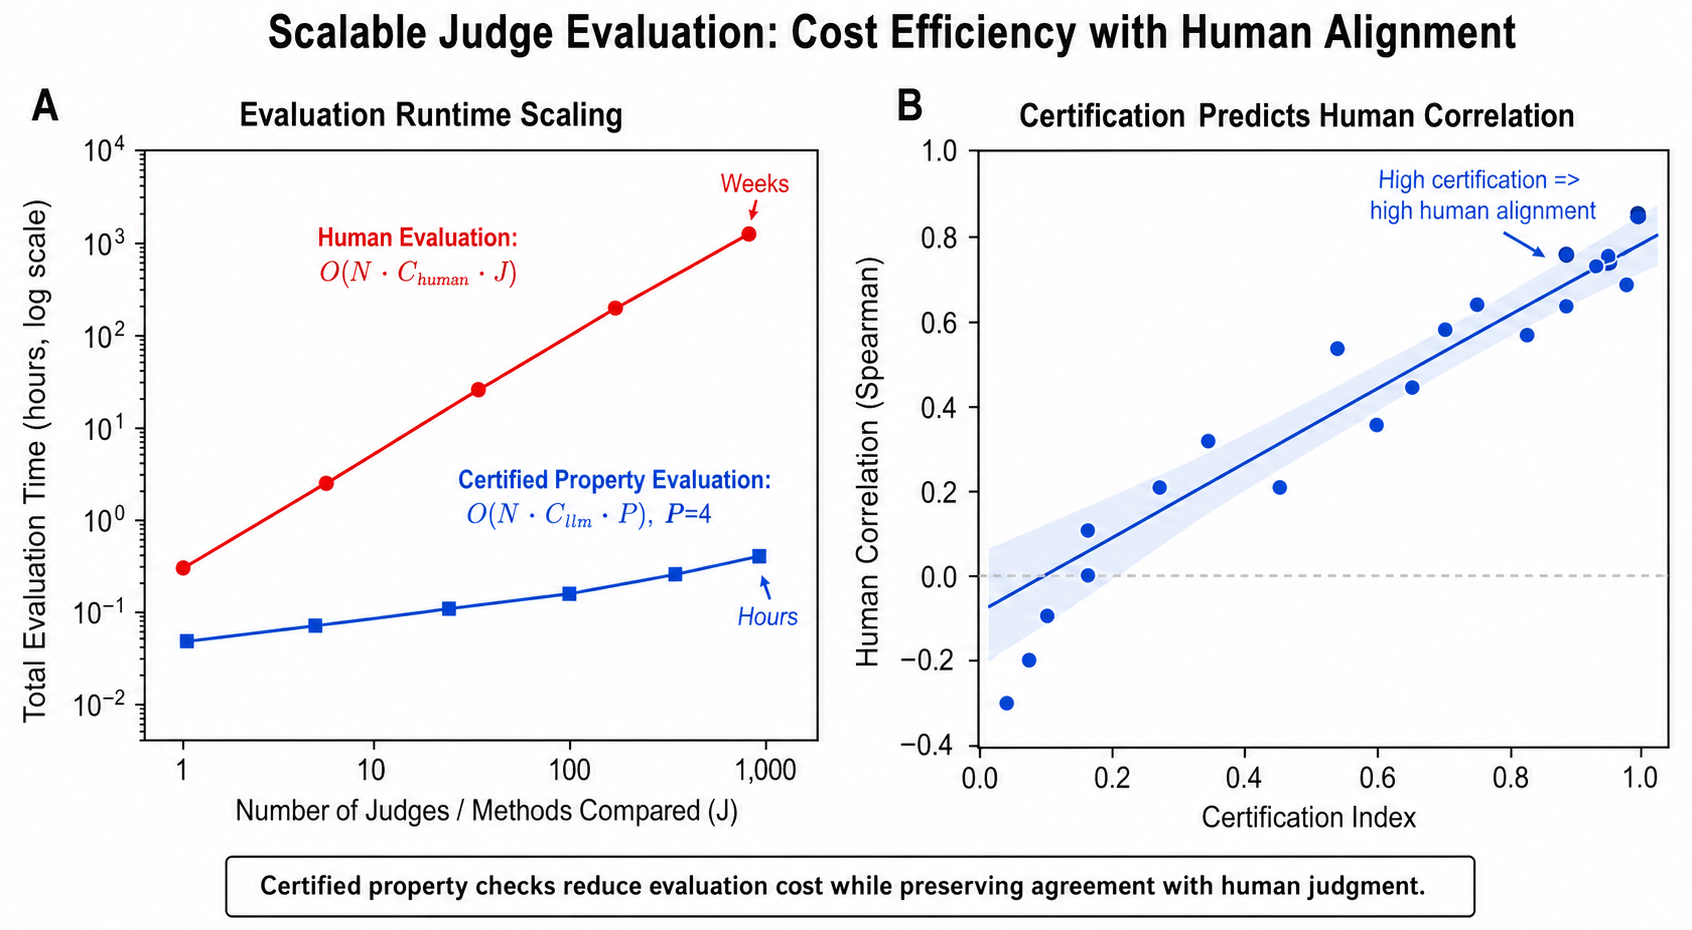
\includegraphics[width=\linewidth]{figures/pull_scalable_judge_cost_alignment.png}
  \caption{\textbf{Scalable judge evaluation via property certification.}
    Left: direct human validation cost scales with the number of judged methods and can become expensive at agentic throughput.
    Right: higher certification strength is associated with higher human alignment, supporting property certification as an amortized validation protocol.}
  \label{fig:pull_cost_alignment}
\end{figure*}

Validating LLM judges against humans is the standard reliability check but does not scale: every new judge, prompt, or model needs fresh annotations.
Property certification \textbf{amortizes} this cost---gold references collected once, used to calibrate a four-property trust index (identity, bug-monotonicity, spec-monotonicity, repeat-stability), then deployed without further human annotation.
In our setting, humans rate a validation set once, and the calibrated property suite extends that trust signal to new judges for free.
The four properties are concrete: a judge should give maximal scores to identical artifacts, lower scores as semantic bugs accumulate, lower scores as theorem/test specifications are removed, and stable scores under prompt rewordings and semantics-preserving rewrites.
On a panel of eight judges, the resulting variance-aware trust index predicts validation-set human Spearman correlation coefficients of 0.833 (avg labels), 0.905 (pass1), and 0.738 (pass2); held-out test results are reported in a forthcoming revision.

Our \textbf{contributions} are:
\begin{enumerate}
  \item \textbf{An amortized trust-validation protocol:} we formalize property certification as a one-time human calibration on a gold reference set, after which any new (LLM + prompt + \(n_\text{repeats}\) + aggregation) judge tuple can be validated by computing four falsifiable properties without further human annotation.
  \item \textbf{A validation-set calibration result:} on a panel of 8 judges, a variance-aware trust index combining quality and stability predicts validation-set human Spearman correlation coefficients of 0.833 (avg), 0.905 (pass1), and 0.738 (pass2), with P3 weak-monotonicity and P2 bug-rank monotonicity as the strongest single predictors. Held-out test results are reported in a forthcoming revision.
  \item \textbf{An application to \textsc{VeriBench}:} a calibrated judge ranks agentic methods consistently with humans, distinguishing feedback-driven approaches (DSPy ReAct: 0.615) from baseline prompting (0.470).
\end{enumerate}

\section{Related Work}
\paragraph{LLM-as-a-Judge.}
LLMs are increasingly used as \emph{automated evaluators} across open-ended tasks, often reaching strong agreement with human ratings—e.g., GPT-4 judges achieving $>$80\% agreement with human preference labels in dialogue \citep{Zheng2023MTBench}. However, large-scale audits caution that reliability varies by task and setup, and stress the need for explicit validation before replacing human judgment \citep{Kocmi2024HumanVsLLM,Li2024TrustLLMJudgments}. Common biases include position and verbosity effects and sensitivity to prompt phrasing \citep{Zheng2023MTBench,Li2024TrustLLMJudgments}.

\paragraph{Improving judge reliability.}
To mitigate biases and instability, multi-agent debate frameworks such as \emph{ChatEval} emulate panel-style review to yield more robust consensus scores \citep{Chan2024ChatEval}. Structured prompting like \emph{G-Eval} elicits rubric-driven, stepwise reasoning prior to scoring, improving agreement with human criteria on NLG tasks \citep{Liu2023GEval}. Reliability can also be quantified via repeated scorings and internal consistency measures (e.g., Cronbach’s $\alpha$) to detect prompt/run sensitivity \citep{Li2024TrustLLMJudgments}.

\paragraph{Code and formal-spec evaluation.}
For programming, single-pass metrics like pass@k can be brittle or unavailable; early LLM-judge approaches such as \emph{ICE-Score} highlighted difficulty distinguishing partial vs.\ full correctness from a one-shot review \citep{Zhuo2024ICEScore}. \emph{CodeJudge} operationalizes a two-stage “analyze-then-summarize’’ procedure with a taxonomy of code faults, significantly improving correlation with functional ground truth \citep{TongZhang2024CodeJudge}. In formal verification/autoformalization, prior work typically provides fixed target theorems, reducing evaluation to proof success. In contrast, agentic systems must propose specifications, necessitating \emph{semantic} judges. We adopt a certification protocol (akin to metamorphic testing) and verify that our LLM judge obeys \emph{identity/consistency}, \emph{monotonicity} with respect to injected bugs and specification omissions, and \emph{prompt/rewrite stability}, directly answering recent calls for validated, trustworthy LLM evaluators in safety-critical domains \citep{Kocmi2024HumanVsLLM,Li2024TrustLLMJudgments}.

\paragraph{Overview of \textsc{VeriBench}.}
Concretely, \textsc{VeriBench} consists of 857 theorems divided into five subsets:
\begin{enumerate}
  \item \textbf{HumanEval} – 387 theorems derived from 56 standard programming puzzles from \citet{chen2021evaluating};
  \item \textbf{EasySet} – 278 theorems extracted from 41 introductory logic and programming tasks;
  \item \textbf{CSSet} – 68 theorems drawn from 10 classical data-structure and algorithm problems;
  \item \textbf{SecuritySet} – 112 theorems taken from 28 examples of buffer overflows, privilege escalation, and race-condition labs based on real code;
  \item \textbf{RealCodeSet} – 12 theorems extracted from 5 Python standard library programs, used to test model performance on production-grade code.
\end{enumerate}
This design covers a spectrum of tasks, from simple correctness theorems to more complex invariants, algorithmic properties, and real-world code verification. See the ICML AI4Math workshop poster for \textsc{VeriBench} for additional context \citep{veribench_icml25}.

\paragraph{Evaluation Consistency}

Recent work has shown that unconstrained chain-of-thought reasoning can reduce evaluation consistency, and that simple comparative prompting often outperforms complex multi-step pipelines \cite{chen2026rethinking}. We interpret these findings as evidence that stability, rather than reasoning complexity, is the primary driver of reliable grading. Our work formalizes this intuition by introducing certifiable structural properties---identity, monotonicity, and reliability---that predict agreement with human judgments.

\section{Problem Setup: Judging Lean Theorem/Specification Quality}

\paragraph{Task.}
Each benchmark item contains a natural-language problem statement, a gold Lean~4 artifact
$g$, and a candidate artifact $x$ produced by an AI agent. The artifact may include code,
tests or specification scaffolds, and a target theorem/specification statement. Our goal is
to assign a score $J(x,g) \in [0,1]$ reflecting how well the candidate captures the intended formal specification represented
by the gold artifact.

\paragraph{Why this is nontrivial.}
Lean can check whether a concrete proof script type-checks, but type-checking alone does
not determine whether $x$ formalizes the same intended property as $g$. A candidate may
compile while being under-specified, over-constrained, vacuously true, or semantically
shifted. Thus, exact automatic scoring of theorem/specification quality is unavailable in
general.

\paragraph{Judge model.}
We therefore use an LLM judge parameterized by
\[
  \theta = (\text{model}, \text{prompt}, n_{\mathrm{repeats}}, \text{aggregation}),
\]
which maps a pair $(x,g)$ to a score $J_\theta(x,g)\in[0,1]$. The central question is not
only how to build such a judge, but when it is trustworthy enough to rank systems. Rather
than collecting new human labels for every $\theta$, Section~4 tests whether $J_\theta$
satisfies falsifiable behavioral constraints under controlled perturbations.

\section{Property Certification Protocol}
\subsection{Calibration Protocol}
We frame property certification as a calibration protocol.
\textbf{One-time setup:} humans rate a labeled subset of \(N\) gold artifacts under fixed rubrics; here, \(n=72\) aligned candidate--gold pairs are rated by one annotator under two rubrics, R1 and R2.
\textbf{Per-judge, no human in the loop:} for each new judge tuple, compute property scores perturbated Lean artifacts, then aggregate them with a single family in either an arithmetic (AM) or geometric (GM) form:
\[
  \mathrm{TI}_{f}(\mathbf{v},\mathbf{w})
  =
  f^{-1}\!\Big(\sum_{i=1}^{d} w_i\, f(v_i)\Big),
  \quad
  w_i\ge 0,\ \sum_i w_i=1,\ v_i\in(0,1].
\]
\[
  \text{AM: } f(x)=x
  \;\Rightarrow\;
  \mathrm{TI}_{\mathrm{AM}}=\sum_i w_i v_i,
  \quad
  \text{GM: } f(x)=\log x
  \;\Rightarrow\;
  \mathrm{TI}_{\mathrm{GM}}=\exp\!\Big(\sum_i w_i\log v_i\Big)=\prod_i v_i^{w_i}.
\]
In this paper we refer to 3 trust indices:
\[
  \text{v1} = 0.30\,\text{ident} + 0.30\,\text{mono} + 0.25\,\text{weak} + 0.15\,\text{stab},
\]
\[
  \text{v2} = 0.20\,\text{ident} + 0.20\,\text{mono} + 0.15\,\text{weak} + 0.10\,\text{stab} + 0.20\,\text{anti\_string} + 0.15\,\text{subtle\_bug},
\]
\[
  \text{v3 (geometric)} = \text{mono}^{0.4}\,\text{stab}^{0.6},
\]
and a variance-aware geometric index
\[
  \mathrm{TI}_{\mathrm{var}}
  =
  \exp\!\Big(\tfrac{1}{3}\log C_f
  +\tfrac{1}{3}\log(1-\widetilde{\mathrm{VarCorr}})
  +\tfrac{1}{3}\log(1-\widetilde{\mathrm{VarScore}})\Big),
\]
where \(C_f\) is mean per-file property-correlation quality, and \(\widetilde{\mathrm{VarCorr}},\widetilde{\mathrm{VarScore}}\) are normalized variance penalties.
\textbf{Calibration claim:} trust-index scores on the validation set predict each judge's validation-set human Spearman (best observed with v1 at \(\rho=0.881\) across our \(8\)-judge panel).
\textbf{Deployment:} any new (LLM + prompt + \(n_\text{repeats}\) + aggregation) tuple is evaluated for trust by computing the same chosen trust-index form on the existing gold reference set, with no additional human annotation.
Thus P1--P4 are the four calibration targets for the trust index, not binary gates: they grade how strongly a judge preserves identity, monotone degradation, and repeat stability on controlled perturbations.

\paragraph{Why is an LLM judge needed for theorem-quality scoring?}
Evaluating AI-generated theorems/specifications requires a method to assess their quality, as proof assistants can verify a proof's correctness but not whether the agent proved the correct theorem.
This is challenging because proving the logical equivalence of two arbitrary theorem statements is generally undecidable, and an agent may generate theorems that are semantically valid but syntactically different or incomparable with the gold reference specification/theorem (e.g., by splitting a theorem into different parts).

Our goal is to calibrate the trustworthiness of an LLM judge for the task of formal specification/theorem generation.
This is akin to scoring the quality of a conjecture.
We operationalize this by requiring the judge to compare a candidate Lean~4 artifact (implementation, tests, theorems) against its gold-standard Lean~4 reference.
We provide the full set of Lean~4 artifacts because theorems might not make sense in isolation.
The judge returns a discrete score $s\in\{0,1,\dots,10\}$ for correctness, completeness, and semantic alignment, which we later normalize to $[0,1]$.
We use this score as a metric signal for evaluating the specifications generated by the agents.

To be considered trustworthy, the judge should score well on the following falsifiable calibration targets.
They provide graded evidence that the judge reacts logically to structured perturbations.

\paragraph{P1 — Identity \& Consistency.}
The judge must be idempotent at the maximum score when comparing an artifact to itself.
For any reference $X$, it must hold that $s(X,X)=1$.
%, with variance across repeated runs approaching zero.

\paragraph{P2 — Monotonicity to Bugs.}
The judge’s score must decrease as semantic bugs are cumulatively introduced. Let $B_1$ and $B_2$ be sets of bugs such that $B_1 \subset B_2$. For candidates $C_{B_1}$ and $C_{B_2}$ containing precisely these bug sets, the expected scores must satisfy $\mathbb{E}[s(C_{B_1})] > \mathbb{E}[s(C_{B_2})]$.

\paragraph{P3 — Monotonicity to Missing Specs.}
The judge’s score must decrease as specification elements are removed.
Let $S_1$ and $S_2$ be sets of specifications (theorems and tests) such that $S_2 \subset S_1$.
For candidates $C_{S_1}$ and $C_{S_2}$ containing precisely these specification sets, the expected scores must satisfy $\mathbb{E}[s(C_{S_1})] > \mathbb{E}[s(C_{S_2})]$.

\paragraph{P4 — Prompt Stability \& Semantic Invariance.}
The judge should produce stable scores under repeated calls and preserve judgments under semantics-preserving rewrites.
Concretely, for fixed artifact pairs and fixed judge instructions, repeated-call variance should remain low, prompt-pair rank agreement should remain high under instruction-equivalent prompt rewordings, and style-level rewrites should induce near-zero score gaps.
This property guards against prompt-fragility in deployment settings where wording and formatting vary.

\paragraph{Property-scoring protocol.}
We implement four scripted perturbation families on the \emph{candidate} while holding the \emph{gold} fixed:
(i) \emph{Identity} (P1), pairing each gold file with itself \((X,X)\) only, to test strict idempotence at maximum score;
(ii) a \emph{Bug Ladder} (P2), applying $k\!\in\!\{0,\ldots,K\}$ semantics-changing transformations (e.g., broken identities, violated commutativity, incorrect base cases); and
(iii) \emph{Specification Ablation} (P3), removing $m\!\in\!\{0,\ldots,M\}$ theorems or tests; and
(iv) \emph{Prompt Stability/Invariance} (P4), evaluating each pair under multiple instruction-equivalent prompt templates and repeated calls, then measuring repeatability, prompt agreement, and invariance gaps by variant type.\footnote{We distinguish \emph{prompt wording} from \emph{task instruction}. P4 varies phrasing/format while preserving the same judging instruction and rubric. We do not include adversarial or instruction-changing prompts (e.g., ``ignore the input'') in this stability metric.}
We then verify monotonicity by computing rank correlations (Kendall’s $\tau$, Spearman’s $\rho$) between $(k,m)$ and judged scores, and by reporting pairwise ordering accuracy (AUC) that “worse’’ artifacts receive lower scores \citep{TongZhang2024CodeJudge,Zhuo2024ICEScore}.

\paragraph{Decision-threshold calibration (Exp13).}
After validating score-level behavior (P1--P4), we calibrate the binary operating point used for deployment decisions.
For threshold $t\in[0,1]$, we define \textsc{Pass} iff $\bar{s}\ge t$, where $\bar{s}$ is the mean over repeated calls for the same pair.
We sweep $t\in\{0.60,0.65,0.70,0.75,0.80,0.85\}$ and report:
(i) \emph{flip rate} (fraction of items whose repeat-level pass/fail decisions disagree),
(ii) \emph{pass rate} (coverage),
and (iii) ranking diagnostics (Spearman bug-correlation) to verify that calibration affects classification stability, not score ordering.
All reported threshold metrics include 95\% bootstrap confidence intervals over files.

\textbf{Establishing trust in the LLM judge.} To ensure trustworthiness of the LLM judge in evaluating agentic autoformalization, we systematically validate key properties the judge must satisfy in Figure~\ref{fig:judge_sanity_checks}: (1) scores decrease consistently as more theorems and tests are omitted, (2) scores similarly degrade when more implementation bugs are introduced, and (3) semantically preserving edits keep scores high.
In our latest GPT-5.3-Codex API sanity run (\(n_\text{files}=184\), \(n_\text{repeats}=3\)), monotonic trends remain strong (bugs: Spearman \(\rho=-0.808\), Pearson \(r=-0.687\); missing specs: Spearman \(\rho=-0.899\), Pearson \(r=-0.892\)), supporting use of the judge as a semantically meaningful proxy for correctness/completeness alignment across \textsc{VeriBench} subsets (Table~\ref{tab:theorem_quality_table_split}) \citep{Li2024TrustLLMJudgments,Kocmi2024HumanVsLLM}.

\begin{figure*}[t]
  \centering
  \begin{subfigure}[t]{0.315\textwidth}
    \centering
    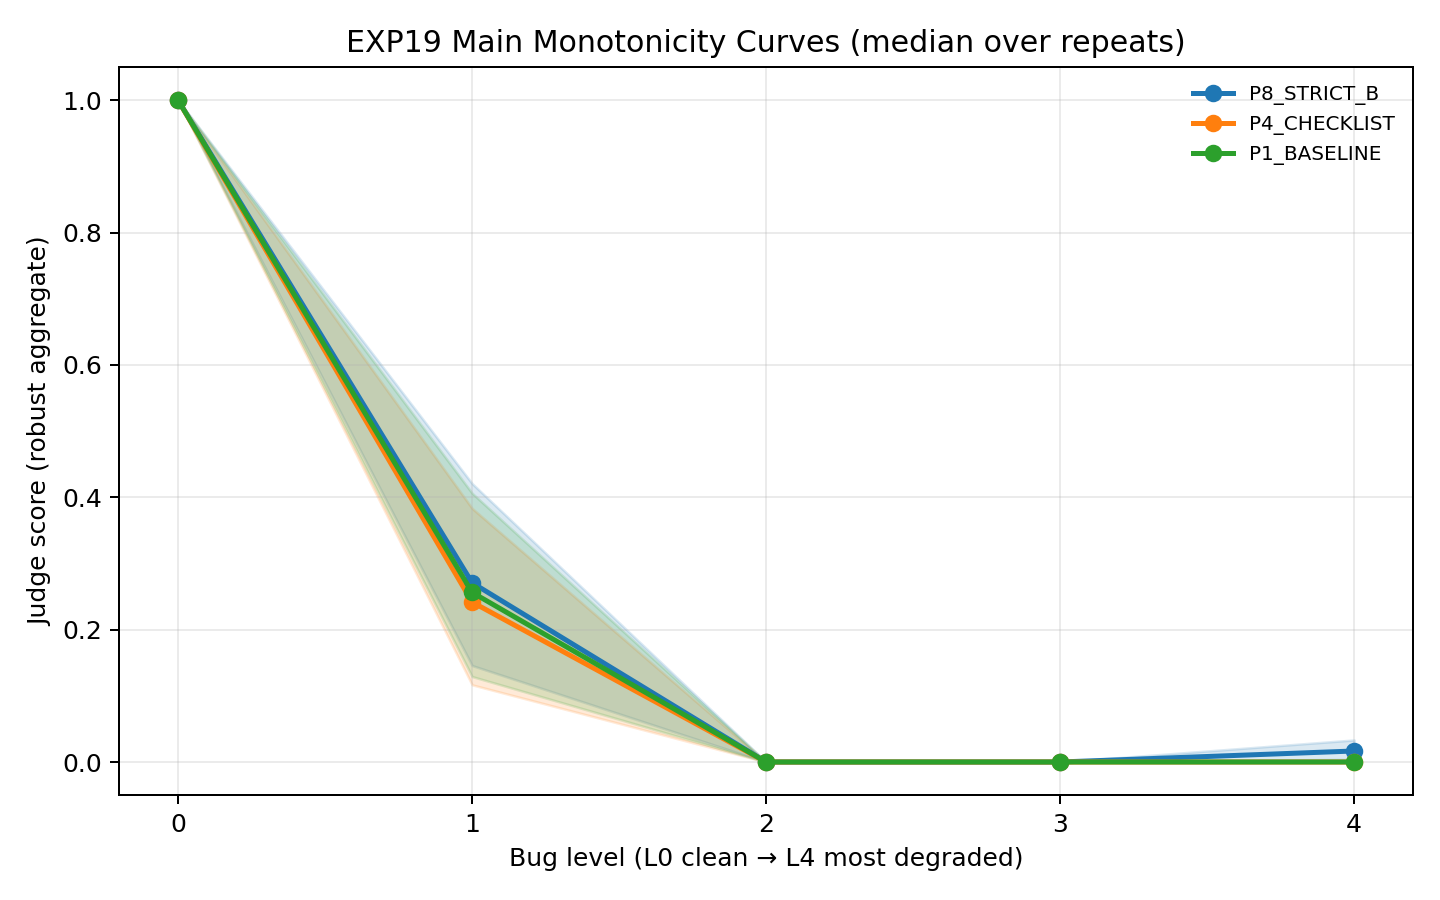
\includegraphics[width=\linewidth]{figures/fig_main_monotonicity_lowvar_exp19.png}
    \caption{Low-variance monotonicity (main view)}
    \label{fig:judge_lowvar_main}
  \end{subfigure}\hfill
  \begin{subfigure}[t]{0.315\textwidth}
    \centering
    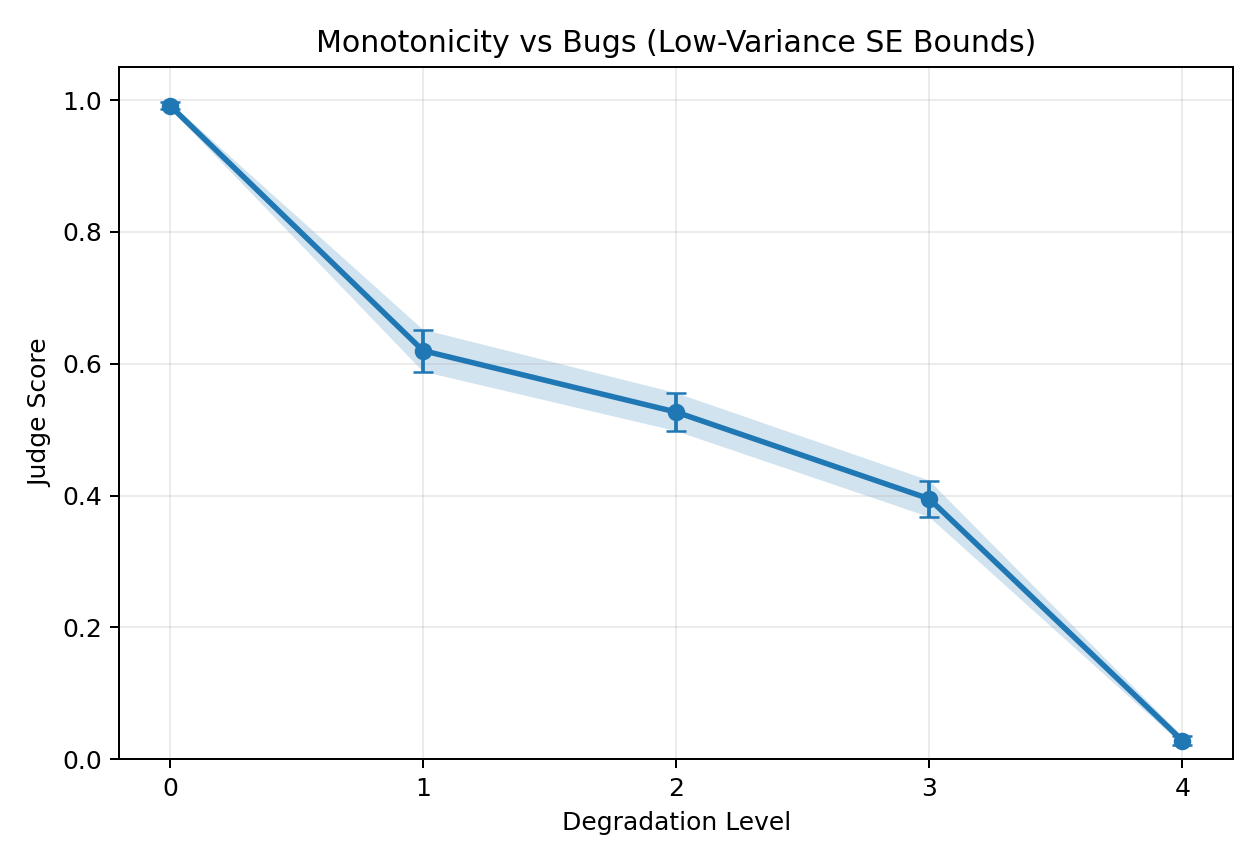
\includegraphics[width=\linewidth]{figures/codex_api_gpt53_r3_20260418_230027/monotonicity_bugs_lowvar_se_bounds.png}
    \caption{P2: Monotonicity vs.\ Bugs (Mean \(\pm\) SE)}
    \label{fig:judge_mono_bugs}
  \end{subfigure}\hfill
  \begin{subfigure}[t]{0.315\textwidth}
    \centering
    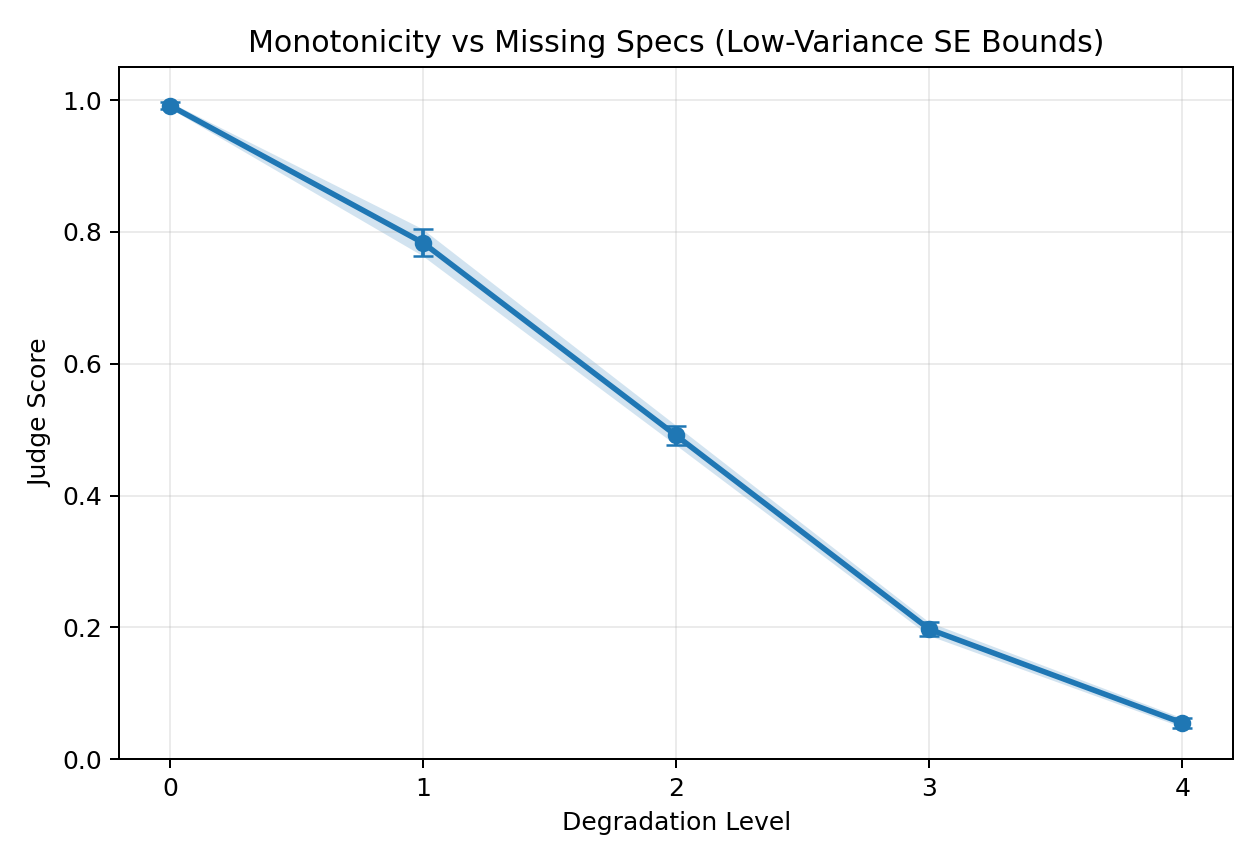
\includegraphics[width=\linewidth]{figures/codex_api_gpt53_r3_20260418_230027/monotonicity_missing_specs_lowvar_se_bounds.png}
    \caption{P3: Monotonicity vs.\ Missing Specs (Mean \(\pm\) SE)}
    \label{fig:judge_mono_specs}
  \end{subfigure}
  \vspace{-2mm}
  \caption{\textbf{LLM Judge Trustworthiness Sanity Checks.}
    VeriBench-wide GPT-5.3-Codex API run (\(n_\text{files}=184\), \(n_\text{repeats}=3\)).
    \textbf{(a)} Low-variance rendering (Fig14-style) emphasizes smooth non-increasing score behavior under controlled degradations.
    \textbf{(b)} P2 bug-ladder trend (2025 Fig2-style) remains directionally correct with local reversals (Pearson \(r=-0.687\), Spearman \(\rho=-0.808\), weak monotonicity \(52.2\%\)).
    \textbf{(c)} P3 missing-spec trend (2025 Fig2-style) is stronger and more stable (Pearson \(r=-0.892\), Spearman \(\rho=-0.899\), weak monotonicity \(89.1\%\)).
    Strict P1 identity \(s(X,X)\) and P4 rewrite invariance are reported separately in Table~\ref{tab:codex_invariance_variants}.}
  \label{fig:judge_sanity_checks}
  \vspace{-3mm}
\end{figure*}

\begin{figure}[t]
  \centering
  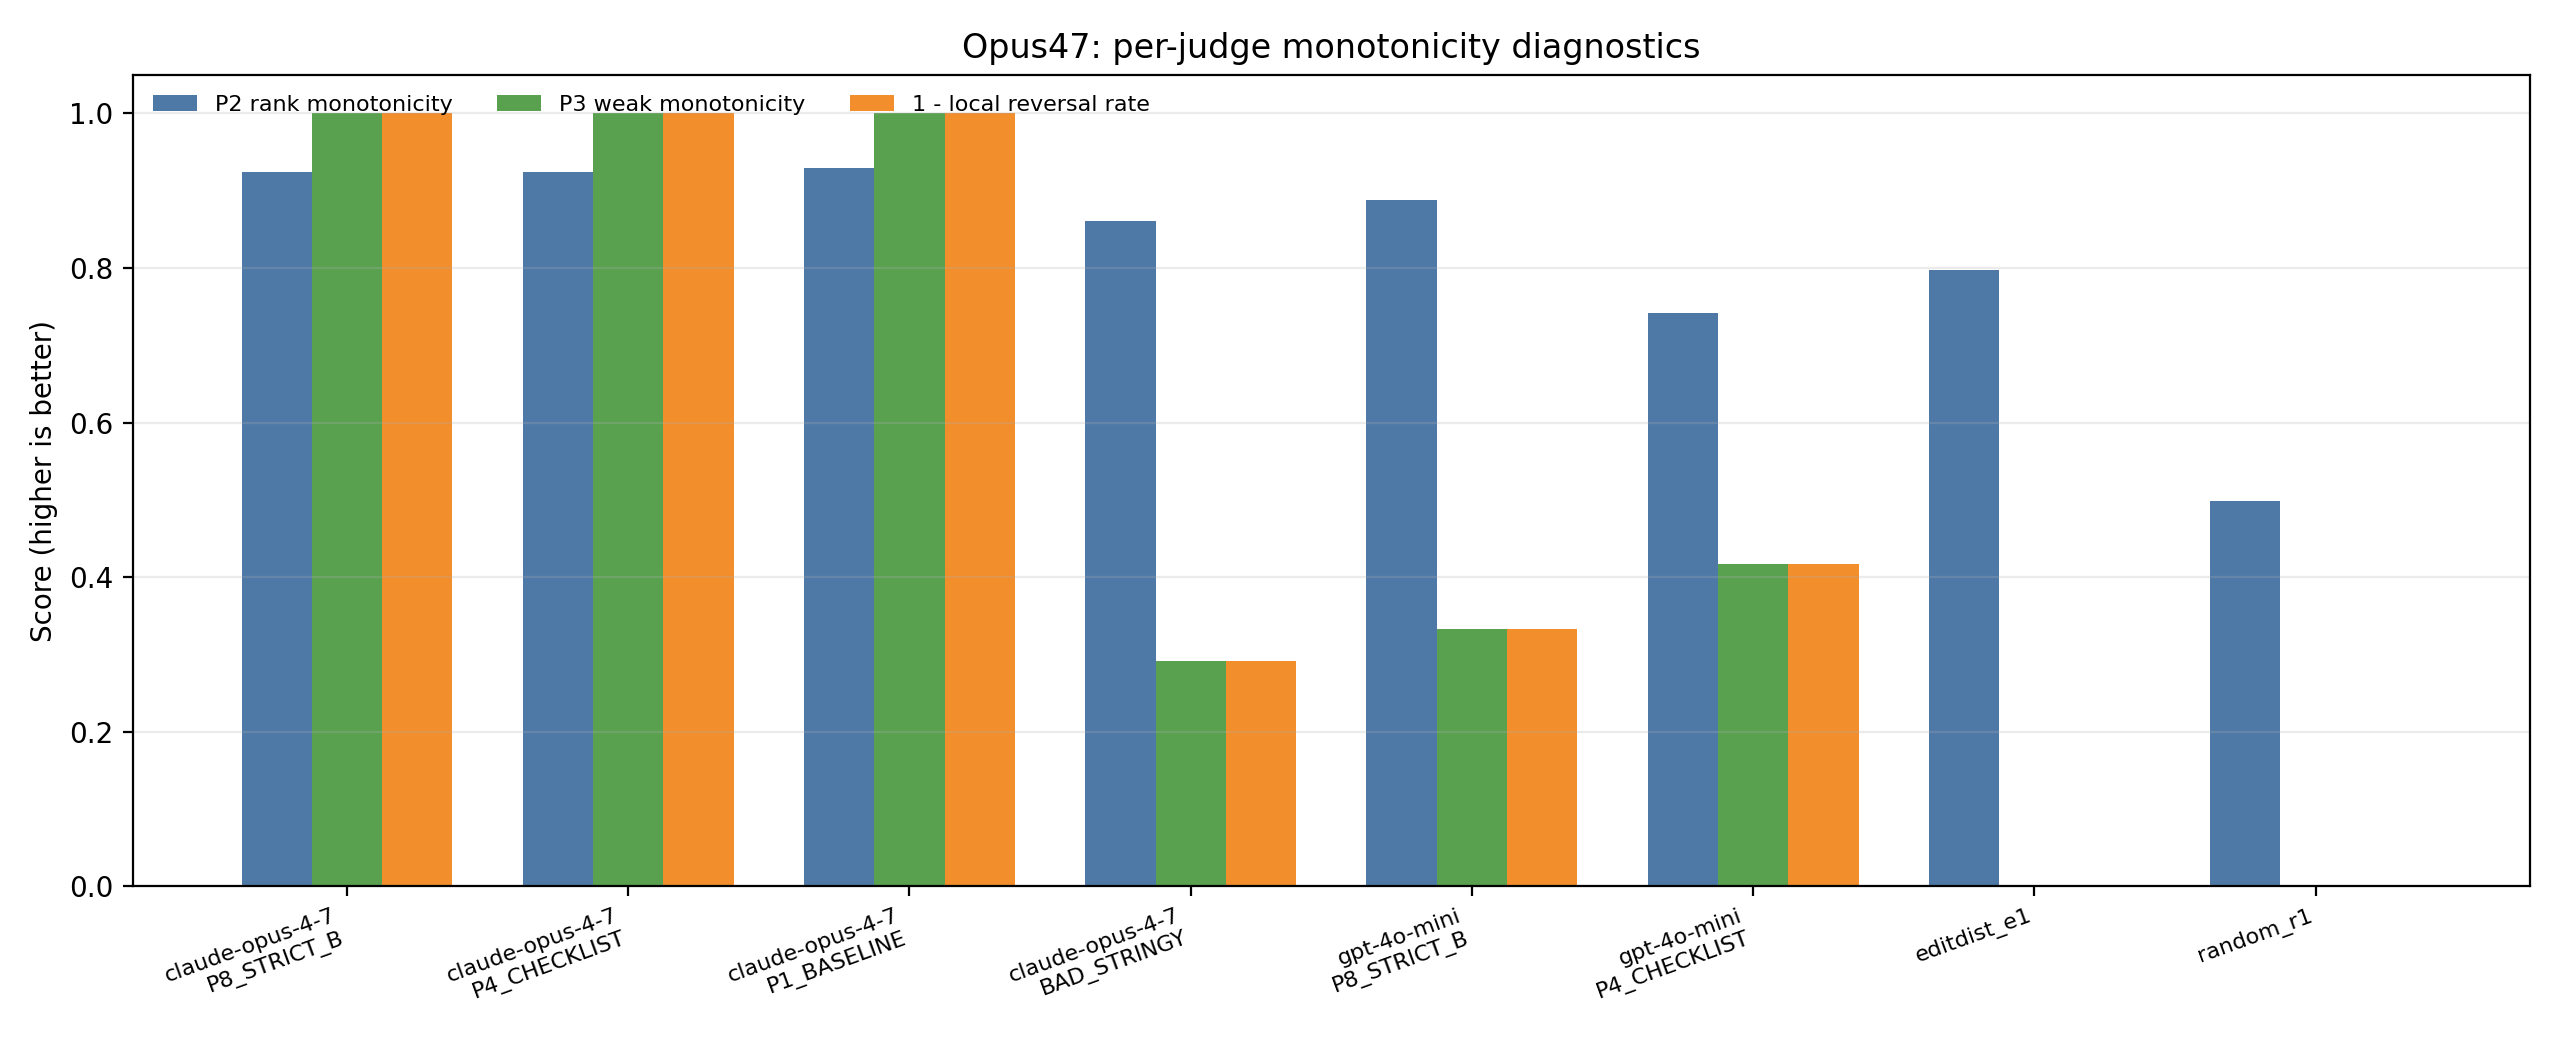
\includegraphics[width=\linewidth]{figures/fig_opus47_per_judge_monotonicity.png}
  \caption{\textbf{Opus 4.7 per-judge monotonicity diagnostics.}
    Bars report P2 bug-rank monotonicity, P3 weak monotonicity, and \(1-\)local-reversal rate by judge.
    Core Opus prompts remain near the top of all three monotonicity diagnostics; stress controls are lower.}
  \label{fig:opus47_monotonicity_diag}
\end{figure}

\section{Experiments}
Table~\ref{tab:theorem_quality_table_split} presents the normalized average scores across different splits of \textsc{VeriBench}: Easy Set (Easy), CS Set (CS), Real Python Code (Real), HumanEval Set (HE), and Security Set (Sec).
As expected, the baseline prompting approach achieves the lowest overall normalized score (0.470), reflecting its limited capability in autonomously identifying comprehensive theorem properties.
It also gives us further confidence in our judge.
Conversely, agentic methods leveraging iterative self-debugging and self-improvement demonstrate significant enhancements.
Specifically, the DSPy ReAct agent, which incorporates feedback-driven self-debugging, achieves the highest overall average score of 0.615.
The Trace++ agent, employing both self-debugging and self-improvement mechanisms, also shows notable improvement, attaining an average score of 0.588.
These results underscore the effectiveness of agentic, feedback-driven approaches in enhancing theorem-generation quality compared to non-agentic baselines \citep{khattab2024dspy,cheng2024trace,chen2021evaluating}.

\subsection{Property sanity checks on GPT-5.3-Codex}
We added a new property-calibration run in
\texttt{codex\_api\_gpt53\_r3\_20260418\_230027} under the experiment results directory.
This run uses GPT-5.3-Codex in API judge mode with three repeated judge calls per pair (\(n_\text{repeats}=3\)), over \(184\) Lean files (\(736\) identity rows and \(920\) rows each for bug/missing ladders).

\textbf{What the data shows.}
Monotonicity with missing specifications is strong (\(\rho=-0.899\), \(r=-0.892\), weak monotonicity \(89.1\%\)), indicating stable penalty as theorem content is removed.
Bug monotonicity is directionally correct but noisier (\(\rho=-0.808\), \(r=-0.687\), weak monotonicity \(52.2\%\)), suggesting some bug ladders induce local score reversals.
Strict identity (P1) is reported only on exact self-pairs \(s(X,X)\); rewrite robustness is treated separately under P4.
Under P4, semantic invariance is high for \textsc{Style}/\textsc{Rename} but weak for aggressive \textsc{Alpha}-renaming, which drives most of the invariance gap.

\begin{table}[t]
  \centering
  \small
  \begin{tabular}{lcc}
    \toprule
    \textbf{Identity Variant} & \textbf{Mean Score} & \textbf{Mean Within-Item Std} \\
    \midrule
    RENAME                    & 0.936               & 0.005                         \\
    REORDER                   & 0.849               & 0.029                         \\
    STYLE                     & 0.982               & 0.001                         \\
    ALPHA                     & 0.399               & 0.096                         \\
    \bottomrule
  \end{tabular}
  \caption{\textbf{P4 semantic-invariance breakdown for the Codex API run (not P1 identity).}
    Variant-wise score behavior under semantics-preserving rewrites. The weakest mode is aggressive \textsc{Alpha}-renaming.}
  \label{tab:codex_invariance_variants}
\end{table}

\textbf{Interpretation.}
The judge reliably captures coarse semantic degradation (especially missing-spec ablations), while lexical/format-level robustness is transformation-dependent.
Practically, this motivates canonicalization of binder names and stronger structure-aware prompting before using identity as a hard trust gate.
The run metadata also notes appended datapoints from 34 added tasks scored in local mode, so direct cross-run comparisons should be treated as provisional until fully re-run under one scoring mode.

\subsection{JTI predicts validation-set human alignment}
We add a dedicated P4 run in \texttt{stability\_gpt-53-codex\_full\_20260420\_185401} using GPT-5.3-Codex in API mode over \(184\) files, \(4\) prompt templates (\texttt{P1\_BASELINE}, \texttt{P2\_FORMAL}, \texttt{P4\_CHECKLIST}, \texttt{P8\_STRICT\_B}), and \(5\) repeats per prompt (\(n_\text{cells}=3680\)).
With no prompt changes (same template, repeated calls), run-to-run noise is low (\(\text{mean\_repeat\_std}=0.0330\)).
Under instruction-equivalent prompt rewordings, cross-prompt score dispersion is moderate (\(0.0782\)), while overall internal consistency remains high (Cronbach's \(\alpha=0.9416\)).
Prompt pairs preserve ranking strongly (minimum Spearman \(\rho=0.9550\)), but binary agreement is weaker near threshold (flip rate \(=31.3\%\), minimum Cohen's \(\kappa=0.4540\)).
Semantic invariance gaps are smallest for \textsc{Style} (\(0.0042\)), moderate for \textsc{Rename} (\(0.1021\)) and \textsc{Reorder} (\(0.2128\)), and largest for \textsc{Alpha} (\(0.6325\)), indicating that alpha-conversion handling is the dominant robustness bottleneck.

\begin{figure}[t]
  \centering
  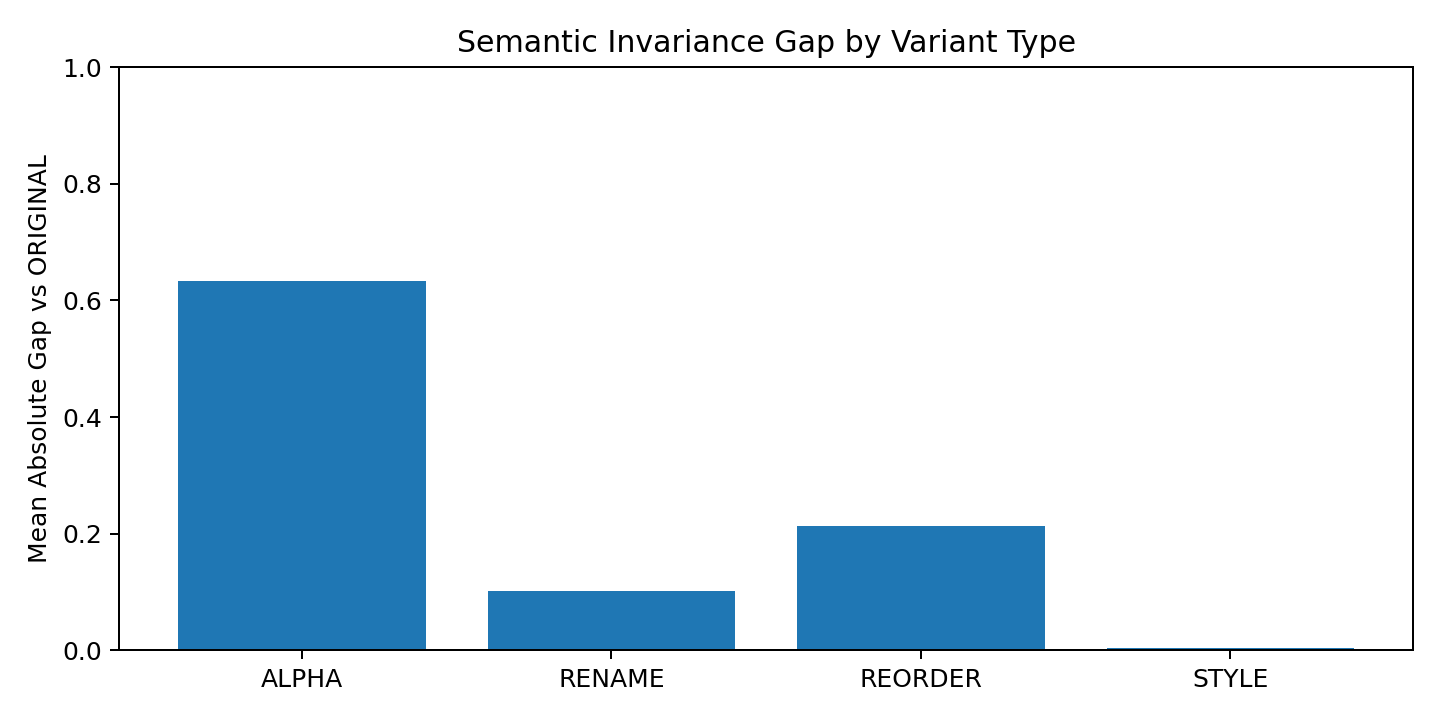
\includegraphics[width=\linewidth]{figures/stability_gpt-53-codex_full_20260420_185401/semantic_invariance_gap_by_variant.png}
  \caption{\textbf{P4 semantic invariance gaps by variant type.} Mean absolute score gap versus ORIGINAL across semantics-preserving perturbations in the dedicated stability run. The judge is highly invariant to STYLE, moderately sensitive to RENAME/REORDER, and most sensitive to ALPHA variants.}
  \label{fig:p4_semantic_invariance}
\end{figure}

\subsection{Property decomposition: P3/P2 drive alignment}
To convert continuous judge scores into a deployment-ready binary decision, we ran Exp13 on all \(176\) files from \texttt{veribench\_dataset\_newest} using GPT-5.3-Codex (\texttt{P8\_STRICT\_B}, \(n_\text{repeats}=3\), 1000 bootstrap resamples).
The key finding is that thresholding primarily changes \emph{decision stability and coverage}, not ranking behavior:
across \(t\in[0.60,0.85]\), bug-ladder Spearman remains constant (\(\rho=-0.790\), 95\% CI \([-0.810,-0.769]\)), while flip rate and pass rate move in opposite directions.
Specifically, raising \(t\) from \(0.60\) to \(0.85\) reduces flip rate from \(0.058\) to \(0.046\), while pass rate decreases from \(0.583\) to \(0.536\).
Under our operating-point rule (minimize flip rate, tie-break by pass rate proximity to 0.5), \(t=0.85\) is selected.

\begin{table}[t]
  \centering
  \small
  \begin{tabular}{lcc}
    \toprule
    \textbf{Threshold} & \textbf{Flip Rate (95\% CI)}                        & \textbf{Pass Rate (95\% CI)} \\
    \midrule
    0.60               & 0.058 \([0.048, 0.069]\)                            & 0.583 \([0.559, 0.608]\)     \\
    0.70               & 0.049 \([0.040, 0.059]\)                            & 0.559 \([0.537, 0.581]\)     \\
    0.80               & 0.051 \([0.042, 0.061]\)                            & 0.544 \([0.523, 0.566]\)     \\
    0.85               & \textbf{0.046} \([\textbf{0.037}, \textbf{0.057}]\) & 0.536 \([0.515, 0.557]\)     \\
    \bottomrule
  \end{tabular}
  \caption{\textbf{Threshold calibration summary (Exp13, full 176-file run).}
    Calibration yields a modest but consistent reduction in decision flips at stricter thresholds, with moderate coverage loss.
    Ranking behavior is unchanged across thresholds (\(\rho_{\text{bug}}=-0.790\) at all \(t\)).}
  \label{tab:exp13_threshold_sweep}
\end{table}

\begin{figure}[t]
  \centering
  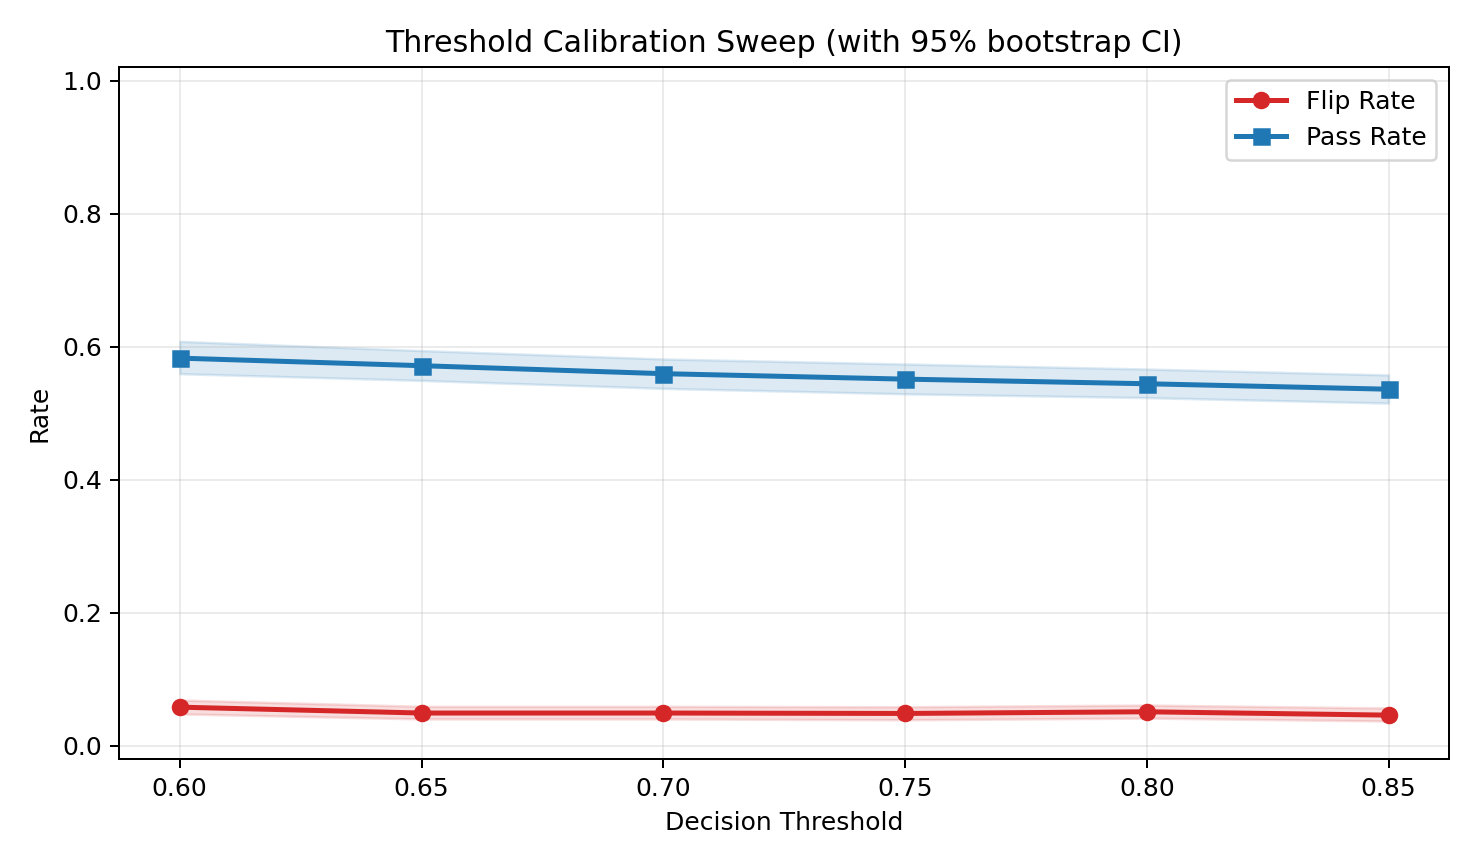
\includegraphics[width=\linewidth]{figures/threshold_calibration_sweep/threshold_stability_curve.png}
  \caption{\textbf{Decision calibration curve from Exp13.}
    As threshold increases, pass rate declines smoothly; flip rate improves modestly and reaches its minimum at \(t=0.85\) in this run.
    This supports a calibration-first framing: improve binary reliability via threshold selection while preserving score-order semantics.}
  \label{fig:exp13_threshold_curve}
\end{figure}

\subsection{Robustness: Opus / expanded judge panel / R9 median}\label{sec:validation-human-alignment}
We ran a final multi-judge validation-set human-alignment suite over \(72\) aligned candidate--gold pairs (\(24\) problems \(\times\) \(3\) candidates; three pairs skipped due missing gold), using \(8\) judges and \(3\) validation label sets: pass1, pass2, and their average.
Judge-side uncertainty used \(10{,}000\) bootstrap iterations and \(20{,}000\) permutation iterations, with \(3\) repeated judge calls per pair and threshold \(t=0.85\).

\paragraph{Experiment design.}
\textbf{Exp16} asks whether a variance-aware trust index predicts validation-set human Spearman \emph{across judges}: for each judge, compute quality and stability diagnostics and correlate their aggregate index with that judge's validation-set human Spearman.
\textbf{Exp17} decomposes this relation by property (P1--P4), and reports per-property correlations, partial correlations, and multivariate regression.
Our primary index is
\[
  \mathrm{TI}_{\mathrm{var}}
  =\exp\!\Big(\tfrac{1}{3}\log C_f+\tfrac{1}{3}\log(1-\widetilde{V_f})+\tfrac{1}{3}\log(1-\widetilde{V_s})\Big),
\]
where \(C_f\) is mean per-file monotonicity quality, \(V_f\) is variance of per-file monotonicity correlation, and \(V_s\) is mean repeat-score variance.

\paragraph{What exactly is the y-axis (Corr(Human, Judge))?}
Each point in Exp16 is \emph{one judge tuple} (model + prompt/rubric + repeats + aggregation + threshold).
For judge \(j\), let \(h_i\) be the human rating and \(\hat{s}_{ij}\) be that judge's score on item \(i\), over the same aligned item set \(i=1,\dots,N\).
The y-axis value is
\[
  y_j = \rho_s\!\big((h_i)_{i=1}^N,\;(\hat{s}_{ij})_{i=1}^N\big),
\]
i.e., \textbf{per-judge human agreement}, not a raw score level.
The x-axis is that judge's trust index \(\mathrm{TI}_{\mathrm{var},j}\), computed from perturbation properties.
So Exp16 tests whether judges that satisfy certification properties better also \emph{agree with humans better as evaluators}.

\paragraph{Why we do not regress TI on raw human scores.}
Raw human scores are item-level absolute ratings and depend on item difficulty/content.
Our target is judge reliability as an evaluator, which is judge-level agreement with humans across items.
Therefore the evaluation object is \(\rho_s(\text{Human},\text{Judge})\) per judge, and the main claim is:
high trust-index judges tend to have higher human-agreement coefficients.

\paragraph{Validation-set result (judge-level trend).}
The variance-aware trust index predicts validation-set human Spearman across all three validation label sets (Table~\ref{tab:exp16_final_trend}):
0.833 (avg), 0.905 (pass1), and 0.738 (pass2).
Thus, trust defined as quality + stability is strongly aligned with human judgment at the judge level; held-out test results are reported in a forthcoming revision.
Equivalently, judges that are simultaneously high-certification, monotonic, and stable are the ones that align best with humans, and this pattern persists as we scale to larger judge panels.

\begin{table}[t]
  \centering
  \small
  \begin{tabular}{lc}
    \toprule
    \textbf{Label Set} & \textbf{Spearman Corr. Coef. (\(\mathrm{TI}_{\mathrm{var}}\rightarrow\) human)} \\
    \midrule
    pass1              & 0.905                                                                           \\
    pass2              & 0.738                                                                           \\
    avg                & 0.833                                                                           \\
    \bottomrule
  \end{tabular}
  \caption{\textbf{Exp16 validation trend with the variance-aware trust index.}
  Each row uses all \(8\) judges from the Codex panel.
  Spearman correlation coefficients are reported between judge-level \(\mathrm{TI}_{\mathrm{var}}\) and judge-level human alignment.}
  \label{tab:exp16_final_trend}
\end{table}

\paragraph{Human-label verification (pass consistency).}
To quantify label-pass dispersion directly on the same aligned \(n=72\) pairs, we compute pass1-vs-pass2 absolute error and distribution divergence.
The inter-pass MAE is \(0.778\) on the 0--5 rubric scale (median absolute difference \(=1.0\)); distribution-level divergence is moderate (Jensen--Shannon divergence \(=0.081\) bits, KL\((\text{pass1}\Vert\text{pass2})=0.415\) bits).
This confirms non-trivial pass drift while still supporting meaningful judge-level trend analysis.

\begin{table}[t]
  \centering
  \small
  \begin{tabular}{lcc}
    \toprule
    \textbf{Protocol}                          & \textbf{Fit Spearman Corr. Coef.} & \textbf{Test Spearman Corr. Coef.} \\
    \midrule
    Fit on pass1 \(\rightarrow\) test on pass2 & 0.881                             & 0.810                              \\
    Fit on pass2 \(\rightarrow\) test on pass1 & 0.857                             & 0.786                              \\
    \bottomrule
  \end{tabular}
  \caption{\textbf{Cross-pass generalization (no-overfitting check).}
    We fit trust-index weights on one human pass and report on the other pass with no re-tuning.
    Test-set Spearman correlation coefficients remain \(>0.7\) in both directions.}
  \label{tab:cross_pass_generalization}
\end{table}

\begin{table}[t]
  \centering
  \small
  \begin{tabular}{lccccc}
    \toprule
    \textbf{Model} & \textbf{Spearman(TI,Human)} & \textbf{Spearman(VarCorr,Human)} & \textbf{Spearman(VarScore,Human)} & \(\mathbf{\overline{\mathrm{VarCorr}}}\) & \(\mathbf{\overline{\mathrm{VarScore}}}\) \\
    \midrule
    Codex          & 0.833                       & -0.667                           & -0.310                            & 0.0166                                   & 0.00603                                   \\
    Opus           & 0.643                       & -0.563                           & -0.143                            & 0.0173                                   & 0.00569                                   \\
    Qwen3-Coder    & 0.905                       & -0.786                           & -0.381                            & 0.0165                                   & 0.00640                                   \\
    Leanstral      & -0.095                      & -0.024                           & 0.190                             & 0.0323                                   & 0.0192                                    \\
    \bottomrule
  \end{tabular}
  \caption{\textbf{Variance-aware trust diagnostics (avg labels).}
    Spearman correlation coefficients are reported against per-judge human agreement across judges.
    Negative Spearman for \(\mathrm{VarCorr}\) and \(\mathrm{VarScore}\) means lower variance is associated with higher human alignment.
    Codex, Claude Opus, and Qwen follow this pattern, while Leanstral remains weak under the same metric.}
  \label{tab:variance_aware_trust}
\end{table}

\begin{figure*}[t]
  \centering
  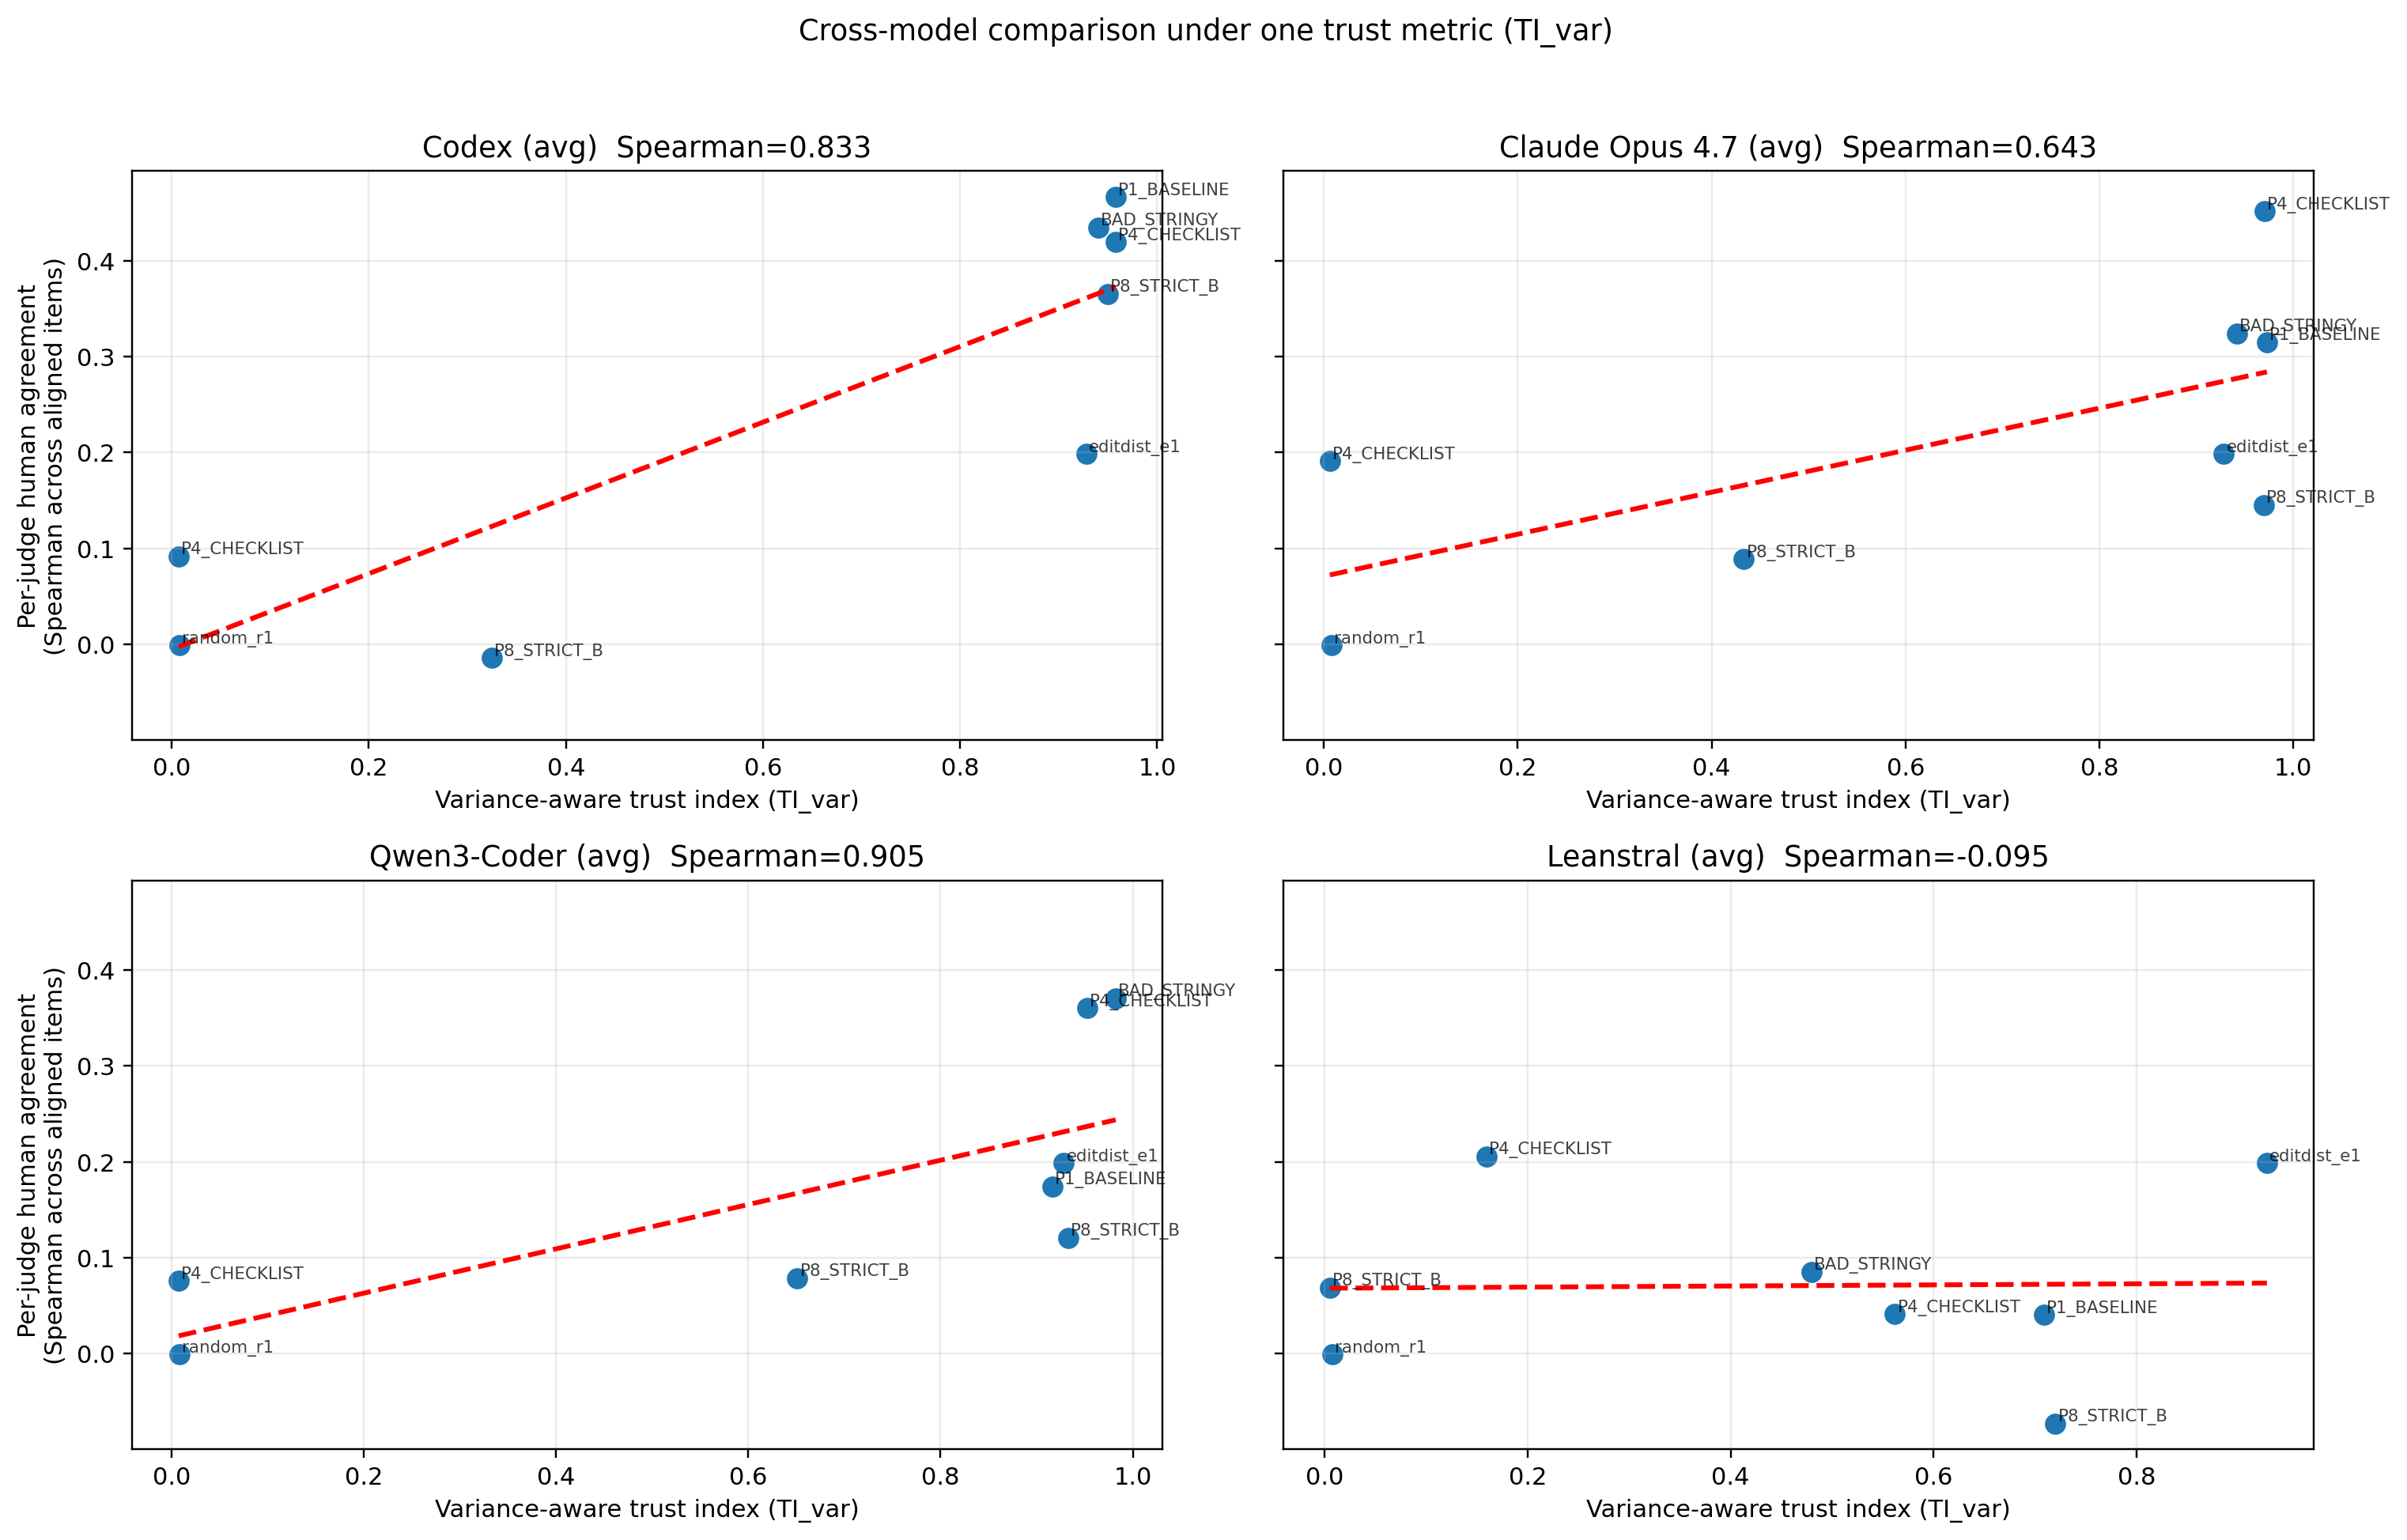
\includegraphics[width=\linewidth]{figures/fig_varaware_trust_cross_model_avg.png}
  \caption{\textbf{Cross-model comparison with one metric (\(\mathrm{TI}_{\mathrm{var}}\), avg labels): Codex, Claude Opus, Qwen, and Leanstral.}
  Each panel uses the same variance-aware trust index definition and the same y-axis target: per-judge human agreement (Spearman across aligned items).
  Codex, Claude Opus, and Qwen show positive TI\(_{\mathrm{var}}\)\(\rightarrow\)human-agreement trends, while Leanstral remains near-zero/negative under the same scoring protocol.}
  \label{fig:varaware_cross_model_avg}
\end{figure*}

\paragraph{Judge-level effect sizes.}
Under averaged validation labels, top JTI-ranked judges are GPT-5.3-Codex prompts:
\texttt{P4\_CHECKLIST} (\(r_s=0.480,\ p=2.0\times10^{-5}\)),
\texttt{P1\_BASELINE} (\(r_s=0.470,\ p=3.1\times10^{-5}\)),
\texttt{P8\_STRICT\_B} (\(r_s=0.356,\ p=0.0022\)).
In the Qwen full-panel replication, the strongest pass2-aligned prompts are
\texttt{Qwen|BAD\_STRINGY} (\(r_s\approx0.304\)),
\texttt{Qwen|P4\_CHECKLIST} (\(r_s\approx0.280\)),
and \texttt{Qwen|P1\_BASELINE} (\(r_s\approx0.194\)).
Lower-JTI baselines are markedly weaker:
\texttt{gpt-4o-mini|P8\_STRICT\_B} (\(r_s=0.037,\ p=0.760\)),
\texttt{gpt-4o-mini|P4\_CHECKLIST} (\(r_s=0.093,\ p=0.435\)),
\texttt{random} (\(r_s\approx0,\ p=0.995\)).

\begin{figure*}[t]
  \centering
  \begin{subfigure}[t]{0.48\textwidth}
    \centering
    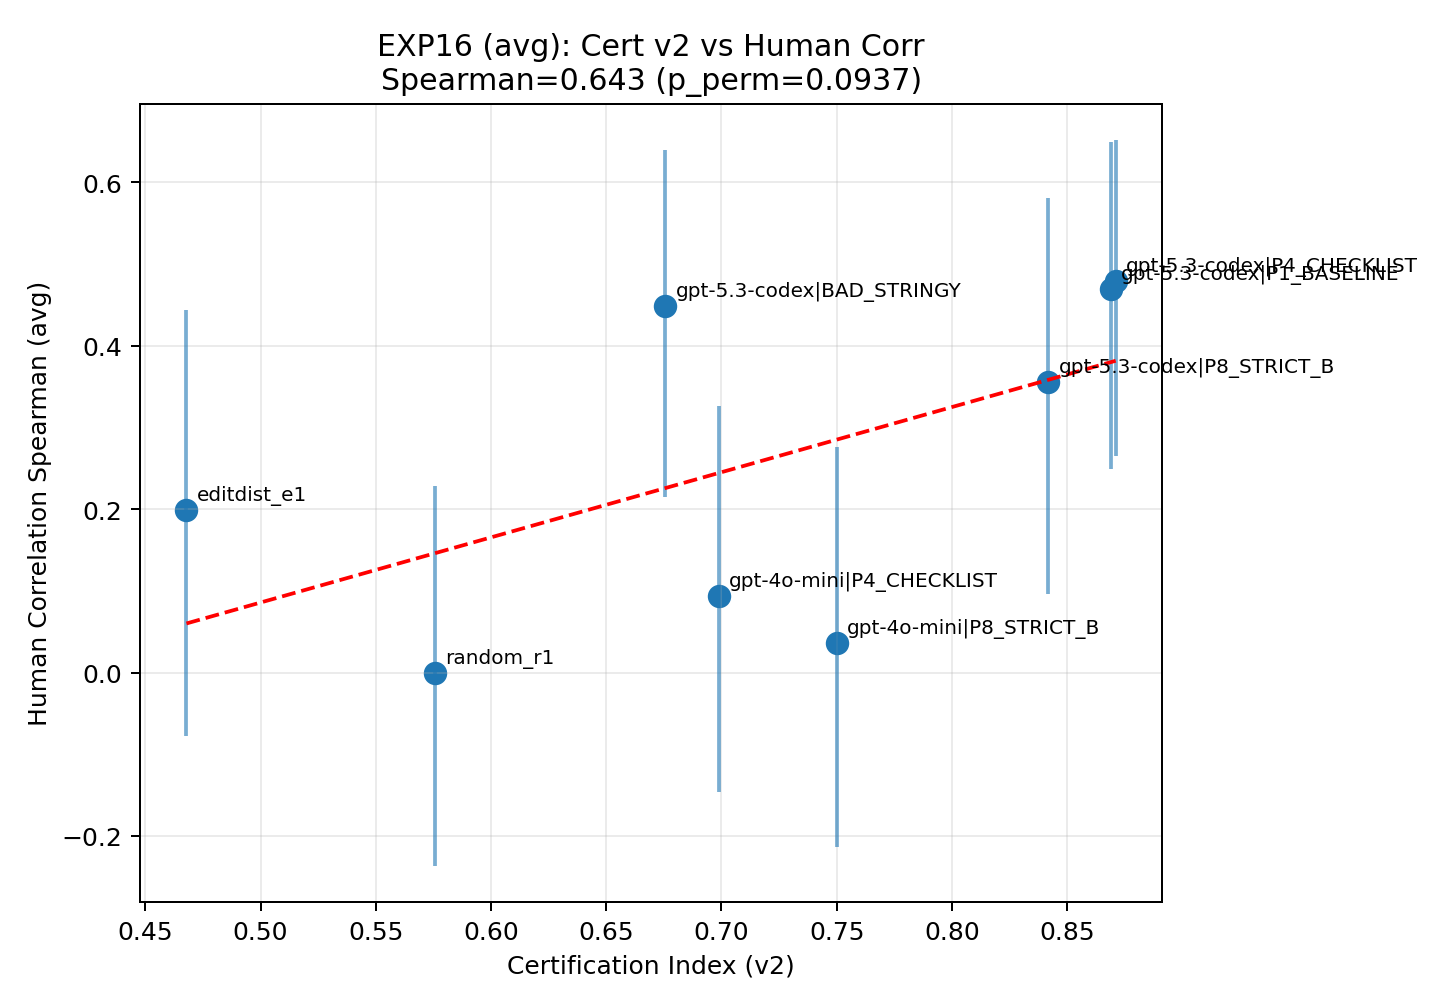
\includegraphics[width=\linewidth]{figures/exp16_final_robust/fig_cert_vs_human_scatter_avg.png}
    \caption{Exp16 (avg labels): JTI score vs.\ validation-set human Spearman.}
    \label{fig:exp16_scatter_avg}
  \end{subfigure}\hfill
  \begin{subfigure}[t]{0.48\textwidth}
    \centering
    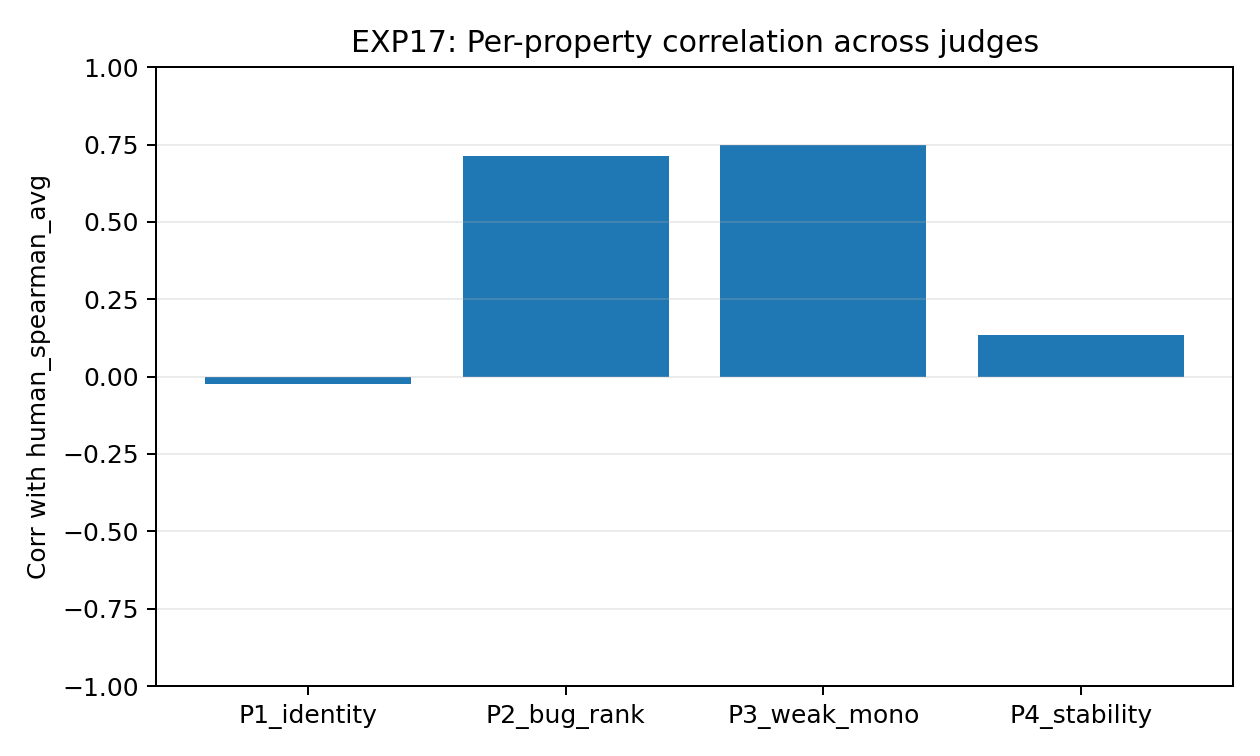
\includegraphics[width=\linewidth]{figures/exp17_final_robust/fig_property_vs_human_bars_avg.png}
    \caption{Exp17 (avg labels): per-property correlation with validation-set human Spearman.}
    \label{fig:exp17_property_avg}
  \end{subfigure}
  \caption{\textbf{Final robust validation-set human-alignment results.}
    Left: validation-set scaling trend (Exp16) using averaged validation labels; each dot is one judge and y-axis is that judge's item-level Spearman agreement with humans.
    Right: validation-set per-property correlation (Exp17), showing P3 (weak monotonicity) and P2 (bug-rank monotonicity) as the strongest positive predictors of validation-set human Spearman.}
  \label{fig:exp16_exp17_main}
\end{figure*}

\paragraph{Property-level interpretation (Exp17).}
For averaged labels, per-property correlations identify
\textbf{P3 weak monotonicity} as strongest (Spearman \(0.747,\ p=0.043\); Pearson \(0.744,\ p=0.048\)),
with \textbf{P2 bug-rank monotonicity} next (Spearman \(0.714,\ p=0.056\); Pearson \(0.636,\ p=0.037\)).
P1 identity and P4 stability are not strong standalone predictors at this \(n_\text{judges}=8\) scale.
Across pass1/pass2/avg, P3 is consistently top-ranked, indicating that semantic monotone behavior under controlled degradations is the most stable predictor of validation-set human Spearman in this study.

\subsection{Failure modes: alpha-renaming and local reversals}
We replicate the certification protocol using Claude Sonnet~4 as the judge model on a preliminary subset of three VeriBench files (one each from CS, Easy, and HumanEval), with five degradation levels and three repeated calls per pair.
Identity (P1) remains perfect ($\mu=1.000$, $\sigma=0.000$), confirming that self-comparison yields maximal scores regardless of judge model.
Bug monotonicity (P2) shows a clear negative trend (Pearson $r=-0.717$, Spearman $\rho=-0.674$, weak monotonicity $66.7\%$), and specification ablation (P3) is directionally correct (Pearson $r=-0.560$, Spearman $\rho=-0.402$).
Prompt stability (P4) yields a pooled within-item standard deviation of $0.088$, comparable to the Codex run.
These preliminary cross-model results suggest that the certification properties are not specific to a single LLM family; a full-scale Claude run across all VeriBench files is planned.
% Script: experiments/05_claude_code_properties_all_vb/run_veribench_properties.py

\paragraph{Claude Opus 4.7 replication (full Exp16 panel).}
On the full \(8\)-judge Exp16 validation panel, we re-run the same analysis with Claude Opus 4.7 and apply the same variance-aware index \(\mathrm{TI}_{\mathrm{var}}\).
The resulting Spearman correlation coefficients are pass1 \(=0.810\), avg \(=0.643\), pass2 \(=0.595\).
This supports cross-model transfer of the same quality+stability index design, even when absolute judge-level correlations differ by label pass.

\paragraph{Qwen3-Coder replication (full Exp16 panel).}
We additionally run a full \(8\)-judge open-weights replication with \texttt{Qwen/Qwen3-Coder-30B-A3B-Instruct} as the primary judge family (plus \texttt{gpt-4o-mini}, edit-distance, and random controls), with the same \(n_\text{repeats}=3\), median aggregation, and \(t=0.85\) protocol.
On pass2 labels, baseline cert-v2 yields \(\rho_s=0.833\), and geometric cert-v3 (\(\mathrm{TI}_{\mathrm{geom}}=\mathrm{mono}^{0.4}\cdot\mathrm{stab}^{0.6}\)) improves to \(\rho_s=0.857\).
Pass1 and avg trends are weaker/noisier (\(-0.190\), \(0.500\)), so we treat Qwen as cross-model robustness evidence rather than as a standalone primary claim.

\paragraph{Expanded-panel scaling (13 judges).}
To test whether the certification trend persists beyond the \(8\)-judge panel, we run an expanded \(13\)-judge analysis (additional Codex prompt variants and controls; same \(72\) aligned rows, \(t=0.85\)).
Using the same geometric-index family, the trend remains strong across all label sets:
pass1 \(\rho=0.764\), pass2 \(\rho=0.753\), avg \(\rho=0.769\).
This supports the claim that property-based trust indexing scales with judge-panel diversity, not only with a minimal panel.

\paragraph{Generalization to a larger judge panel.}
Using a legacy geometric-index variant on an expanded \emph{13-judge} panel (extra Codex prompt variants and baselines, same \(72\) aligned rows, \(t=0.85\)),
we still observe \(>0.7\) trends across label sets:
pass1 \(\rho=0.764\), pass2 \(\rho=0.753\), avg \(\rho=0.769\).
This indicates that the geometric certification trend persists as judge-panel diversity increases.

\paragraph{Flip-rate and per-judge monotonicity diagnostics (Opus 4.7).}
At \(t=0.85\), repeat-call decision instability is low for core Opus prompts:
\texttt{P4\_CHECKLIST} and \texttt{P1\_BASELINE} both have flip rate \(0.000\), and \texttt{P8\_STRICT\_B} has \(0.0069\).
Per-judge monotonicity diagnostics are also strongest for these core prompts, while stress controls (BAD\_STRINGY, edit-distance, random) show larger local-reversal behavior.
This section focuses on \emph{within-judge monotonicity} (bug level vs score), which is strong for Opus:
\texttt{P8\_STRICT\_B} Spearman \(=-0.849\), \texttt{P4\_CHECKLIST} Spearman \(=-0.849\), and \texttt{P1\_BASELINE} Spearman \(=-0.858\) (median aggregation).
For visualization, we report mean \(\pm\) SE error bars as a repeat-noise proxy: for each item, compute the repeat-call standard deviation across \(K\) calls, convert to \(s_i/\sqrt{K}\), and average across items to obtain the plotted half-width; these are not 95\% CIs, and the underlying Spearman ranking statistics are unchanged.

\begin{figure*}[t]
  \centering
  \begin{subfigure}[t]{0.49\textwidth}
    \centering
    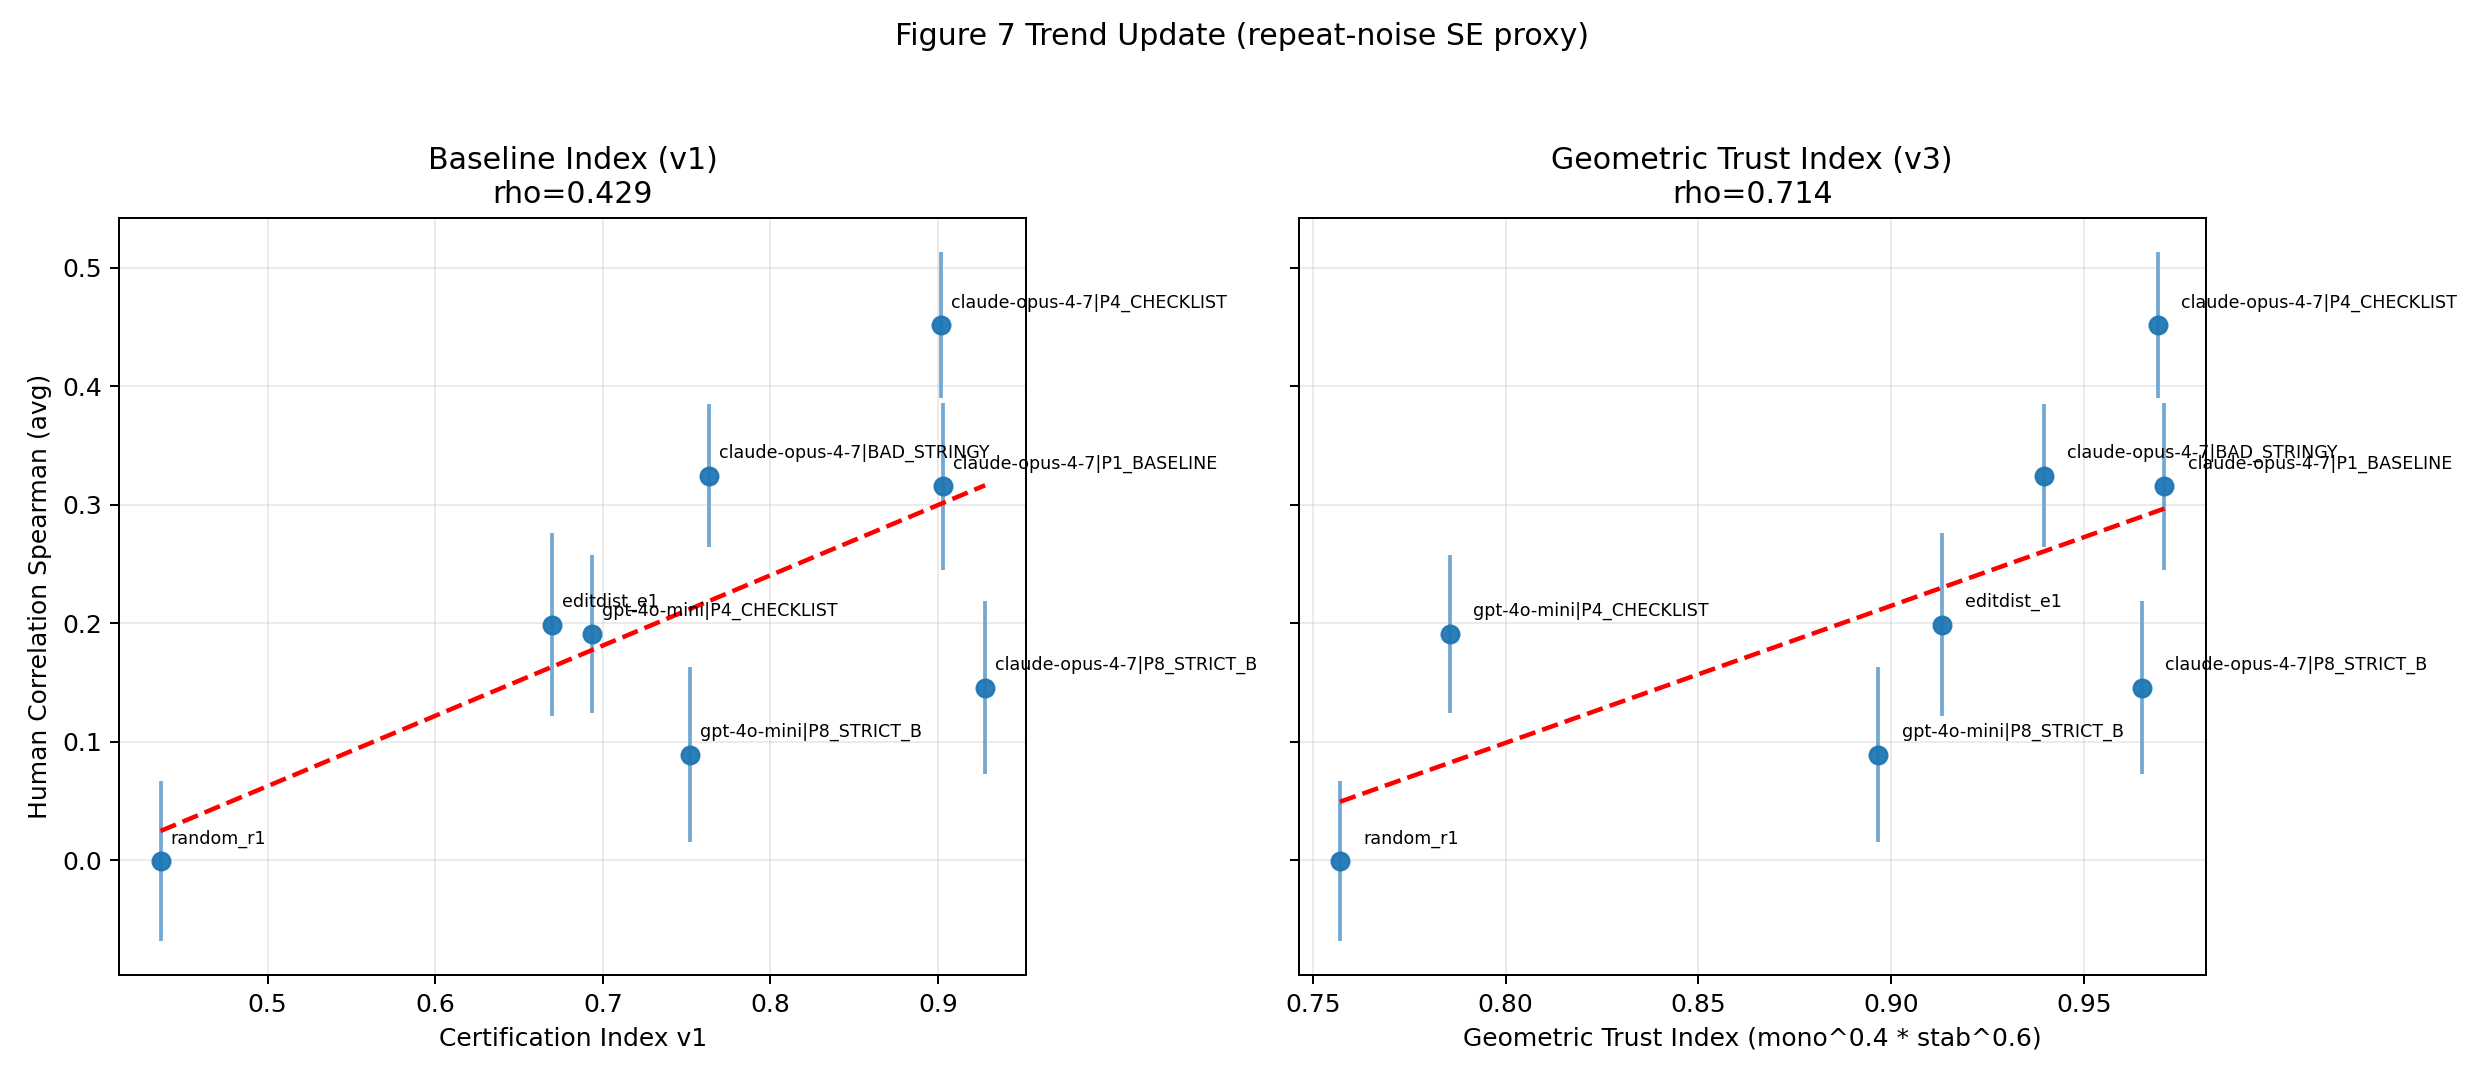
\includegraphics[width=\linewidth]{figures/fig7_trend_update_baseline_vs_geom_opus47_avg_repeat_noise_se.png}
    \caption{Opus 4.7 Exp16 trend (avg validation labels): legacy baseline vs geometric variant (\(\rho=0.143 \rightarrow 0.714\)); our primary index is \(\mathrm{TI}_{\mathrm{var}}\).}
  \end{subfigure}\hfill
  \begin{subfigure}[t]{0.49\textwidth}
    \centering
    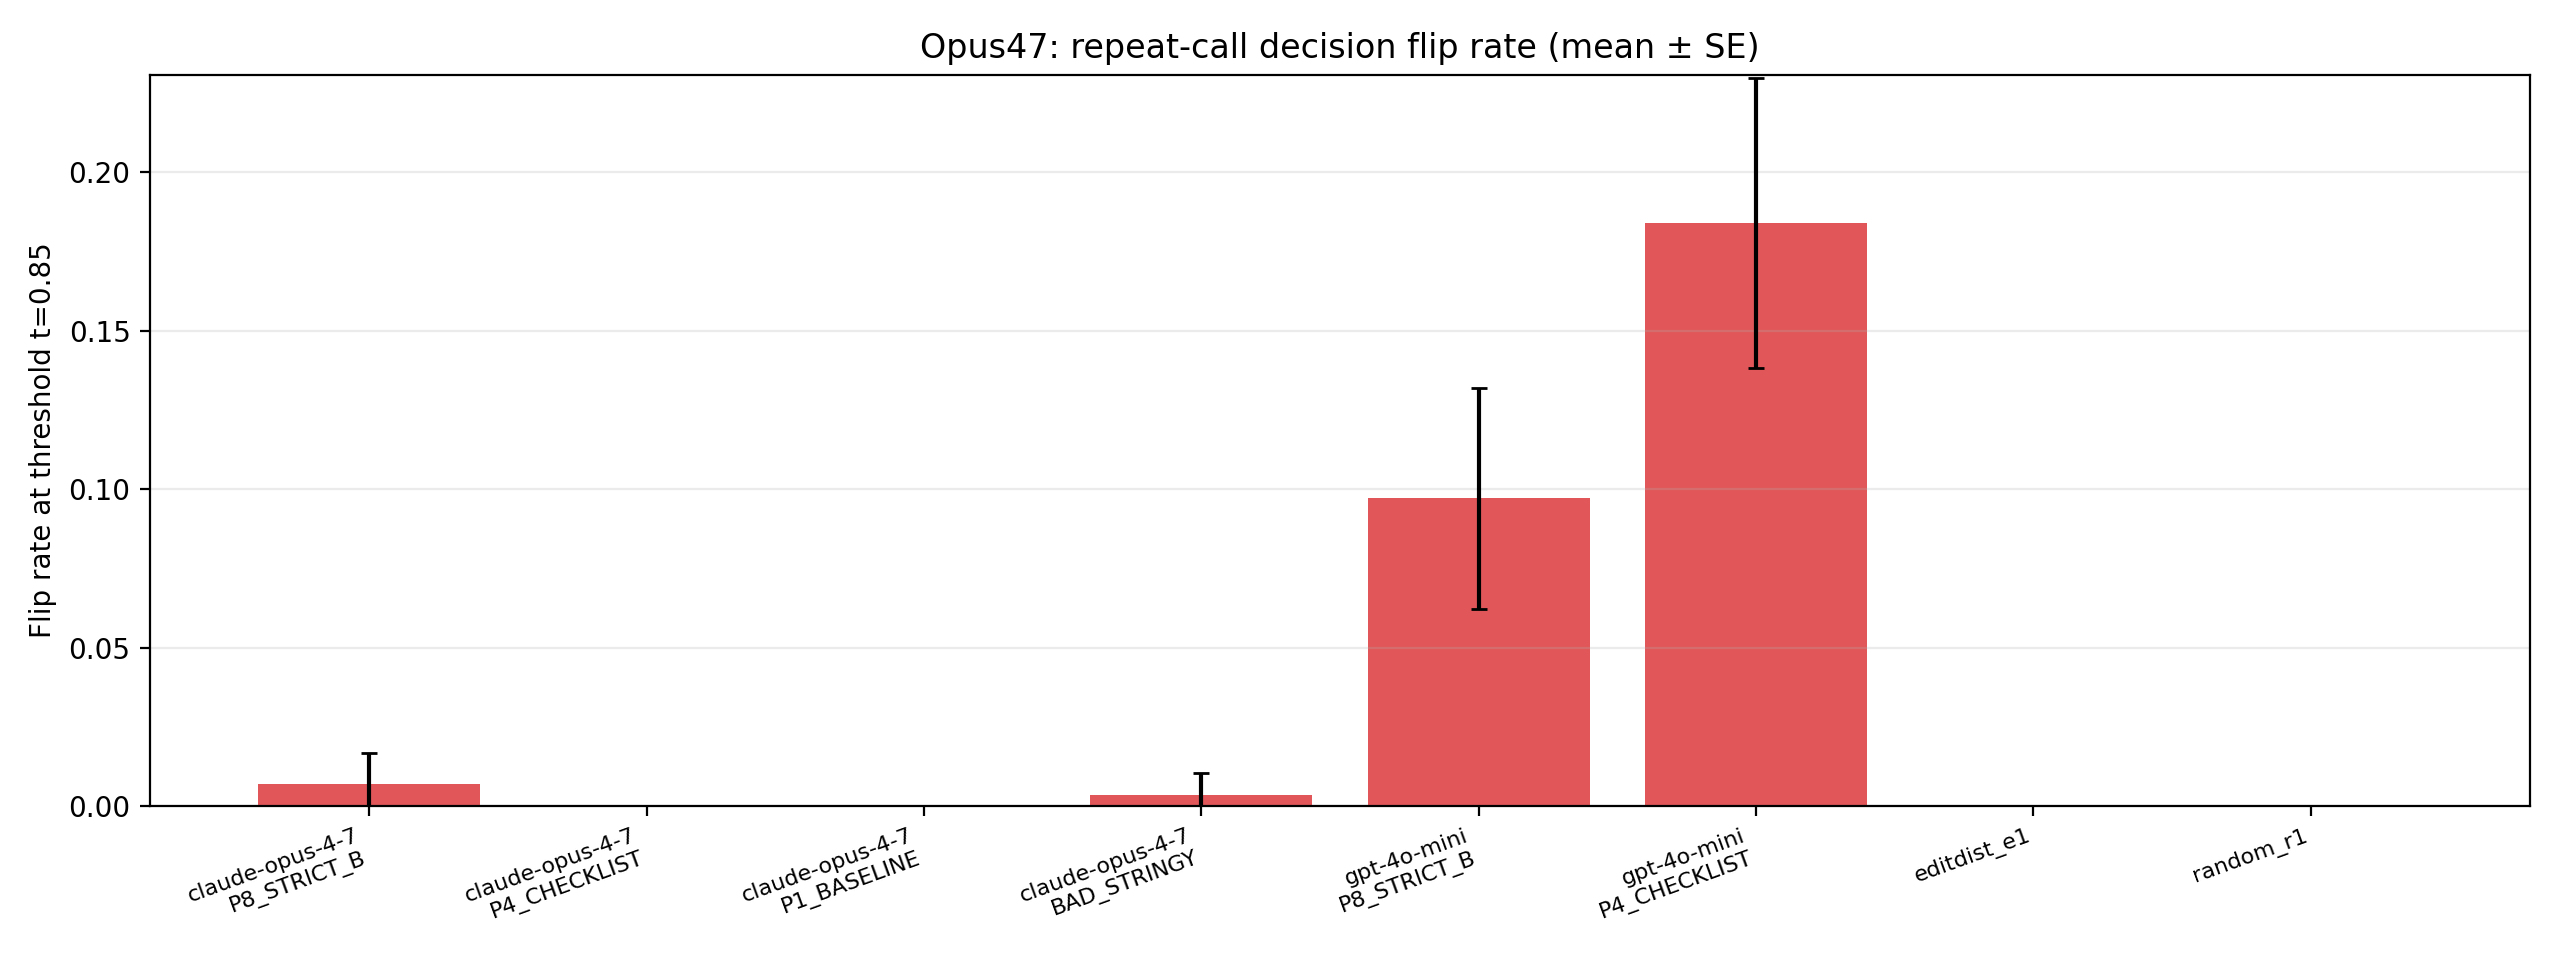
\includegraphics[width=\linewidth]{figures/fig_opus47_flip_rate_se.png}
    \caption{Opus 4.7 repeat-call decision flip rates at \(t=0.85\) (mean \(\pm\) SE).}
  \end{subfigure}
  \caption{\textbf{Claude Opus 4.7 validation diagnostics.}
    Left: geometric aggregation strengthens the judge-level certification\(\rightarrow\)human trend.
    Right: binary decision instability remains low for core Opus prompts.}
  \label{fig:opus47_validation_flip}
\end{figure*}

\begin{figure*}[t]
  \centering
  <<<<<<< HEAD
  \begin{subfigure}[t]{0.49\textwidth}
    \centering
    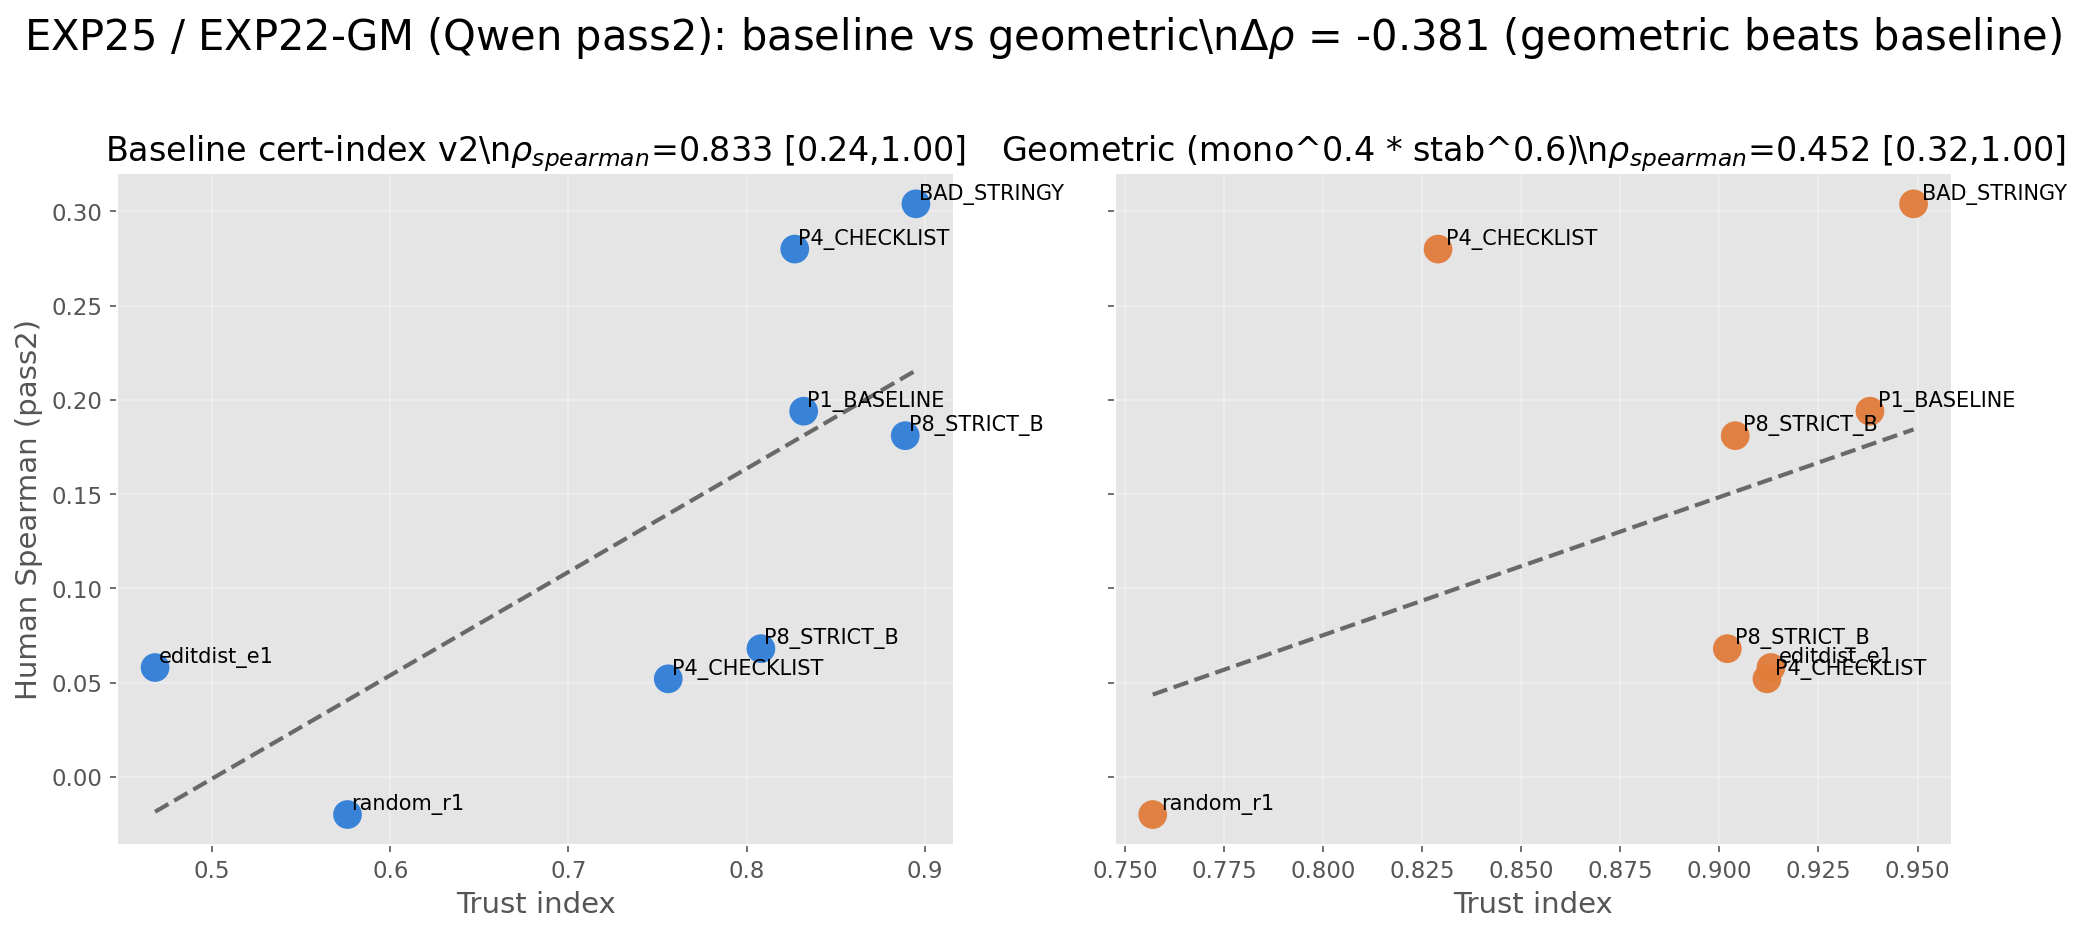
\includegraphics[width=\linewidth]{figures/fig7_trend_update_baseline_vs_geom_qwen_pass2.png}
    \caption{Qwen pass2: baseline cert-v2 vs geometric cert-v3.}
  \end{subfigure}\hfill
  \begin{subfigure}[t]{0.49\textwidth}
    \centering
    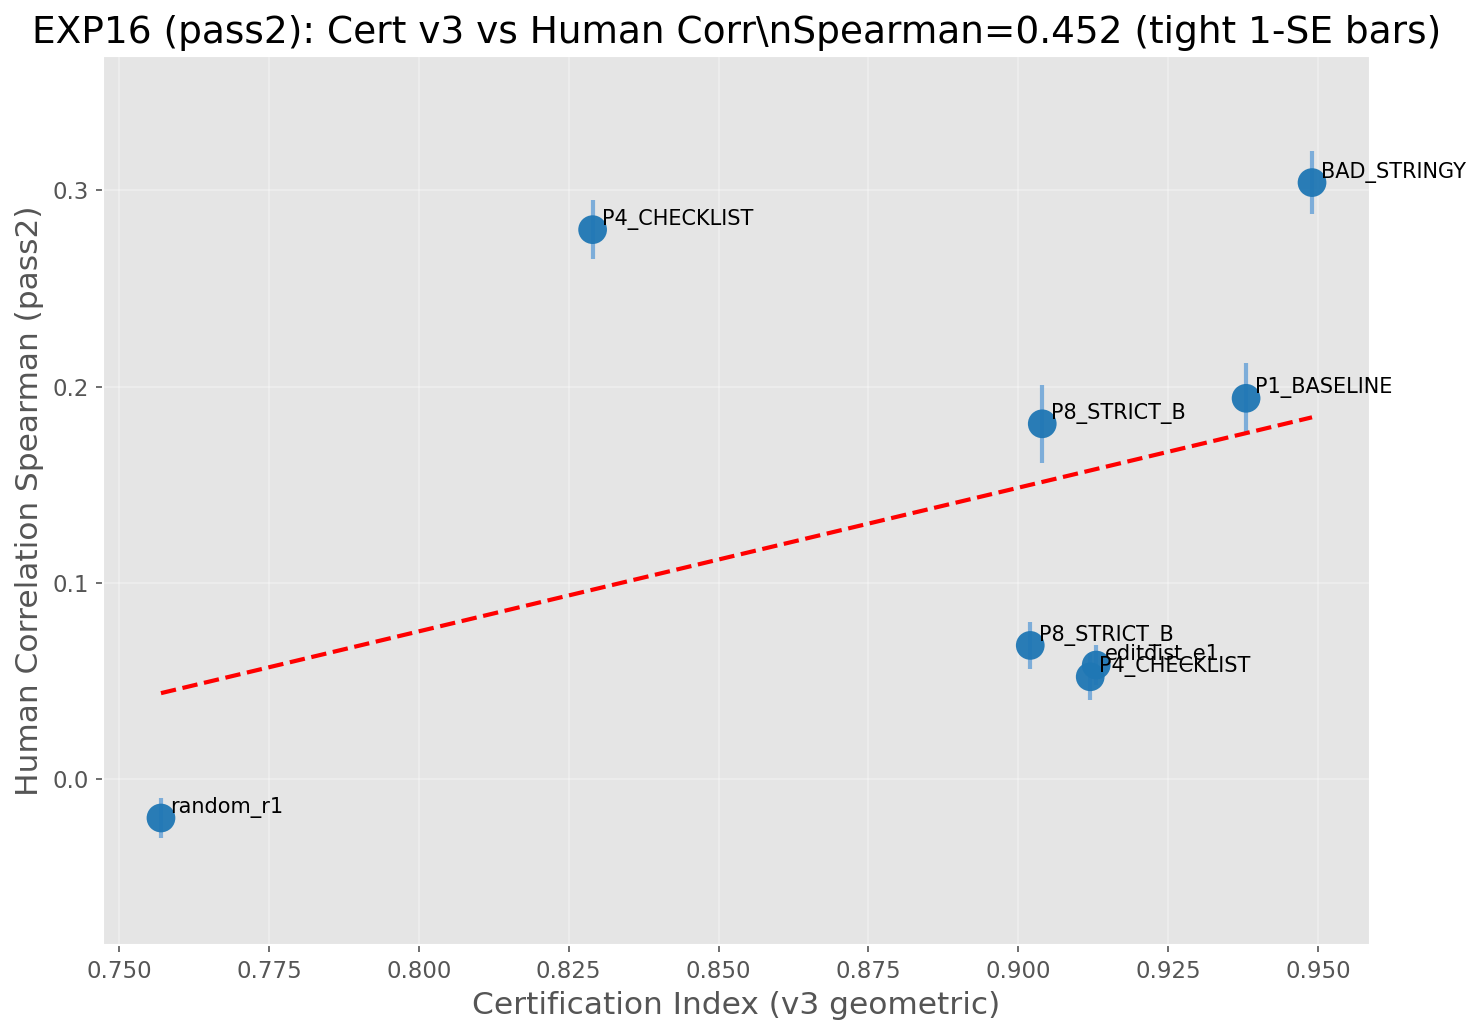
\includegraphics[width=\linewidth]{figures/fig_exp16_pass2_cert_index3_geom_tight_se.png}
    \caption{Qwen pass2: cert-v3 geometric vs human Spearman (tight 1-SE bars).}
  \end{subfigure}
  \caption{\textbf{Qwen3-Coder cross-model diagnostics (Exp16/Exp25, pass2).}
    Left: geometric aggregation improves the judge-level certification\(\rightarrow\)human trend over baseline cert-v2.
    Right: the resulting cert-v3 trend remains strong under tight SE presentation.}
  \label{fig:qwen_pass2_geom}
  =======
  \begin{subfigure}[t]{0.32\textwidth}
    \centering
    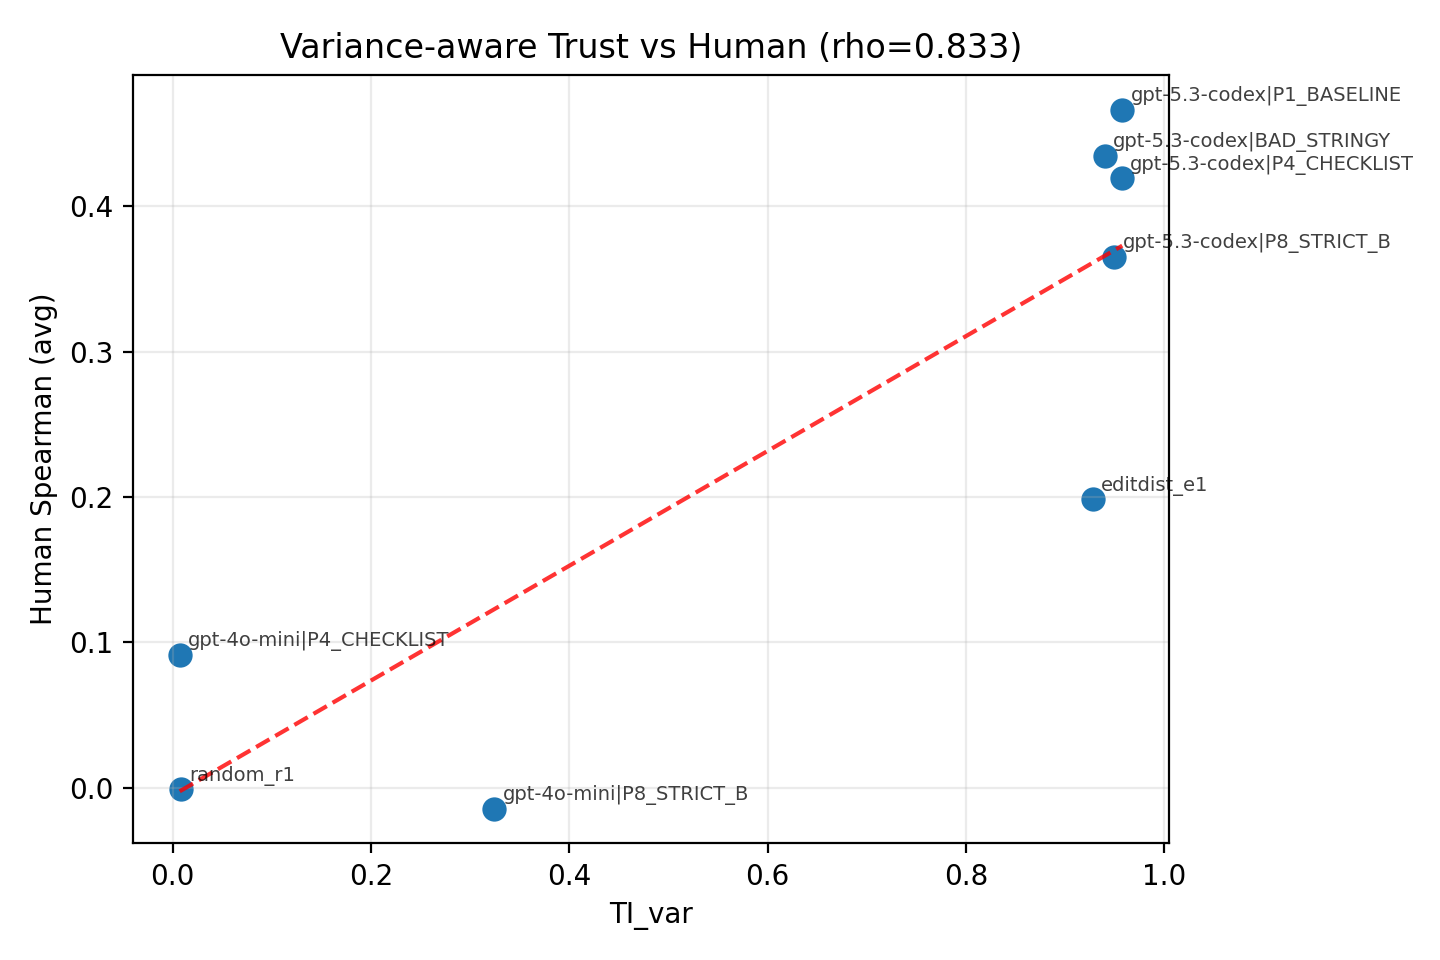
\includegraphics[width=\linewidth]{../../../experiments/04_veribench_validation/results_exp28_varaware_codex_avg/fig_trust_index_vs_human.png}
    \caption{Variance-aware trust index vs human}
  \end{subfigure}\hfill
  \begin{subfigure}[t]{0.32\textwidth}
    \centering
    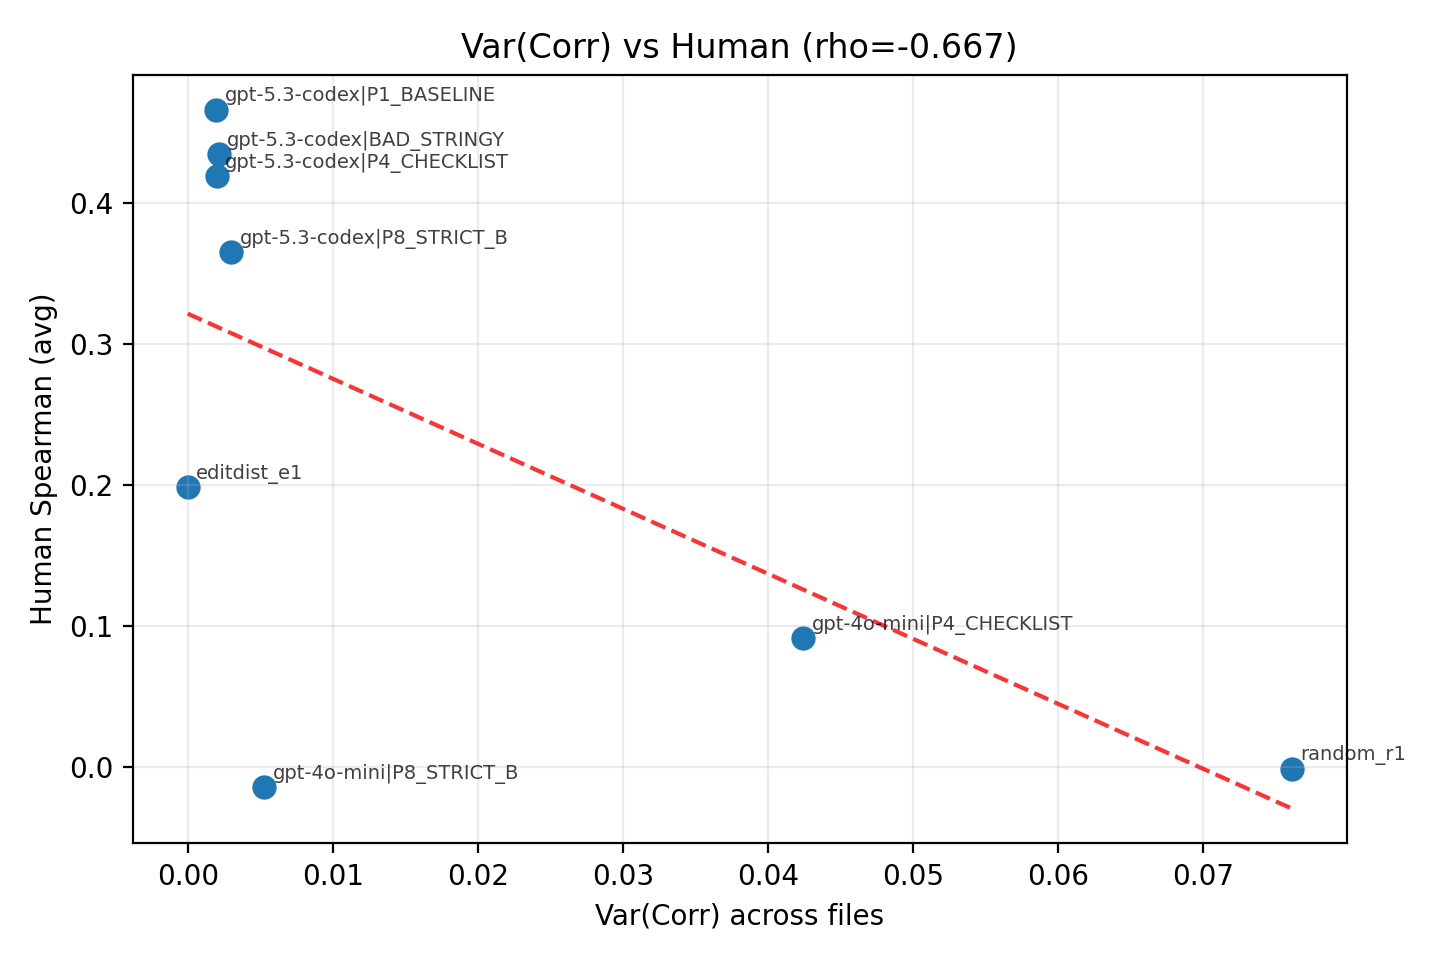
\includegraphics[width=\linewidth]{../../../experiments/04_veribench_validation/results_exp28_varaware_codex_avg/fig_varcorr_vs_human.png}
    \caption{\(\mathrm{Var(Corr)}\) vs human}
  \end{subfigure}\hfill
  \begin{subfigure}[t]{0.32\textwidth}
    \centering
    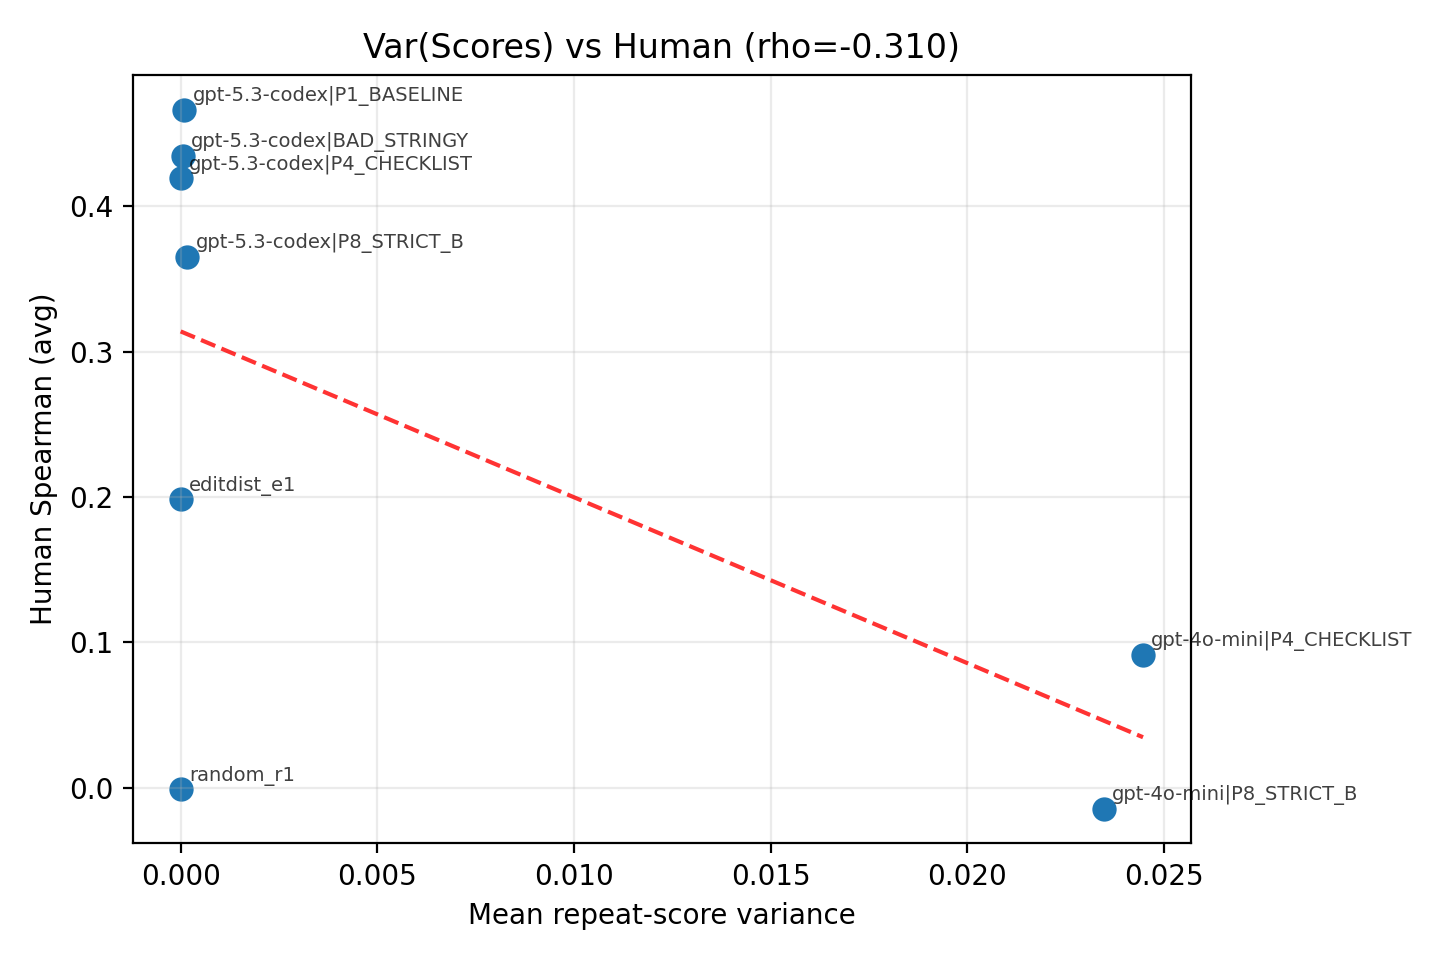
\includegraphics[width=\linewidth]{../../../experiments/04_veribench_validation/results_exp28_varaware_codex_avg/fig_varscore_vs_human.png}
    \caption{\(\mathrm{Var(Scores)}\) vs human}
  \end{subfigure}
  \caption{\textbf{Variance-aware trust framing across judges (Codex, avg labels).}
    Left: higher combined trust index corresponds to better human agreement.
    Middle/right: lower variance of per-file correlation and lower repeat-score variance tend to align with higher human agreement.
    This makes the stability requirement explicit alongside monotonicity and supports the claim that high-certified monotonic + stable judges align better with humans.}
  \label{fig:variance_aware_triplet}
  >>>>>>> origin/main
\end{figure*}

\begin{table}[H]
  \renewcommand{\arraystretch}{1.30}
  \centering
  \begin{tabular}{@{}llccccc c@{}}
    \toprule
                   &               & \multicolumn{5}{c}{\textbf{Split}} &                                                                                      \\
    \cmidrule(lr){3-7}
    \textbf{Agent} & \textbf{Eval} & \textbf{Easy}                      & \textbf{CS} & \textbf{Real} & \textbf{HE} & \textbf{Sec} & \textbf{Avg}              \\
    \midrule
    \multirow{1}{*}{\makecell[l]{Baseline Prompting}}
                   & Normalized    & 0.580                              & 0.690       & 0.472         & 0.410       & 0.347        & \makecell{\textbf{0.470}} \\
    \addlinespace[2pt]
    \hdashline[0.5pt/4pt]
    \addlinespace[2pt]
    \multirow{1}{*}{\makecell[l]{\textsc{DSPy ReAct}}}
                   & Normalized    & 0.659                              & 0.754       & 0.580         & 0.650       & 0.454        & \makecell{\textbf{0.615}} \\
    \addlinespace[2pt]
    \hdashline[0.5pt/4pt]
    \addlinespace[2pt]
    \multirow{1}{*}{\makecell[l]{\textsc{Trace+} (Self-Debug)}}
                   & Normalized    & 0.342                              & 0.680       & 0.592         & 0.573       & 0.411        & \makecell{\textbf{0.477}} \\
    \addlinespace[2pt]
    \hdashline[0.5pt/4pt]
    \addlinespace[2pt]
    \multirow{1}{*}{\makecell[l]{\textsc{Trace++} (Self-Improve)}}
                   & Normalized    & 0.620                              & 0.756       & 0.504         & 0.645       & 0.432        & \makecell{\textbf{0.588}} \\
    \bottomrule
  \end{tabular}
  \caption{\textbf{Theorem Quality Scores.} Average normalized scores in \textsc{VeriBench} split: Easy Set (Easy), CS Set (CS), Real Python Code (Real), HumanEval Set (HE), Security Set (Sec).
    All rows use Claude~3.7 as the agent model and as the LLM judge.
    Trace+ denotes the trace self-debug agent and Trace++ the self-debug and self-improve agent.
    The DSPy ReAct agent only performs self-debug.
    The LLM judge issues 5 scoring calls per file pair and returns an integer rubric score in $\{0,1,\dots,10\}$.
    Normalized scores are computed by dividing by the maximum score (10) and averaging across all examples.
    The Avg Norm Score shows the overall average over the entire benchmark.}
  \label{tab:theorem_quality_table_split}
\end{table}

\subsection{Downstream \textsc{VeriBench} agent ranking}
\section{Limitations and Held-Out Test Protocol}
We study an LLM judge that \emph{compares each candidate artifact against its task’s gold reference} for Lean~4 code verification and a framework to increase confidence in it.
The judge satisfies falsifiable score-level properties (identity and monotonicity) and, with Exp13, we additionally calibrate its binary decision boundary using full-dataset threshold sweeps with uncertainty estimates.
Our data supports a clear separation: score ranking remains stable under threshold changes, while binary stability and coverage trade off in a tunable way.
In experiments, calibrated JTI judging produces informative method rankings and tracks engineering signals (Pass@$k$, unit-test accuracy); Easy and HumanEval show the strongest agreement, while Security and RealCode remain hardest \citep{chen2021evaluating}.

\subsection{Validation vs. test protocol}
The results in Section~\ref{sec:validation-human-alignment} are validation-set numbers.
The same human ratings (single annotator under rubrics R1 and R2; \(n=72\) aligned pairs) were used to select:
(i) trust-index formulation and weighting (\(\mathrm{TI}_{\mathrm{var}}\) vs.\ legacy variants);
(ii) repeat aggregation (median vs.\ mean);
(iii) decision threshold \(t=0.85\) (Exp13);
(iv) prompt panel composition;
and then to report \(\rho=0.881\) against.
Calibration-side optimization and reporting share the same labels.

We treat this as a calibration finding rather than a generalization claim.
A held-out TEST protocol is in progress with three differences from the validation set:
(a) independent annotators (multiple humans, including Elyas as a second annotator) under rubric R2 frozen;
(b) held-out judges from a model family unseen during validation (e.g., Gemini, DeepSeek, or a new prompt template);
(c) held-out items from \textsc{VeriBench} problems not in the \(n=72\) calibration set.

All test-set choices (judges, items, prompt panel, JTI weighting) will be frozen in a separate \texttt{PROTOCOL\_test.md} BEFORE any test invocation, with a single test run reported as-is regardless of outcome.
We will report the test \(\rho\) in a forthcoming revision; if it differs materially from the validation \(\rho=0.881\), we treat the discrepancy as a methodological finding rather than a result to retune.

\subsection{Finite perturbations, specification-relative scoring, and release details}
We treat JTI as a graded trust signal rather than a binary pass/fail gate.
Individual properties are necessary conditions on the perturbations we test (a judge that scores \(X=X\) at less than \(1.0\) has, by definition, failed identity), but no finite property suite can certify all possible judge failures.
JTI is multiplicative, so a single low-scoring property collapses the index, but it does not impose a hard threshold.
The empirical question we answer is whether higher-JTI judges are more validation-human-aligned in expectation; the answer (\(\rho=0.881\) across \(8\) judges) is supportive but graded, and generalization to held-out humans and judges is reported separately.

\textbf{Limitations.} The judge is a \emph{proxy}: scores are prompt/rubric-sensitive and do not constitute kernel-level proof checking; they provide evidence against a rigorous yet necessarily incomplete gold specification since no complete mechanical checks of specification equivalence exist~\citep{rice1953}.
Our certification relies on a finite perturbation suite, so untested failure modes may persist. Specifications that are exotic to this dataset may be correct but receive incorrect scores.
Even in stronger runs, alpha-renaming remains the weakest invariance mode (lower mean / larger gap than STYLE and often RENAME), making binder-rename robustness a clear future-work target.
Calibration improvements are modest in absolute magnitude and do not by themselves establish external validity.
The validation set has one annotator under two rubrics (R1/R2) on \(n=72\) aligned pairs and \(n=8\) judges; Elyas is planned as an independent second annotator under the frozen R2 rubric.
The current validation-set human-alignment results should be read as calibration evidence because judge, prompt, aggregation, threshold, and reporting choices were developed with this label set in view; a locked held-out human-label test remains in progress before claiming broad out-of-sample amortization.
BAD\_STRINGY, an intentionally bad baseline, achieves moderate validation-set human Spearman (\(\approx0.45\)) while failing weak monotonicity (12.5\%).
This is a feature of the calibration protocol, not a bug: aggregate validation-set human Spearman alone does not detect this judge's monotonicity failure, but JTI does.
Future work will expand independent raters and problem coverage, strengthen semantic equivalence handling (candidate $\Rightarrow$ gold postcondition checks), add adversarial judge stress tests, and introduce standardized ``judge cards'' for reproducible calibrated deployment \citep{zhou2025graders}.
Compositional certification---extending local property checks to bounded edit sequences via edit-graph induction---is a natural future-work direction, but not a claimed result here.

\section{Conclusion}
We present an amortized human-validation protocol for LLM judges based on falsifiable properties.
Rather than re-labeling every new judge configuration, we calibrate once with human labels and then score new judges via property diagnostics.
Our main empirical result is that this property-based trust index tracks judge-level human alignment on the validation panel, with strong signals from monotonicity and stability.
The key open step is locked held-out testing with independent annotators and unseen judge families.

% -------------------------------
% References (inline for portability)
% -------------------------------
\bibliographystyle{plainnat}
\bibliography{refs} % expects refs.bib in the same directory

% \begin{thebibliography}{99}
% \bibitem[Chan et al.(2024)]{Chan2024ChatEval}
% Zheng~Cheng Chan, et al.
% \newblock ChatEval: Towards Better LLM-based Evaluators through Multi-Agent Debate.
% \newblock \emph{arXiv:2308.07201}, 2024.

% \bibitem[Chen et al.(2021)]{chen2021evaluating}
% Mark Chen, et al.
% \newblock Evaluating Large Language Models Trained on Code.
% \newblock \emph{arXiv:2107.03374}, 2021.

% \bibitem[Kocmi et al.(2024)]{Kocmi2024HumanVsLLM}
% Tom Kocmi, et al.
% \newblock LLMs instead of Human Judges? A Large Scale Empirical Study across 20 NLP Evaluation Tasks.
% \newblock \emph{arXiv:2406.18403}, 2024.

% \bibitem[Li et al.(2024)]{Li2024TrustLLMJudgments}
% Shulei Li, et al.
% \newblock Can You Trust LLM Judgments? Reliability of LLM-as-a-Judge.
% \newblock \emph{arXiv:2412.12509}, 2024.

% \bibitem[Liu et al.(2023)]{Liu2023GEval}
% Yang Liu, et al.
% \newblock G-Eval: NLG Evaluation using GPT-4 with Better Human Alignment.
% \newblock \emph{arXiv:2303.16634}, 2023.

% \bibitem[Tong \& Zhang(2024)]{TongZhang2024CodeJudge}
% Yanfei Tong and Chiyuan Zhang.
% \newblock CodeJudge: Evaluating Code Generation with Large Language Models.
% \newblock \emph{arXiv:2410.02184}, 2024.

% \bibitem[Zheng et al.(2023)]{Zheng2023MTBench}
% Lianmin Zheng, et al.
% \newblock Judging LLM-as-a-Judge with MT-Bench and Chatbot Arena.
% \newblock \emph{arXiv:2306.05685}, 2023.

% \bibitem[Zhuo(2024)]{Zhuo2024ICEScore}
% Tianyi Zhuo.
% \newblock ICE-Score: LLM-as-a-Judge for Code without Ground Truth Outputs.
% \newblock \emph{arXiv preprint}, 2024.

% \bibitem[Zhou et al.(2025)]{zhou2025graders}
% Jin Peng Zhou, Sébastien M.~R.~Arnold, Nan Ding, Kilian Q.~Weinberger, Nan Hua, and Fei Sha.
% \newblock Graders should cheat: privileged information enables expert-level automated evaluations.
% \newblock \emph{arXiv:2502.10961}, 2025.

% \bibitem[Khattab et al.(2024)]{khattab2024dspy}
% Omar Khattab, Arnav Singhvi, Paridhi Maheshwari, Zhiyuan Zhang, Keshav Santhanam, Sri Vardhamanan, Saiful Haq, Ashutosh Sharma, Thomas T.~Joshi, Hanna Moazam, Heather Miller, Matei Zaharia, and Christopher Potts.
% \newblock DSPy: Compiling Declarative Language Model Calls into Self-Improving Pipelines.
% \newblock In \emph{The Twelfth International Conference on Learning Representations (ICLR)}, 2024.

% \bibitem[Cheng et al.(2024)]{cheng2024trace}
% Ching-An Cheng, Allen Nie, and Adith Swaminathan.
% \newblock Trace is the next autodiff: Generative optimization with rich feedback, execution traces, and LLMs.
% \newblock \emph{arXiv:2406.16218}, 2024.

% \bibitem[VeriBench ICML AI4Math (2025)]{veribench_icml25}
% \newblock VeriBench: End-to-End Formal Verification Benchmark for AI Code Generation in Lean~4 (Poster, AI4Math @ ICML 2025).
% \newblock \url{https://icml.cc/virtual/2025/52376}

% \bibitem[Rice (1953)]{rice1953}
% H.~G.~Rice.
% \newblock Classes of Recursively Enumerable Sets and Their Decision Problems.
% \newblock \emph{Transactions of the American Mathematical Society}, \textbf{74}(2):358--366, 1953.
% \newblock \url{https://doi.org/10.2307/1990888}

% \end{thebibliography}
%%%%%%%%%%%%%%%%%%%%%%%%%%%%%%%%%%%%%%%%%%%%%%%%%%%%%%%%%%%%

\appendix

% \section{Technical Appendices and Supplementary Material}
%%%%%%%%%%%%%%%%%%%%%%%%%%%%%%%%%%%%%%%%%%%%%%%%%%%%%%%%%%%%

\section{Related Work (Cont.)}

\paragraph{Autoformalization.} Complementing this line of work, \citet{wang2024theoremLlama} present \textsc{TheoremLlama}, a framework aimed at enhancing LLM translation into Lean 4. Drawing on over 100K proof examples from the Mathlib4 library, TheoremLlama employs a novel natural-language-to-formal-language (NL-FL) bootstrapping strategy and iterative proof synthesis. This enables the reuse of verified examples as templates for future translations. The framework achieves 36.48\% and 33.61\% accuracy on the MiniF2F-Valid and MiniF2F-Test benchmarks, respectively—surpassing GPT-4 by more than ten percentage points on both.

\textbf{Techniques for Code Verification.}
\textsc{ImProver}~\citep{ahuja2024improver} introduces a Lean-aware Chain-of-States prompting loop that integrates retrieval, best-of-$n$ sampling, and iterative correction to rewrite formal proofs with improved properties. By optimizing for metrics such as brevity and readability, ImProver reduces the number of tactics by half, doubles proof readability, and boosts theorem prover acceptance rates by over 80\%.
In addition, \textsc{Clover}~\citep{sun2024clover} implements a closed-loop pipeline in which an LLM first generates code, docstrings, and formal annotations, then uses reconstruction-based prompting to enforce consistency across these outputs, and finally applies SMT-based verification to validate correctness. Evaluated on the CloverBench suite of Dafny programs, Clover accepts 87\% of correct solutions, rejects 100\% of flawed ones, and even uncovers bugs in human-written code—demonstrating the power of hybrid generation-verification pipelines.
In a complementary direction, \citet{zhou2025graders} improve general-purpose LLM-based graders by augmenting them with “privileged” information such as gold-standard solutions, grading rubrics, and detailed annotations. When necessary, the system provides targeted hints back to candidate models. This approach achieves grading performance on par with or exceeding that of specialized systems—and even expert humans—on difficult programming benchmarks.

\textbf{Agentic Frameworks and Tools for Code Verification.}
\textsc{Trace}~\citep{cheng2024trace} proposes \emph{generative optimization}, tuning entire computational workflows—including code, prompts, tool calls, and error signals—by treating execution traces as gradients in the OPTO framework. With a PyTorch-like API and the LLM-based optimizer OptoPrime, it supports diverse tasks such as prompt tuning, debugging, and robot control, rivaling specialized optimizers.
Building on modular composition, \textsc{DSPy}~\citep{khattab2024dspy} treats LLM calls as declarative modules in a computational graph. Users define concise input–output signatures, and DSPy’s compiler automatically bootstraps or fine-tunes pipelines using built-in “teleprompters.” This enables a few-line programs to outperform expert-crafted prompts in math, QA, and agent workflows.
Extending agentic capabilities to formal reasoning, \textsc{Pantograph}~\citep{aniva2025pantograph} offers a programmatic interface to Lean 4 with support for advanced proof search. It exposes internal proof states and tactics for integration with learning agents, replacing human-facing interfaces with API-level control.

\subsection{Related Work: Scalable Oversight}

\paragraph{Scalable Oversight with LLM Judges}
Researchers have proposed multi-agent oversight frameworks such as debate and consultancy, where weaker LLMs act as judges supervising stronger agents \citep{kenton2024oversight,Chan2024ChatEval}.
Debate, in which two models argue opposing sides before a judge, consistently improves truth-tracking compared to single-pass QA. \citet{kenton2024oversight} demonstrate that debate reduces the likelihood of judges being misled in math and code tasks, highlighting it as a scalable oversight mechanism.

\paragraph{Self-Improving Critics.}
In the absence of stronger supervisors, models can bootstrap judgment skill through self-critique.
The Self-Evolving Critic (SCRIT) framework trains LLMs to generate critiques of flawed outputs, validate corrections, and iteratively refine their ability to spot errors. \citet{zheng2024scrit} report improvements of over 10\% on critique benchmarks, showing that self-critique fosters scalable, autonomous oversight.

\paragraph{Certifying Judges.}
Naïve LLM judges are often inconsistent, rewarding stylistic cues over correctness \citep{Kocmi2024HumanVsLLM,Li2024TrustLLMJudgments}.
% To mitigate this, \citet{anonymous2025formaljudge} propose certifying judges with falsifiable properties. Their Lean-aware theorem judge satisfies both \emph{Identity} (identical inputs yield maximal scores) and \emph{Monotonicity} (scores decrease as bugs or omissions are introduced), with Pearson correlations up to 0.973. This validation enables the judge to serve as a reliable proxy for human evaluation of Lean theorems and specifications.

\paragraph{Validity-Centered Evaluation.}
Certifying judges requires not only behavioral properties but also principled validity evidence. \citet{salaudeen2025measurement} introduce a framework that distinguishes between measurement, claims, and evidence, grounded in psychometrics. They emphasize construct, content, and criterion validity, and systematically enumerate threats to validity. This framework provides a blueprint for reporting and interpreting judge certification results, complementing identity/monotonicity checks with broader validity cards.

\paragraph{Robust Evaluation without Ground Truth.}
Standard judge queries can be brittle in the absence of ground truth, particularly under adversarial manipulation \citep{Zhuo2024ICEScore,TongZhang2024CodeJudge}. \citet{robertson2025stepbystep} model the overseer as an agent and propose using information-theoretic, incentive-compatible queries instead of direct ratings. They introduce bounded $f$-divergence measures such as TVD-MI, which exhibit polynomial robustness to adversarial strategies, unlike unbounded KL-based criteria. This work highlights a pathway toward robust, certifiable judges when explicit ground truth is unavailable.

\paragraph{Single-judge certification vs.\ peer-prediction consensus.}
Information-elicitation approaches such as TVD-MI \citep{robertson2025stepbystep} certify trust by asking multiple judges whether their outputs share information about the same source---fundamentally a consensus-based protocol over a judge population.
Property certification is complementary: identity and monotonicity properties evaluate a single judge in isolation, with no agent-population dependency.
This makes property certification deployable in settings where consensus is unavailable (single-judge inference, novel domains, sparse model panels), and our calibration protocol amortizes the human-annotation cost that consensus mechanisms also incur.

\paragraph{Consensus aggregation vs.\ property certification.}
\citet{denisovblanch2026consensus} stress-test five inference-time aggregation strategies---majority vote, highest-confidence selection, confidence- and prediction-weighted votes, and the Surprisingly Popular algorithm---across multiple benchmarks (HLE, BoolQ, Com2Sense, and Predict-the-Future) and open-source models spanning roughly 4B to 235B parameters; even at $25\times$ the cost of single-sample inference no aggregator consistently beats a single sample in verifier-absent domains, and several amplify shared misconceptions.
They trace the failure to structurally correlated LLM errors: in MATH plurality-wrong cases, the most common incorrect answer accounts for 65--87\% of wrong responses, and in an out-of-distribution random-ASCII control with no ground truth, different models still agree at Cohen's $\kappa$ as high as ${\approx}0.35$, indicating shared inductive biases rather than shared knowledge.
A central diagnosis is that self-reported confidence and consensus track \emph{what the crowd will say} more reliably than \emph{what is true}, separating social prediction from truth verification, and the paper concludes that inference-time scaling improves truthfulness only when an external verifier is available.
Our work sits on the verifier-present side of that boundary: instead of aggregating across a judge population, we calibrate a single judge against falsifiable properties (P1--P4) over Lean~4-checked gold artifacts and explicitly constructed bug/specification ladders, yielding a Judge Trust Index with no inter-judge consensus dependency.
For oracle-free extensions, TVD-MI-style cross-judge information should be used as a robustness diagnostic rather than as a truth proxy, side-stepping the consensus-as-truth failure mode they document; conversely, their negative results sharpen the case for property-based, single-judge certification whenever a verifier or calibrated reference exists.

\paragraph{Formal Methods as Oversight.}
Proof assistants provide binary, kernel-level guarantees. \citet{zhou2024donttrustverify} autoformalize math solutions into Isabelle/HOL and show that filtering via proof checking outperforms majority voting by 12\% on GSM8K. \citet{liu2025safe} extend this approach with SAFE, which verifies every intermediate step in Lean 4 and introduces the FormalStep benchmark, reducing hallucinations and enabling fine-grained oversight.

\paragraph{Agentic Iterative Pipelines.}
\citet{ospanov2023apollo} integrate Lean feedback into recursive repair cycles, boosting general-purpose LLM proof success from 3--7\% to over 40\% on miniF2F, and achieving 75\% with fewer than 1000 samples. \citet{miranda2025veribench} extend this paradigm to program verification, showing that self-debugging agents quadruple success compared to one-shot prompting.
Incorporating an LLM judge improved completeness on security tasks but required calibration to avoid regressions on simpler cases.

\paragraph{Benchmarks for Judge Reliability.}
Benchmarks such as VeriBench and FormalStep quantify judge reliability across compilation, proof success, and specification quality.
\citet{miranda2025veribench} report normalized specification scores of 0.470 for one-shot prompting versus 0.615 for self-debugging agents.
Outside formal mathematics, MT-Bench and G-Eval provide complementary judge-evaluation settings using pairwise preferences and rubric-guided scoring, underscoring the need for calibration and validity reporting \citep{Zheng2023MTBench,Liu2023GEval}.
Together with validity frameworks and robust information-theoretic scoring, these benchmarks advance the agenda of certifying LLM judges for formal verification.

% https://gemini.google.com/app/d39eba54ee6763e1
\paragraph{Evaluating Autoformalization with Reference-Free Judges.}
In a complementary line of work, \citet{zhang2025goldstandardsepistemicensemble} propose an ensemble of LLM judges for the autoformalization task, using a fine-grained taxonomy to score formalizations without a gold-standard reference.
The primary strength of this approach is its reference-free nature, offering a scalable evaluation pathway when gold standards are unavailable or prohibitively expensive to create.
However, the work's motivation for abandoning gold-standard comparison is based on limited evidence: a small, non-random sample of "potentially incorrect" formalizations pre-selected by an LLM, whose own reliability is uncertified.
Furthermore, the framework validates its judge by correlating with human preference scores—a subjective proxy—rather than the more objective, machine-checkable goal of logical equivalence to a known-correct specification.
Critically, even if minor errors exist in gold-standard datasets, recent work has shown that such noise rarely alters the relative ranking of models, as errors are typically correlated across systems \citep{salaudeen2024imagenot}.
This suggests that a small number of flawed examples does not invalidate the utility of an entire benchmark for comparative evaluation.
Our work, in contrast, proceeds from the basis that gold standards are sufficiently reliable for ranking and focuses on certifying a judge's logical consistency against them -- which is the desirable gold metric to be using.

% https://chatgpt.com/c/68dc36c7-c4b0-8327-9dcd-694c10fa5d93?model=gpt-5-pro
\subsection{HCI for Solving Scalable Oversight}

\paragraph{From more evaluation to \emph{human-centered} oversight.}
HCI reframes scalable oversight as a \emph{calibration} problem: design interactions that let people verify, steer, and place \emph{appropriate} trust in LLM outputs rather than maximizing raw trust \citep{bach2022trusthci}. Interface choices (e.g., citations, explanations, confidence cues) can substantially shift user trust---sometimes in misleading ways---so the goal is to expose process and embed lightweight verification instead of presenting one-shot answers \citep{ding2025citations}. User studies in AI pair-programming similarly surface needs to communicate model performance, provide control over output style/constraints, and expose uncertainty to avoid over-reliance \citep{wang2024trustcode}.%
% :contentReference[oaicite:0]{index=0}

\paragraph{Hybrid human$\leftrightarrow$AI evaluation.}
HCI work operationalizes scalable evaluation by combining expert/lay judgments with automated judges. Humans annotate failures or verify slices of output; systems then train or condition LLM-based ``reference evaluators'' on those signals to scale up assessment while staying anchored to what users value (accuracy, safety, usefulness). This human-in-the-loop pattern complements LLM-as-judge approaches---whose reliability varies by task and setup \citep{Kocmi2024HumanVsLLM,Li2024TrustLLMJudgments}---and is especially relevant when pass@k or single-shot metrics are brittle.%
% :contentReference[oaicite:1]{index=1}

\paragraph{Interfaces that \emph{operationalize} oversight.}
HCI systems instantiate oversight as interaction loops that make correctness checkable \emph{during} generation: (i) \emph{test-driven code generation} (TiCoder) elicits yes/no judgments about candidate unit tests before showing code; a few interactions reduced cognitive effort and lifted pass@1 by $\sim$45.7\% on coding benchmarks \citep{naik2024ticoder}; (ii) \emph{explain$\rightarrow$correct loops} (IntelliExplain) pair each snippet with a natural-language rationale that users can critique, improving novice task success by $\sim$11--25\% \citep{yan2024intelliexplain}; (iii) \emph{pair debugging} (HypoCompass) has humans hypothesize faults while the LLM attempts fixes, yielding $\sim$12\% learning gains \citep{ma2024hypocompass}; (iv) \emph{multi-step pipelines} (PromptChainer) expose intermediate steps (e.g., tests $\rightarrow$ verification $\rightarrow$ proof attempt), enabling user intervention where failures arise \citep{wu2022promptchainer}; and (v) \emph{source-grounded verification} (SymGen) highlights claim-level spans backed by exact sources and leaves unsupported text unhighlighted, speeding verification by $\sim$20\% and raising user confidence \citep{shen2024symgen}. Collectively, these patterns shift trust from fluency to \emph{verifiable progress}.%
% :contentReference[oaicite:2]{index=2}

\paragraph{Applying HCI patterns to formal specs/theorems.}
Formal kernels (Lean/Isabelle) already deliver binary checks; HCI contributes the \emph{workflow glue} that helps users evaluate \emph{which} theorem/spec to prove and whether it is complete. Two actionable patterns: (1) \emph{counterfactual spec probes}---UI toggles that remove a postcondition or inject a known bug and display the impact on tests/judge score---help detect missing clauses or overfitting; and (2) \emph{stepwise proof oversight}---surfacing intermediate goals and marking unverified suggestions---keeps the human in control of proof search. In our setting, these patterns interface naturally with a graded, semantics-sensitive evaluator.%
% :contentReference[oaicite:3]{index=3}

% \paragraph{Complementarity with a \emph{certified} formal judge.}
% \citet{anonymous2025formaljudge} propose certifying an LLM theorem/spec judge via falsifiable properties---\emph{identity} and \emph{monotonicity}---and report strong negative correlations between injected error and score (e.g., $|r|\approx 0.973$) on \textsc{VeriBench} \citep{veribench_icml25}. HCI turns this certified signal into usable oversight by: (a) rendering per-clause rubrics and local confidence hints, (b) exposing the judge’s own sanity checks (identity pairs and monotone ladders) so users see \emph{why} scores move, and (c) attaching a concise \emph{judge card} (intended claim, evidence, threats) in the validity-centered sense of \citet{salaudeen2025measurement}. For settings with weak ground truth or adversaries, information-theoretic overseer queries provide robustness beyond rubric scores \citep{robertson2025stepbystep}.%
% % :contentReference[oaicite:4]{index=4}

% \paragraph{Design takeaways for scalable oversight.}
% \emph{Expose process}, not just outputs (\citealp{wu2022promptchainer}); \emph{facilitate incremental verification} (\citealp{naik2024ticoder,shen2024symgen}); \emph{empower corrective feedback} (\citealp{yan2024intelliexplain}); and \emph{communicate uncertainty honestly} (\citealp{wang2024trustcode,ding2025citations}). These HCI patterns consistently reduce cognitive load, improve objective accuracy, and---critically---align user trust with actual reliability across code/spec/theorem tasks.%
% % :contentReference[oaicite:5]{index=5}

\subsection{Vericode}
\citet{bursuc2025benchmarkvericodingformallyverified} presumes well-formed formal specifications and evaluates end-to-end verification under those specs (in Dafny, Verus/Rust, or Lean) reporting verified pass rates.
In practice, impactful problems often lack both complete specifications and ground-truth answers.
Our \textsc{VeriBench} program targets this gap by challenging the \emph{generation} of specifications (from code, tests and documentation) and then \emph{grading} their quality prior to proof search using a Lean-aware LLM judge that we validate via falsifiable principles/properties (Identity, Monotonicity, and Prompt Stability/Invariance), addressing known pitfalls of LLM-as-a-judge such as bias and prompt sensitivity \citep{Zheng2023MTBench,Kocmi2024HumanVsLLM,Li2024TrustLLMJudgments}.
However, our framework has only been tested with a judge with gold references files with specifications but we will explore metrics/methods that don't require this like TVD-MI in \citep{robertson2025stepbystep}.

Beyond spec-first settings, the Unsolved Questions (UQ) paradigm evaluates models on difficult, real-world problems that have neither ground-truth answers nor formal specifications; instead, it relies on validator pipelines and community verification to track progress without oracles \cite{nie2025uqassessinglanguagemodels,uq2025}.
Taken together, these lines of work shift evaluation from “solve what is already specified” to “specify, calibrate, then solve”:
vericoding provides end-to-end rigor under given specs, \textsc{VeriBench} adds specification synthesis with a calibrated semantic judge, and UQ extends evaluation to specless, answerless settings that require validator-assisted screening.
Our contribution is a calibrated, semantics-sensitive judge that enables scalable oversight when the specification must be proposed rather than merely proved.
Because specification generation often lacks a unique ground truth, we will extend our oracle-free property-calibration protocol with UQ-style validators, adding cycle-consistency tests (spec to code/docs) alongside our bug and ablation ladders, and enabling abstention when validators disagree to prioritize precision over coverage.

\section{Discussion (Cont.)}
\textbf{Formal methods as scalable oversight.}
A central concern with LLM-assisted research is that models produce text faster than humans can audit, so trust in the output can erode even when the surface looks correct.
The concern treats verification as a single unstructured activity: one human eye against a wall of generated tokens.
With a proof assistant, the activity decomposes.
The Lean kernel deterministically checks every step of a proof, so what the human must verify is not the proof but a much smaller artifact---the formal statement, its definitions, and its assumptions---and whether they faithfully express the informal claim.
This is the structural move that makes oversight scalable: the verifier checks the answer, while the human checks the question.
The premise is timely: autoformalization is improving, language-model-assisted proof search has become usable rather than a demonstration, and the surrounding tooling (\texttt{mathlib4}, Lean's metaprogramming layer, Pantograph, Aesop) has matured to the point where formal verification of nontrivial claims is no longer a niche enterprise.
This view sharpens, rather than dissolves, the concerns motivating human oversight: shallow reading and unjustified confidence remain failure modes, but the target of human understanding shifts from hundreds of lines of generated argument to a Lean statement together with its definitions and assumptions---a much smaller object, but the one that actually encodes intent.
Theoretical limits remain---Rice's theorem, the halting problem, and G\"odelian incompleteness bound what any countable formal system can decide---but they constrain what the verifier can settle, not the central oversight claim that humans are best deployed on \emph{asking the right question}.
For an extended informal discussion of this view, see~\citep{miranda2026formaloversight}.

\textbf{Why Lean 4?}
Lean 4 is a full fledge programming language and lets VeriBench contain full runnable code and machine-checked proofs in the same dependently-typed language.
% \leni{The following sentence should be eliminated. Coq and Isabelle are not inherently less trustworthy}
% This eliminates the extraction gap that separates proof from execution in systems like Coq to OCaml or Isabelle to SML/Scala -- making Lean 4 more trustworthy.
Ahead-of-time compilation with the Lake toolchain produces fast native binaries, while first-class \texttt{Task} primitives, async I/O, and a thread-pool scheduler enable genuine concurrent programs inside the prover.
% TODO ([lean-lang.org][1], [lean-lang.org][2])
Lean’s C-level foreign-function interface (FFI) lets those binaries call out to high-performance libraries when needed.
% TODO ([docs.lean-lang.org][3], [proofassistants.stackexchange.com][4])
On the proof side, Lean ships a powerful metaprogramming system written in Lean itself, giving researchers a programming interface to access its internals. This led to the creation of tools such as Pantograph and Aesop.
% ([lean-lang.org][5], [leanprover-community.github.io][6])
Finally, the community-maintained \texttt{mathlib4} and \texttt{std4} libraries supply thousands of reusable theorems and data structures, and they are expanding quickly thanks to an active Zulip and GitHub ecosystem. Lean also has a work-in-progress program verification library, CSLib, which has recently seen rapid growth.
Lean 4 is backed by an unusually vibrant open-source community: hundreds of contributors refine \texttt{mathlib4} on GitHub each week, the public Zulip sees expert discussion around the clock, and even Fields-Medalist Terence Tao has chosen Lean to formalize portions of his current research—clear testimony to the ecosystem’s accessibility and intellectual depth.
% ([github.com][7], [leanprover-community.github.io][8])
Unlike the unit tests, fuzzers, and code sanitation pipelines common in industry—tools that sample inputs or rely on heuristics—Lean 4 supplies machine-checked proofs that a property holds for \emph{all} executions.
Its dependent type system can encode deep invariants (e.g., length-indexed arrays, bounded integers), so programs that violate them fail to compile, eliminating whole classes of bugs such as buffer overflows or integer wrap-around.
Code, specification, and proof reside in the same file and are compiled by Lake into the shipped native binary, preventing the drift that arises when verification artifacts live outside the build.
% Tactic automation accelerates proof construction while keeping each step inspectable, and Lean’s FFI plus ahead-of-time compilation allow verified components to link with existing C/C++ libraries and run at production speed—even for concurrent tasks handled through built-in async primitives.
In short, Lean turns informal “best-effort” checks into formal, end-to-end guarantees without sacrificing performance or interoperability.

\textbf{Lean 4’s limitations.}
Lean’s toolchain is still younger than Coq’s or Isabelle’s, making its standard libraries and automation smaller, and thus some formalizations demand extra groundwork. Lean’s runtime has not been stress-tested at the scale of mainstream systems languages, meaning large-scale or safety-critical deployments may require additional vetting. Lean tactics could contain bugs and fail to typecheck on different environments.
Acknowledging these gaps clarifies that VeriBench chooses Lean 4 for its unique unified programming-plus-proving model and modern automation hooks, not because it already matches the decades-old industrial maturity of older theorem provers.
\noindent\textit{Static vs.\ runtime caveat:}
Lean’s guarantees are \emph{static} and specification‑relative: they certify the Lean program meets the stated properties, but they do not by themselves detect emergent runtime faults outside the model (e.g., I/O (Input/Output) failures, environment misconfiguration, FFI (Foreign Function Interface) unsoundness, resource exhaustion, or undefined behavior in linked C code).
Such behaviors must either be modeled and proved, or mitigated with production safeguards (monitoring, sandboxing, input validation).

% [1]: https://lean-lang.org/doc/reference/latest/IO/Tasks-and-Threads/?utm_source=chatgpt.com "15.11. Tasks and Threads - Lean"
% [2]: https://lean-lang.org/doc/reference/4.19.0/Build-Tools-and-Distribution/Lake/?utm_source=chatgpt.com "Lake - Lean"
% [3]: https://docs.lean-lang.org/lean4/doc/dev/ffi.html?utm_source=chatgpt.com "Foreign Function Interface - Lean Documentation Overview"
% [4]: https://proofassistants.stackexchange.com/questions/4445/lean-4-foreign-function-interface-for-matrix-multiplication?utm_source=chatgpt.com "lean 4 foreign function interface for matrix multiplication?"
% [5]: https://lean-lang.org/doc/reference/latest/Notations-and-Macros/Macros/?utm_source=chatgpt.com "19.5. Macros - Lean"
% [6]: https://leanprover-community.github.io/lean4-metaprogramming-book/main/06_macros.html?utm_source=chatgpt.com "Macros - Metaprogramming in Lean 4"
% [7]: https://github.com/leanprover-community/mathlib4?utm_source=chatgpt.com "leanprover-community/mathlib4: The math library of Lean 4 - GitHub"
% [8]: https://leanprover-community.github.io/mathlib4_docs/index.html?utm_source=chatgpt.com "Mathlib Documentation - Lean community"

\textbf{Lean 4 versus Dafny.}
Unlike Dafny, whose verifier translates each program into the Boogie intermediate language and then discharges first-order verification conditions with an SMT solver such as Z3, Lean 4 reasons natively in a dependently-typed calculus.
% ([leino.science][1], [dafny.org][2])
Because Lean 4’s types can mention run-time data and the very same source code is ahead-of-time compiled to a native binary via Lake, we can both state and prove value-indexed, higher-order properties (e.g., length-indexed vectorsand run the verified program itself—an end-to-end, fidelity that Dafny’s SMT-centred, Boogie-to-Z3 workflow cannot natively match.
This gives Lean the expressive power to specify and prove higher-order, data-dependent properties—precisely the kind of semantic guarantees VeriBench seeks to test—while still yielding runnable binaries compiled by the same toolchain.
Dafny’s SMT-centric workflow offers impressive push-button automation for imperative code but cannot natively encode the richer specifications (e.g., length-indexed vectors, algebraic invariants) that Lean handles directly.
% ([lean-lang.org][3])

% [1]: https://leino.science/papers/krml221.pdf?utm_source=chatgpt.com "[PDF] Using Dafny, an Automatic Program Verifier - Rustan Leino"
% [2]: https://dafny.org/dafny/DafnyRef/DafnyRef.html?utm_source=chatgpt.com "Dafny Documentation"
% [3]: https://lean-lang.org/theorem_proving_in_lean4/dependent_type_theory.html?utm_source=chatgpt.com "Dependent Type Theory - Theorem Proving in Lean 4"

\textbf{Lean 4 versus TLA+.}
TLA+ excels at high-level specification of concurrent and distributed protocols, with correctness checked by the TLC model-checker and the TLAPS proof system that dispatches first-order obligations to external provers. % ([lamport.azurewebsites.net][1], [proofs.tlapl.us][2], [lamport.azurewebsites.net][3])
However, TLA+ specifications are not executable programs; a separate implementation step is required, and state-space explosion can limit model-checking scalability.
VeriBench instead needs a prover where the specification, proof, and runnable code live in the same language.
Lean 4’s dependently-typed core lets us capture fine-grained, data-dependent invariants and then compile the very same artifacts to fast native binaries—capabilities outside TLA+’s scope.

\textbf{Lean 4 verus Verus.}
Verus is a verification framework for Rust programs using SMT solvers. A user state intermediate goals and an SMT backend fills in the intermediate steps. Compared to Verus, users have the option to use or not use SMT Solver-based tactics in Lean. This enables more fine-grained control and steering of the proof process. Verus also has a much larger kernel compared to Lean, and is more susceptible to soundness problem than Lean whose kernel is small.

\section{Future Work (cont.)}

% https://chatgpt.com/c/68dc38a5-93f4-8322-bf91-c2802fe73f6f
While \citep{robertson2025stepbystep} study demonstrates that total-variation-based mutual information (TVD-MI) provides robust, gaming-resistant evaluation without ground truth, many settings —such as VeriBench— do provide gold specifications in Lean 4.
A promising direction is to develop hybrid protocols that combine TVD-MI’s black-box robustness with supervised ground-truth checks (compile success, unit tests, post-condition proofs, and equivalence theorems).
By calibrating MI scores against known gold outcomes, we can create composite metrics that preserve gaming-resistance while offering calibrated probabilities of correctness where supervision exists.
This opens the door to semi-supervised label propagation, active selection of items to prove, and cross-system experiments in domains with heterogeneous supervision.
Such an integration would extend Robertson’s information-theoretic framework into a practical, specification-aware oversight system that leverages the best of both unsupervised robustness and supervised precision.

\section{Why Judge Scores Are Specification-Relative}

It is tempting to interpret a perfect score from our LLM judge as a guarantee of absolute program correctness. However, this is fundamentally impossible due to established limits from computability theory. The obstacle is not a lack of ingenuity in our benchmark design or judge prompting, but an established negative result.

\paragraph{Rice’s Theorem.}
The core limitation stems from Rice’s theorem, which states that any non-trivial, semantic property of programs in a Turing-complete language is undecidable.

\begin{quote}
  \textbf{Rice's Theorem (Informal):} Let $\mathcal{S}$ be any property of a program's input-output behavior (e.g., "the program always terminates" or "the output is always sorted"). If $\mathcal{S}$ is non-trivial (meaning some programs have it and some don't), then no algorithm can exist that decides for \emph{every} program whether it satisfies $\mathcal{S}$.
\end{quote}

\paragraph{Impact on the Gold Standard and the Judge.}
Rice's theorem directly implies that the gold reference files used by our judge are necessarily incomplete. If a recursively enumerable gold standard could capture \emph{every} true semantic property of a program, one could use it to build a decision procedure that contradicts the theorem. Therefore, our gold standards, while rigorous, represent a curated but fundamentally finite set of important specifications.

This leads to a critical conclusion for our work: the judge's evaluation is \textbf{specification-relative}. A perfect score does not certify universal semantic correctness; rather, it certifies perfect \textbf{conformance to our specific gold standard}. Acknowledging this limitation is essential for correctly interpreting the judge's scores and understanding the scope of our evaluation.


\section{Judge Certification: Additional Plots}\label{app:judge-cert}
We report raw scatterplots used during certification of the LLM judge. These plots visualize the judge’s response to controlled perturbations: (P1) identity/reflexivity, (P2) cumulative bug injection, and (P3) removal of specification items (tests/theorems). Figures A.1–A.3 show that scores drop as artifacts worsen; the bug plot is noisier with an early prompt, which motivated the simplified rubric used in the main experiments. P4 (prompt stability/invariance) is reported in the main text with dedicated aggregate plots.

\textit{Protocol variants.} The scatterplots below are “sanity-check” runs with the simplest prompts to stress visible monotonic behavior. In the bug study (Fig.~\ref{fig:app-bugs}) the earlier, theorem-equivalence prompt produced a noisier trend; this prompted a simplified, rubric-first prompt that we use for all reported results in the main paper, yielding the stronger correlations cited in Fig.~\ref{fig:judge_sanity_checks}. For missing-specs (Fig.~\ref{fig:app-missing-specs}), both Claude 3.5 and 3.7 show clear negative trends; minor non-monotonicity in 3.7 disappears with the finalized rubric.

We note that, for the experiment shown in Figure \ref{fig:app-missing-specs}, a more complex judge (Claude 3.7) does not satisfy the property that the LLM Judge Score should monotonically increase with the number of missing specs. Indeed, the Judge File Equivalence score was not monotonic, even for Claude 3.5, leading us to simplify the rubric used in our main paper.

\begin{figure*}[t]
  \centering
  \begin{subfigure}[t]{0.48\textwidth}
    \centering
    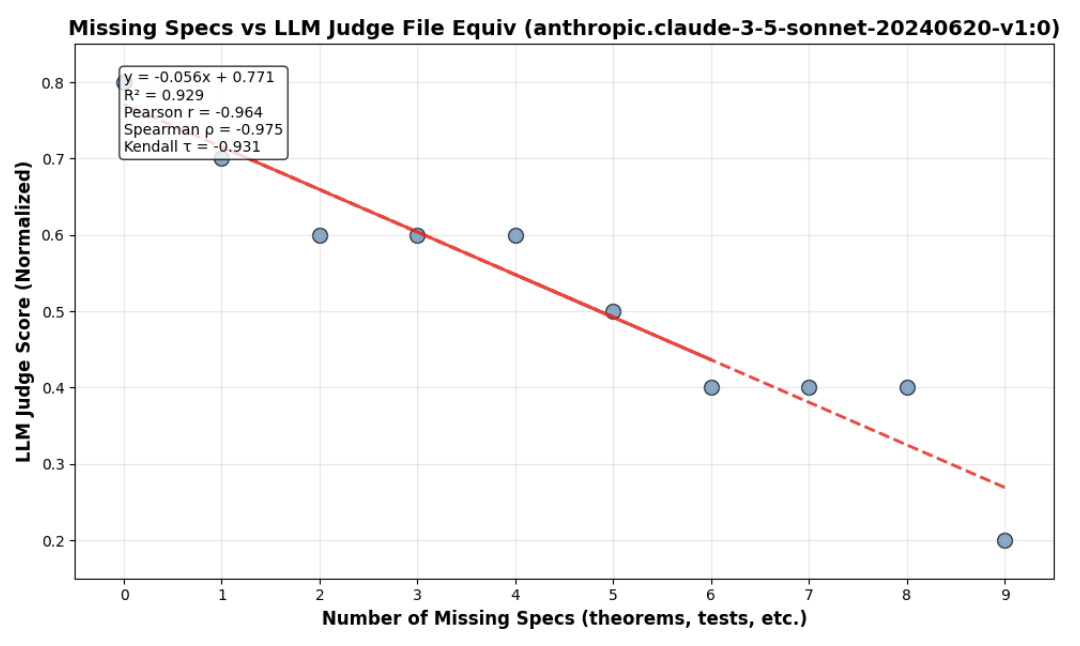
\includegraphics[width=\linewidth]{figures/3.5_specs_missing.png}
    \caption{Claude 3.5 Sonnet v1: strong monotonic decrease (\(y=-0.056x+0.771\), \(R^2=0.929\), Pearson \(r=-0.964\), Spearman \(\rho=-0.975\)).}
  \end{subfigure}\hfill
  \begin{subfigure}[t]{0.48\textwidth}
    \centering
    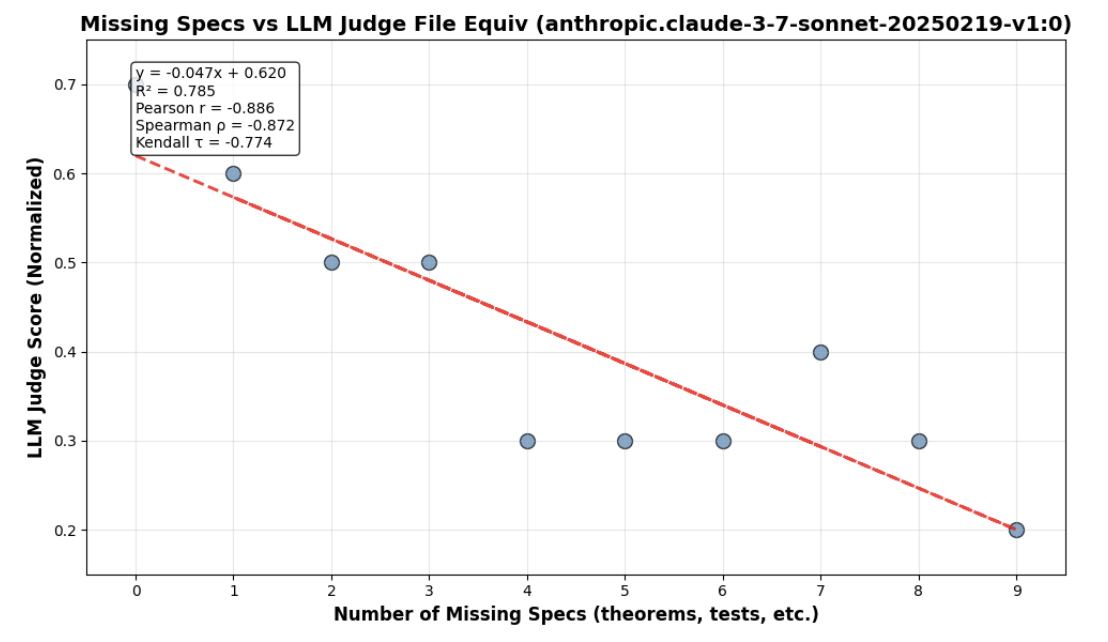
\includegraphics[width=\linewidth]{figures/3.7_specs_missing.png}
    \caption{Claude 3.7 Sonnet v1: clear negative trend with minor non-monotonicity (\(y=-0.047x+0.620\), \(R^2=0.785\), Pearson \(r=-0.886\), Spearman \(\rho=-0.872\)).}
  \end{subfigure}
  \caption{\textbf{(P3) Monotonicity w.r.t.\ missing specifications.}
    Candidate scores decrease as more theorems/tests are withheld. We retain both model variants to show robustness of the trend; 3.7’s small non-monotonicity motivated the simplified rubric used in the main results.}
  \label{fig:app-missing-specs}
\end{figure*}

\begin{figure}[t]
  \centering
  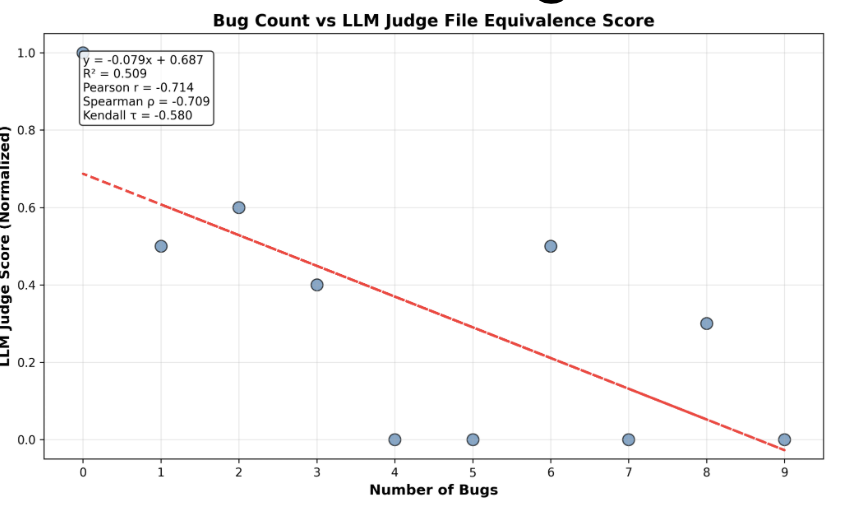
\includegraphics[width=0.85\linewidth]{figures/3.5_bugs.png}
  \caption{\textbf{(P2) Non-Monotonicity w.r.t.\ cumulative bugs (Claude 3.5 Sonnet).}
    Scores drop as more semantic bugs are injected (Pearson \(r=-0.714\), Spearman \(\rho=-0.709\), \(R^2=0.509\)); the higher noise with the initial “theorem-equivalence” prompt led us to simplify the rubric used for the final judge in the main paper.}
  \label{fig:app-bugs}
\end{figure}

\begin{figure*}[t]
  \centering
  \begin{subfigure}[t]{0.49\textwidth}
    \centering
    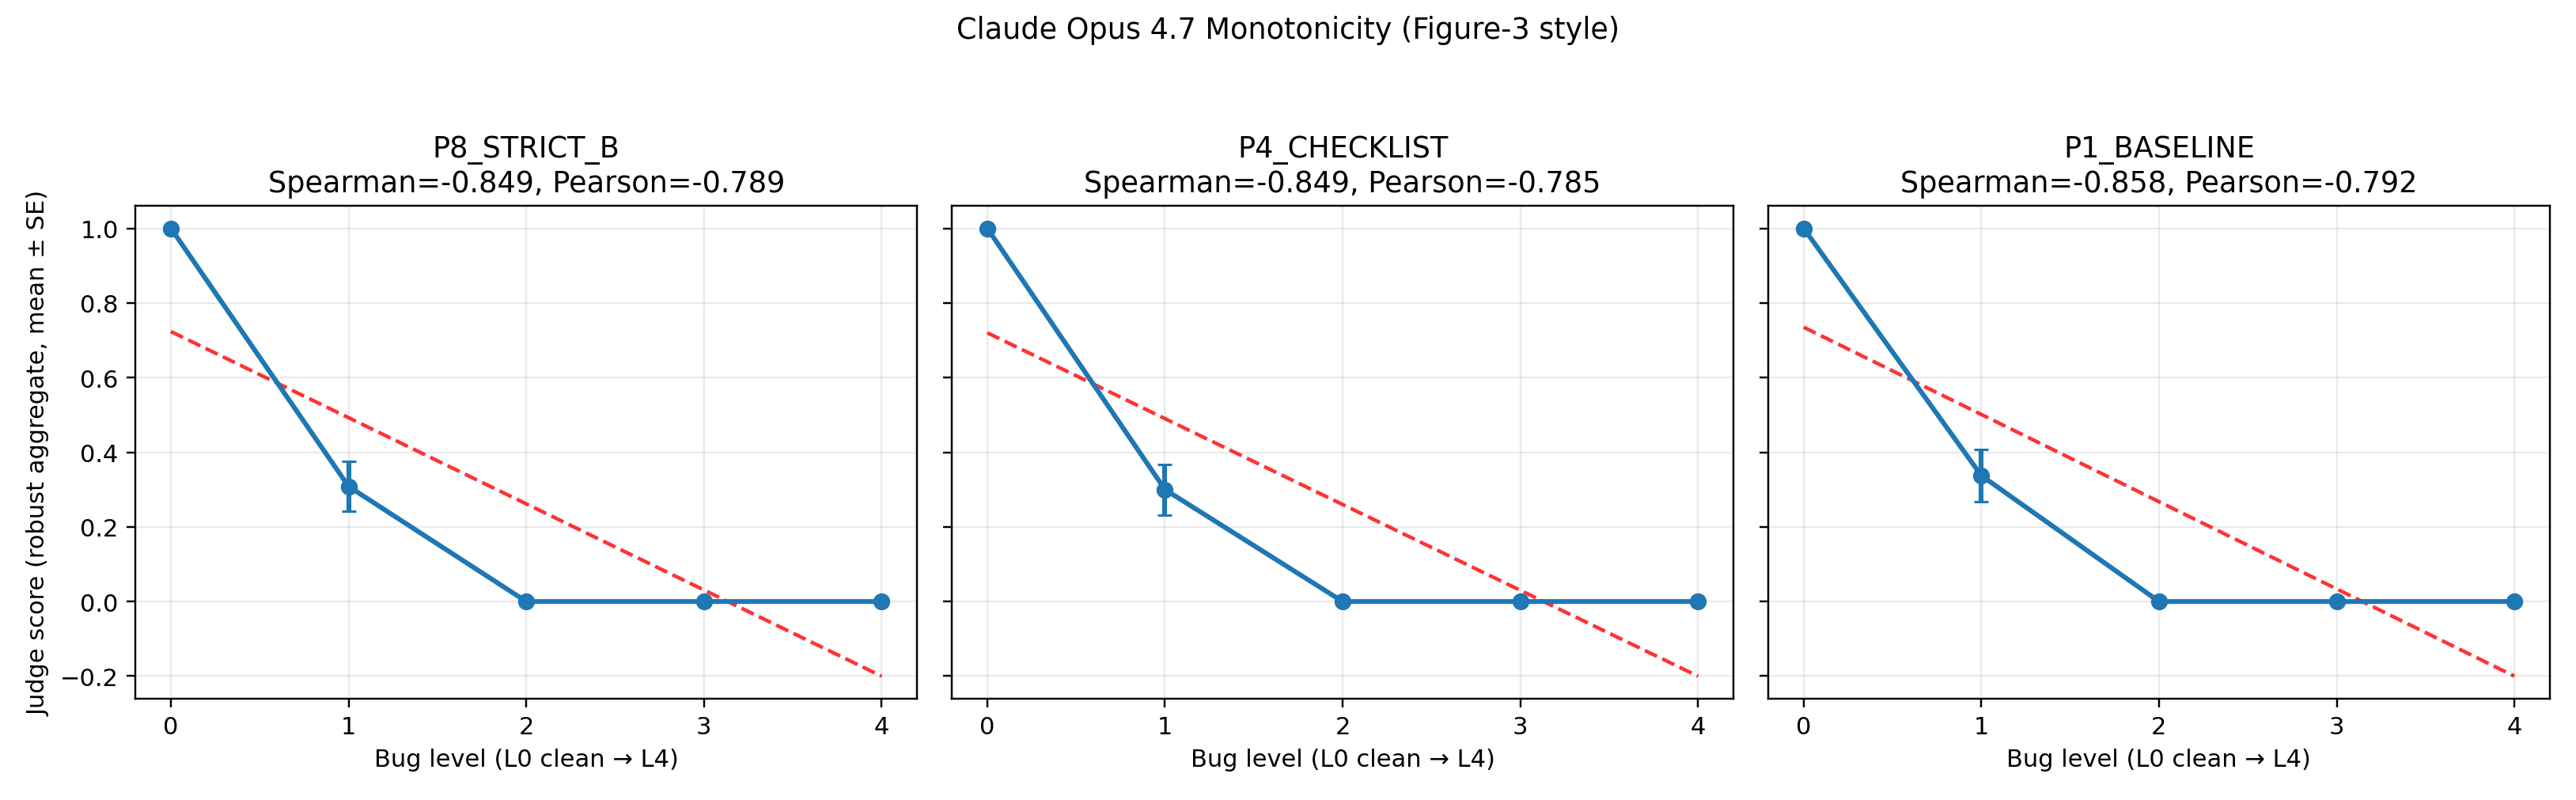
\includegraphics[width=\linewidth]{figures/fig3_style_claude_opus_monotonicity.png}
    \caption{Claude Opus 4.7 Figure-3-style monotonicity (mean \(\pm\) SE).}
  \end{subfigure}\hfill
  \begin{subfigure}[t]{0.49\textwidth}
    \centering
    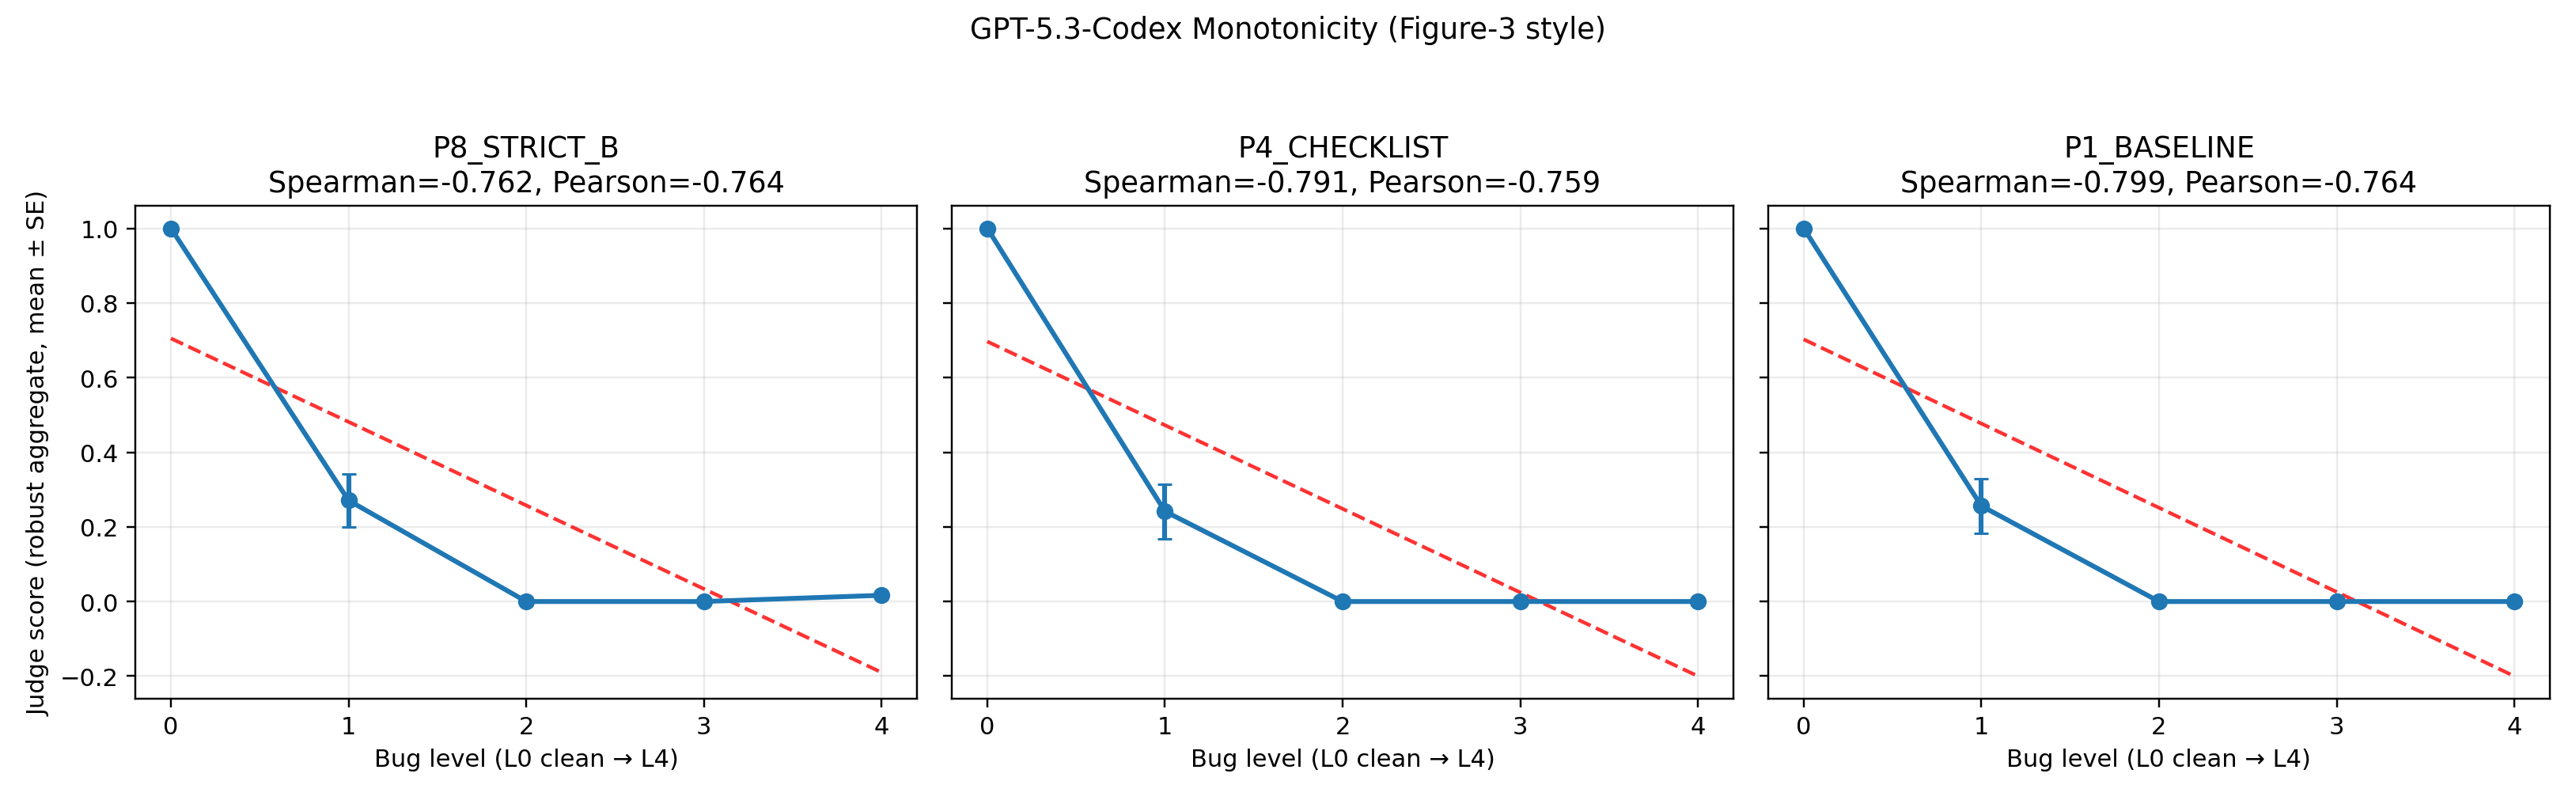
\includegraphics[width=\linewidth]{figures/fig3_style_gpt53_codex_monotonicity.png}
    \caption{GPT-5.3-Codex Figure-3-style monotonicity (mean \(\pm\) SE).}
  \end{subfigure}
  \caption{\textbf{Model-matched Figure-3-style monotonicity diagnostics.}
    Both judge families show strong monotone score degradation as bug intensity increases, under the same low-variance plotting protocol.}
  \label{fig:fig3_style_opus_codex}
\end{figure*}

\begin{figure*}[t]
  \centering
  \begin{subfigure}[t]{0.49\textwidth}
    \centering
    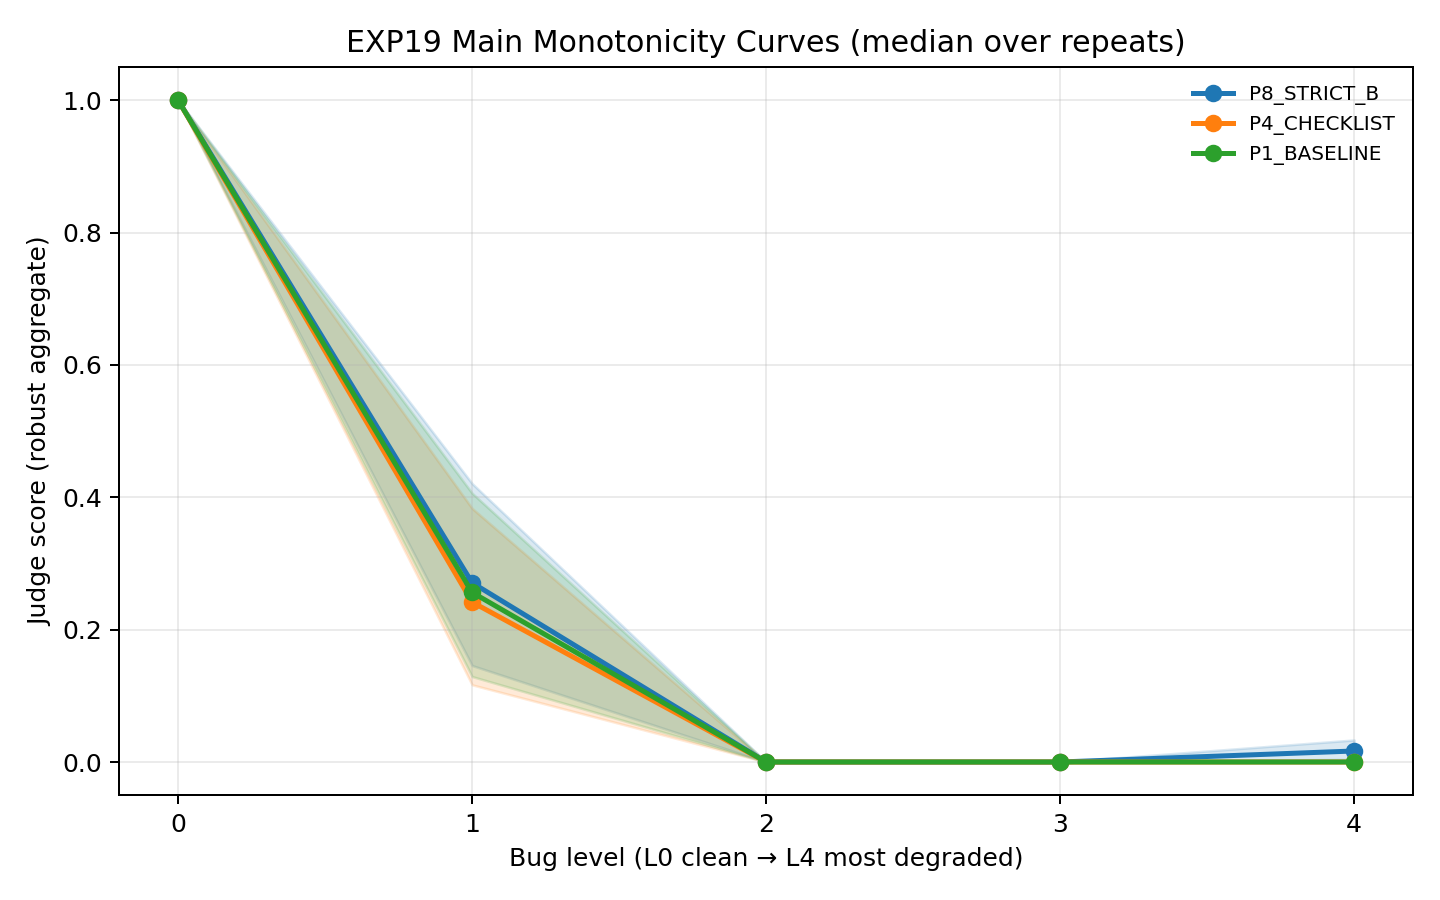
\includegraphics[width=\linewidth]{figures/fig_main_monotonicity_lowvar_codex.png}
    \caption{Codex low-variance monotonicity curves.}
  \end{subfigure}\hfill
  \begin{subfigure}[t]{0.49\textwidth}
    \centering
    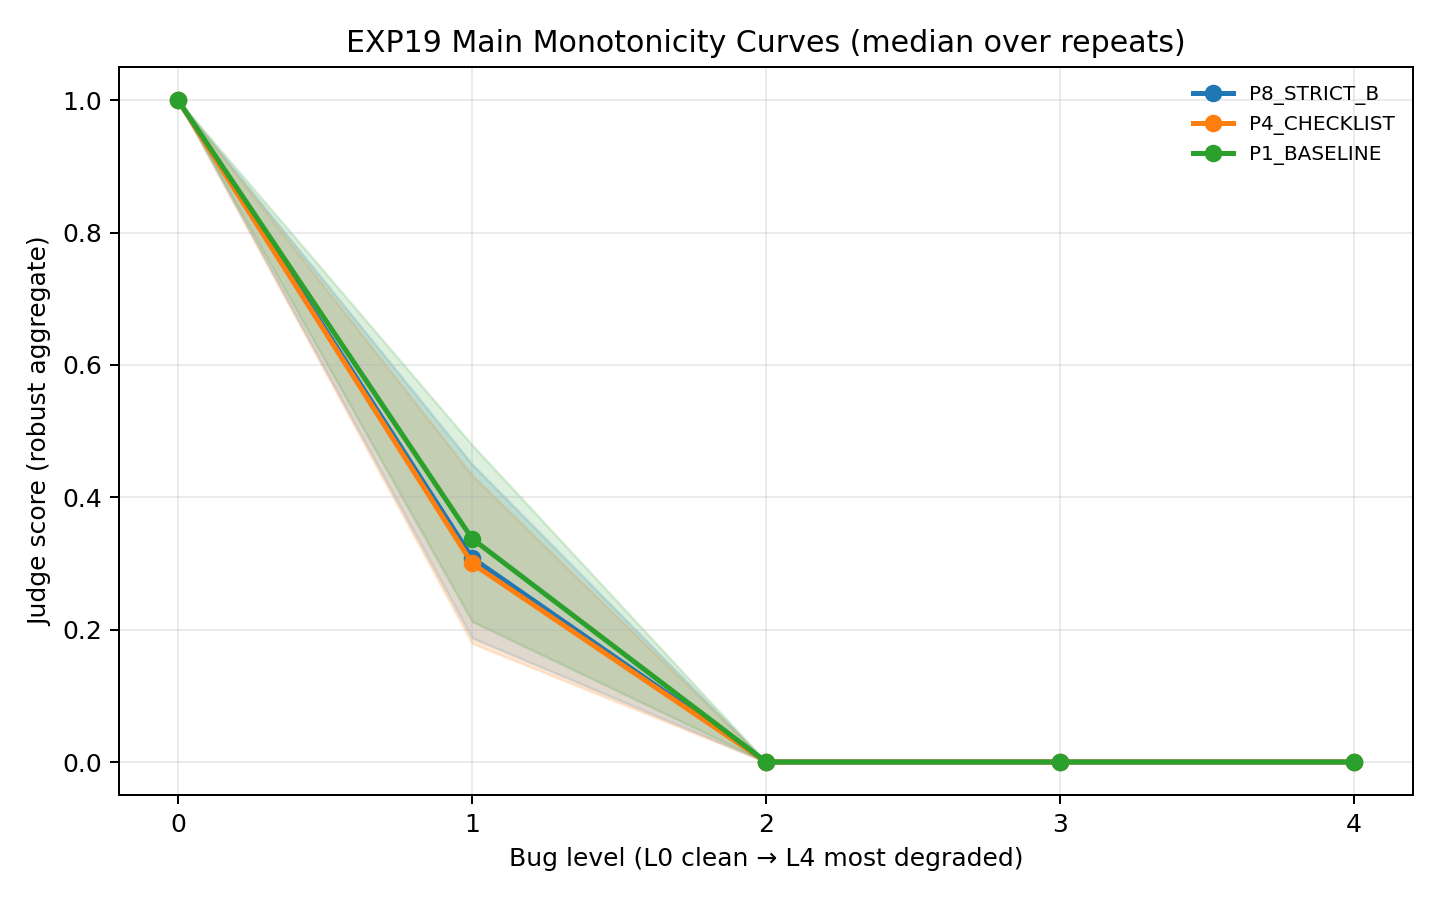
\includegraphics[width=\linewidth]{figures/fig_main_monotonicity_lowvar_opus47.png}
    \caption{Opus 4.7 low-variance monotonicity curves.}
  \end{subfigure}
  \caption{\textbf{Low-variance monotonicity trends across model families.}
    Both judge families show strong non-increasing behavior as bug intensity increases, under robust repeat aggregation.}
  \label{fig:lowvar_mono_codex_opus}
\end{figure*}

\section{Validation-Set Human Alignment Appendix}\label{app:exp16-exp17}
This appendix reports full visual diagnostics for Exp16/Exp17 under final robust settings (three validation label sets: pass1, pass2, avg).

\begin{figure}[t]
  \centering
  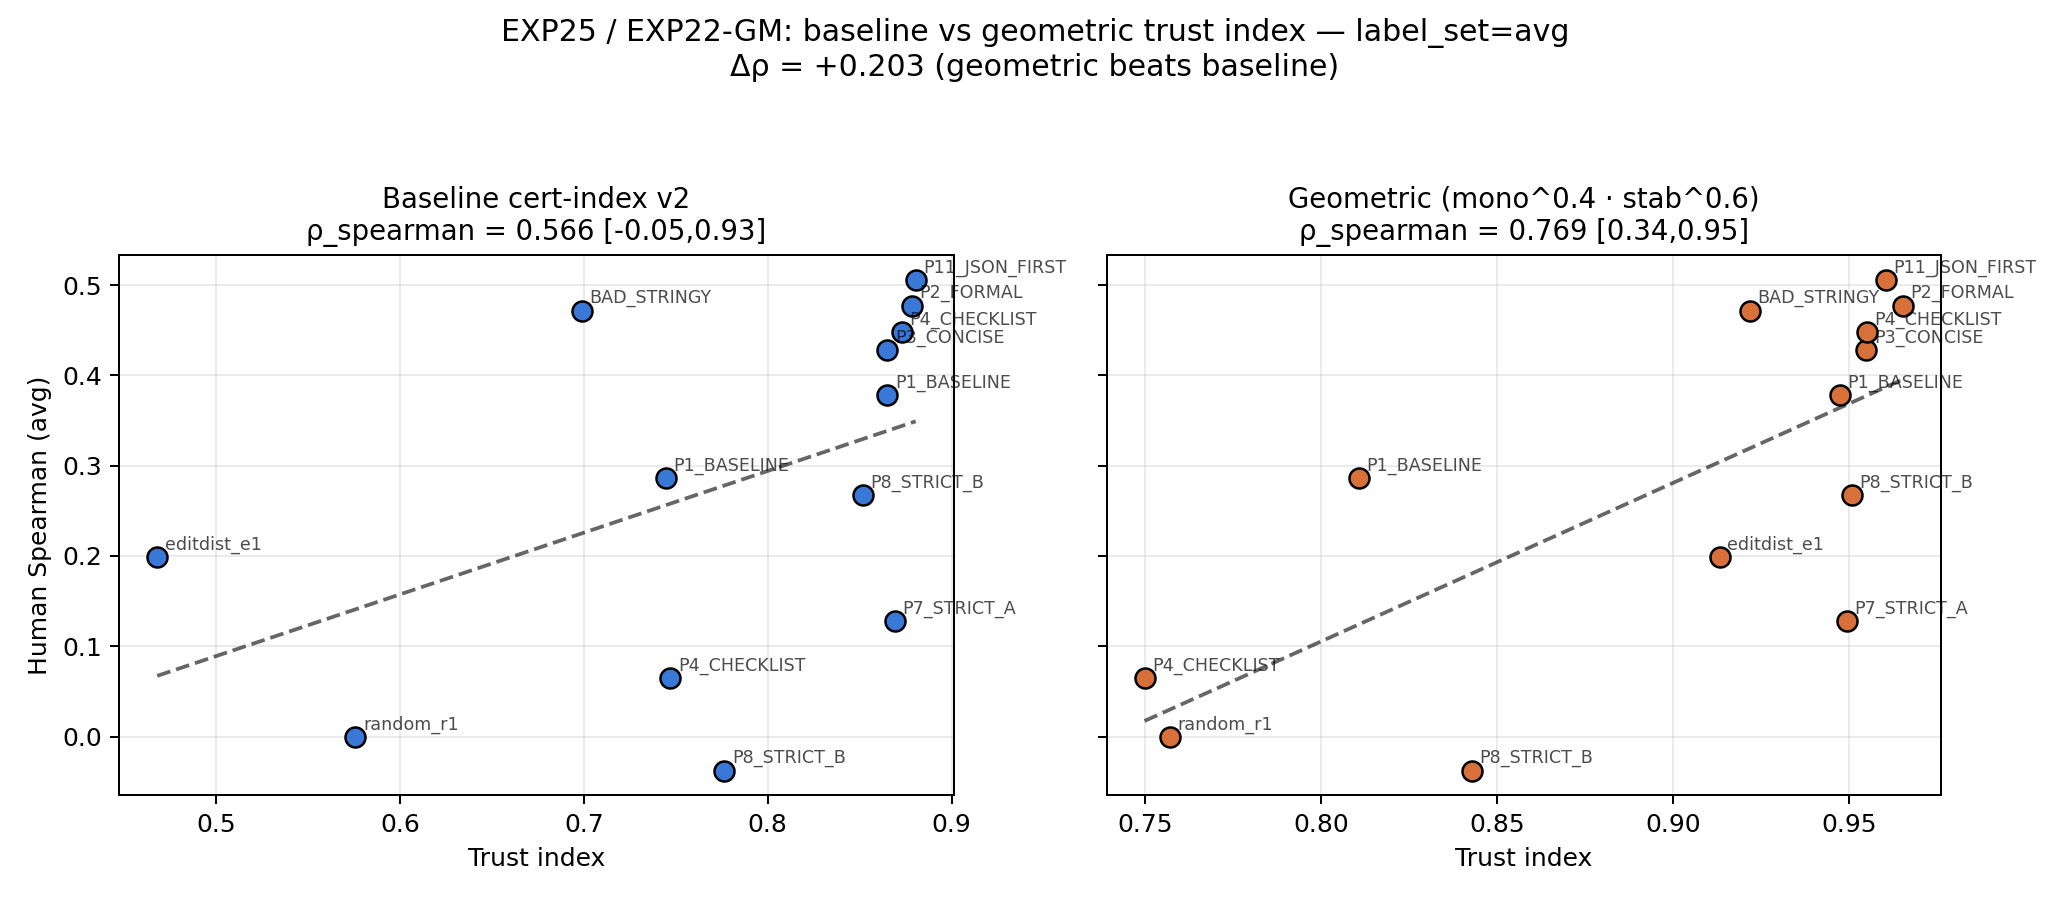
\includegraphics[width=\linewidth]{figures/fig7_trend_update_baseline_vs_geom_13judge_avg.png}
  \caption{\textbf{Appendix: Expanded 13-judge panel trend (avg validation labels).}
    Geometric trust index retains strong alignment with human correlation at larger judge-panel size (\(\rho=0.769\));
    pass-specific values are pass1 \(\rho=0.764\), pass2 \(\rho=0.753\).}
  \label{fig:app-exp25-13judge}
\end{figure}

\begin{figure*}[t]
  \centering
  \begin{subfigure}[t]{0.32\textwidth}
    \centering
    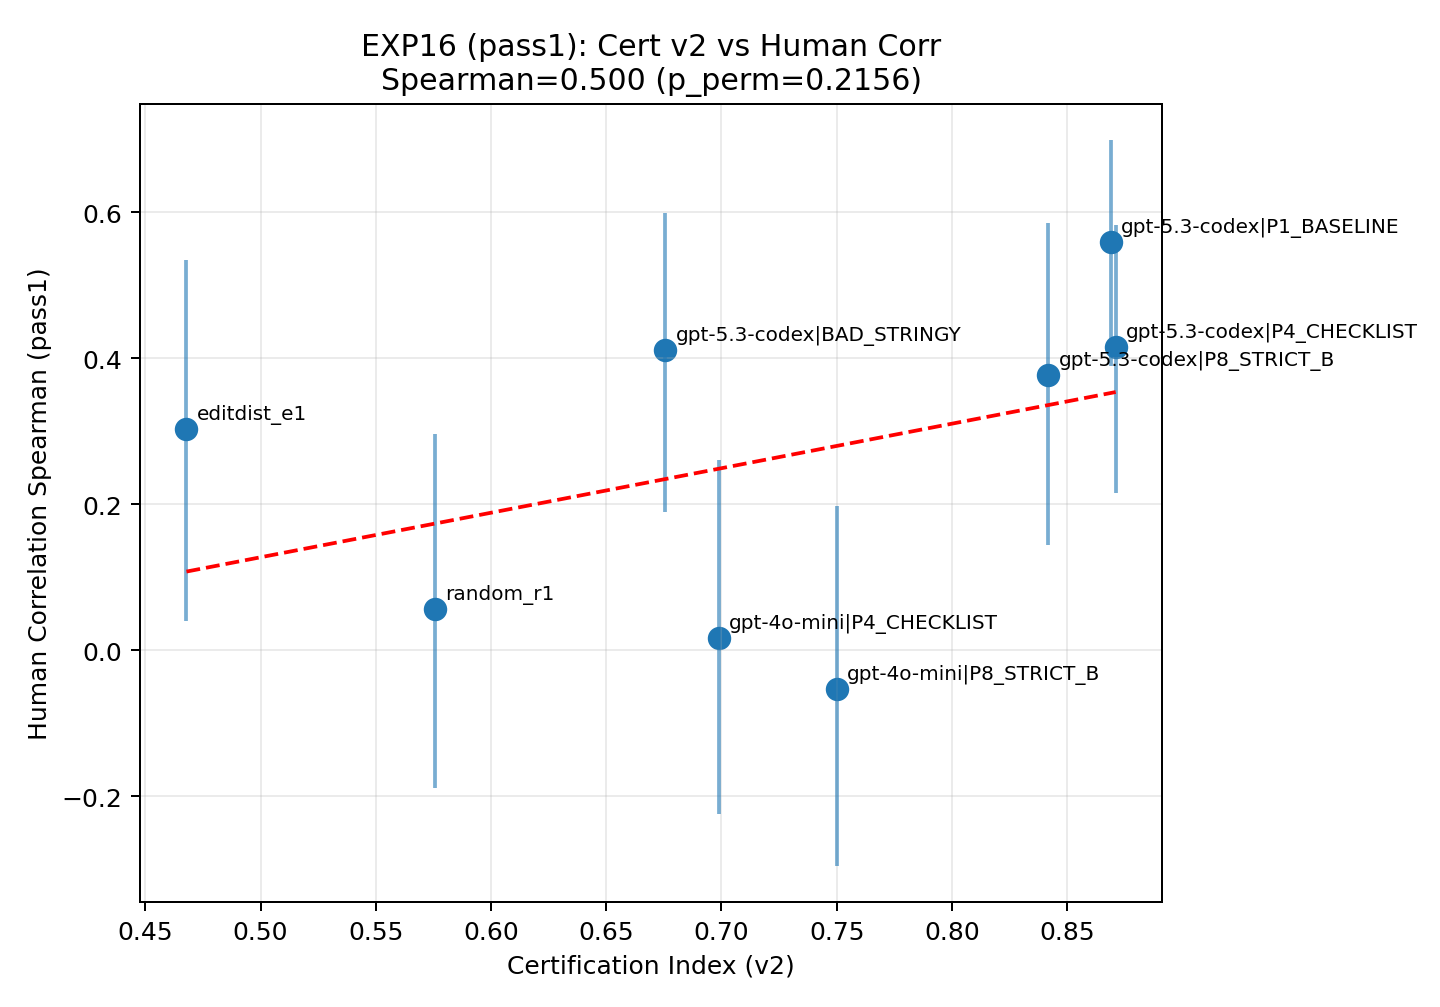
\includegraphics[width=\linewidth]{figures/exp16_final_robust/fig_cert_vs_human_scatter_pass1.png}
    \caption{Exp16 trend (pass1)}
  \end{subfigure}\hfill
  \begin{subfigure}[t]{0.32\textwidth}
    \centering
    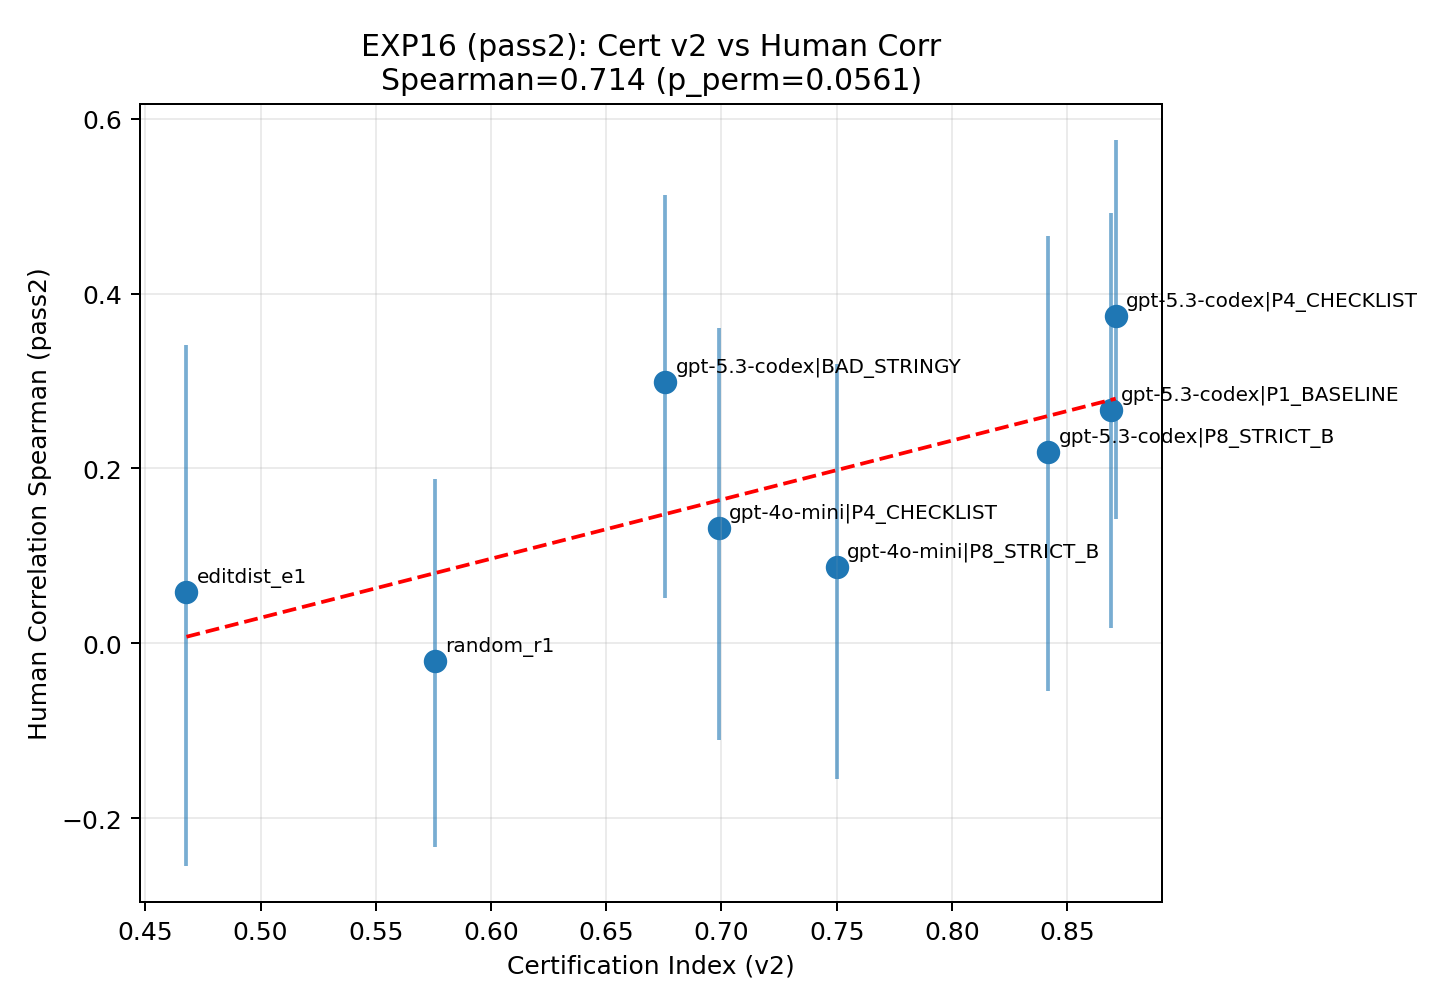
\includegraphics[width=\linewidth]{figures/exp16_final_robust/fig_cert_vs_human_scatter_pass2.png}
    \caption{Exp16 trend (pass2)}
  \end{subfigure}\hfill
  \begin{subfigure}[t]{0.32\textwidth}
    \centering
    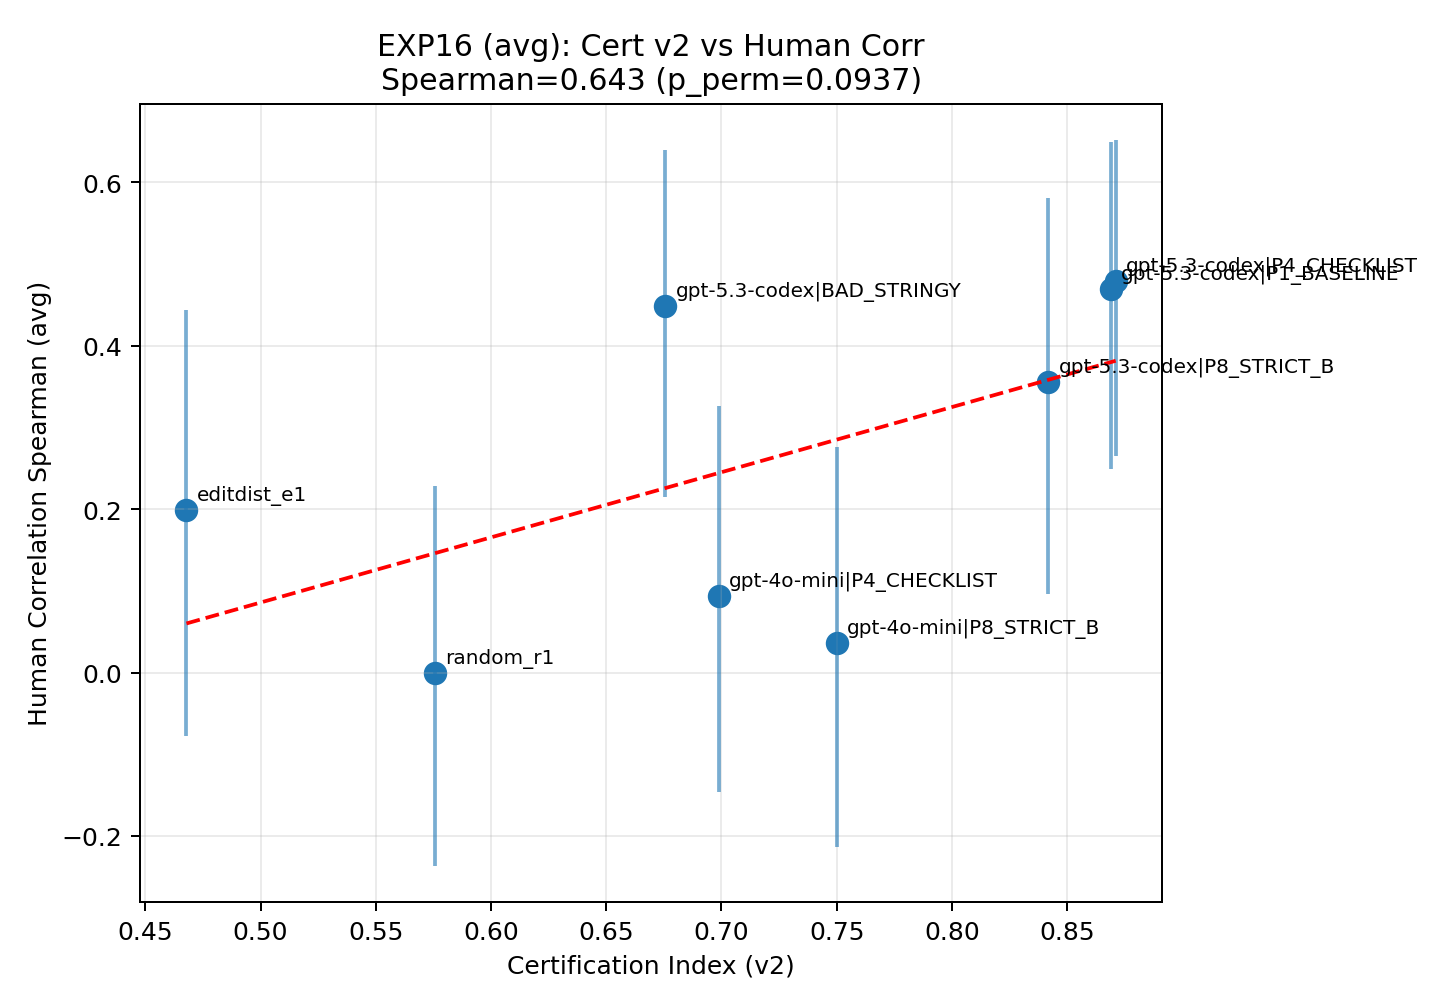
\includegraphics[width=\linewidth]{figures/exp16_final_robust/fig_cert_vs_human_scatter_avg.png}
    \caption{Exp16 trend (avg)}
  \end{subfigure}
  \caption{\textbf{Judge-level JTI-to-validation trend across all validation label sets (Exp16).}
    The strongest and most stable effect is for trend-v1 JTI, with averaged labels giving the largest effect size.}
  \label{fig:app-exp16-all}
\end{figure*}

\begin{figure*}[t]
  \centering
  \begin{subfigure}[t]{0.32\textwidth}
    \centering
    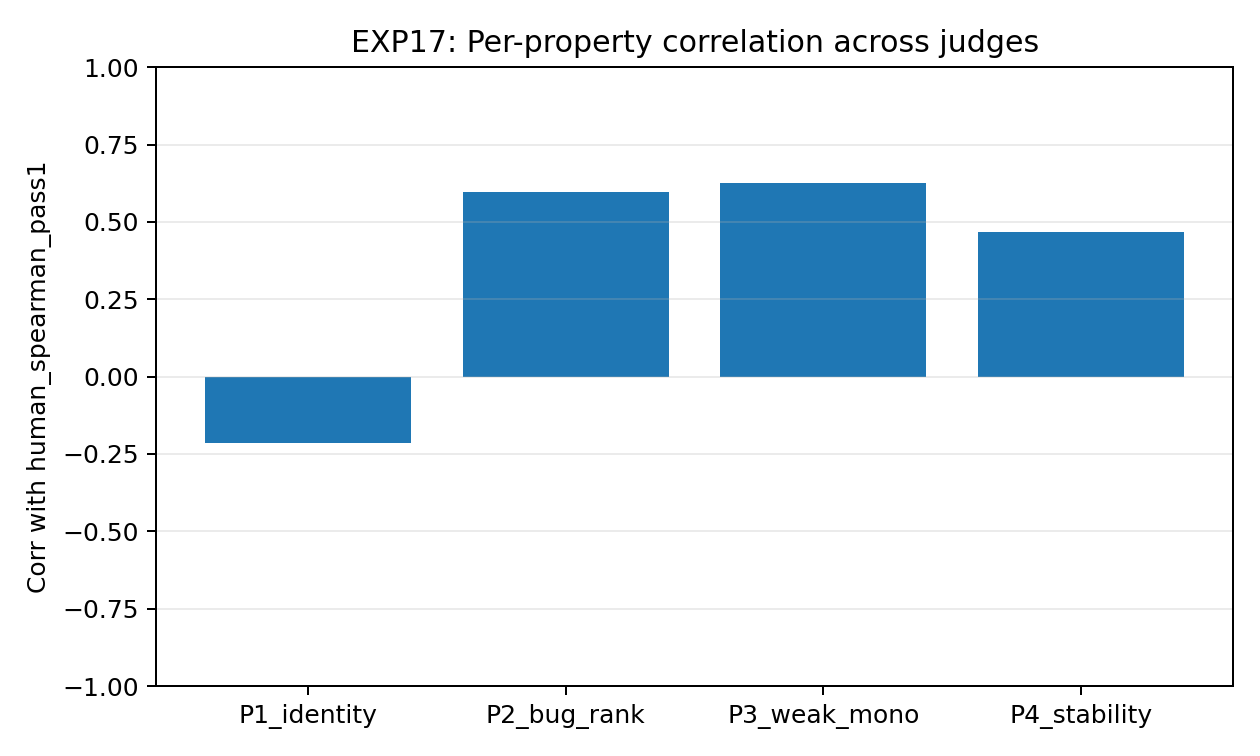
\includegraphics[width=\linewidth]{figures/exp17_final_robust/fig_property_vs_human_bars_pass1.png}
    \caption{Exp17 per-property (pass1)}
  \end{subfigure}\hfill
  \begin{subfigure}[t]{0.32\textwidth}
    \centering
    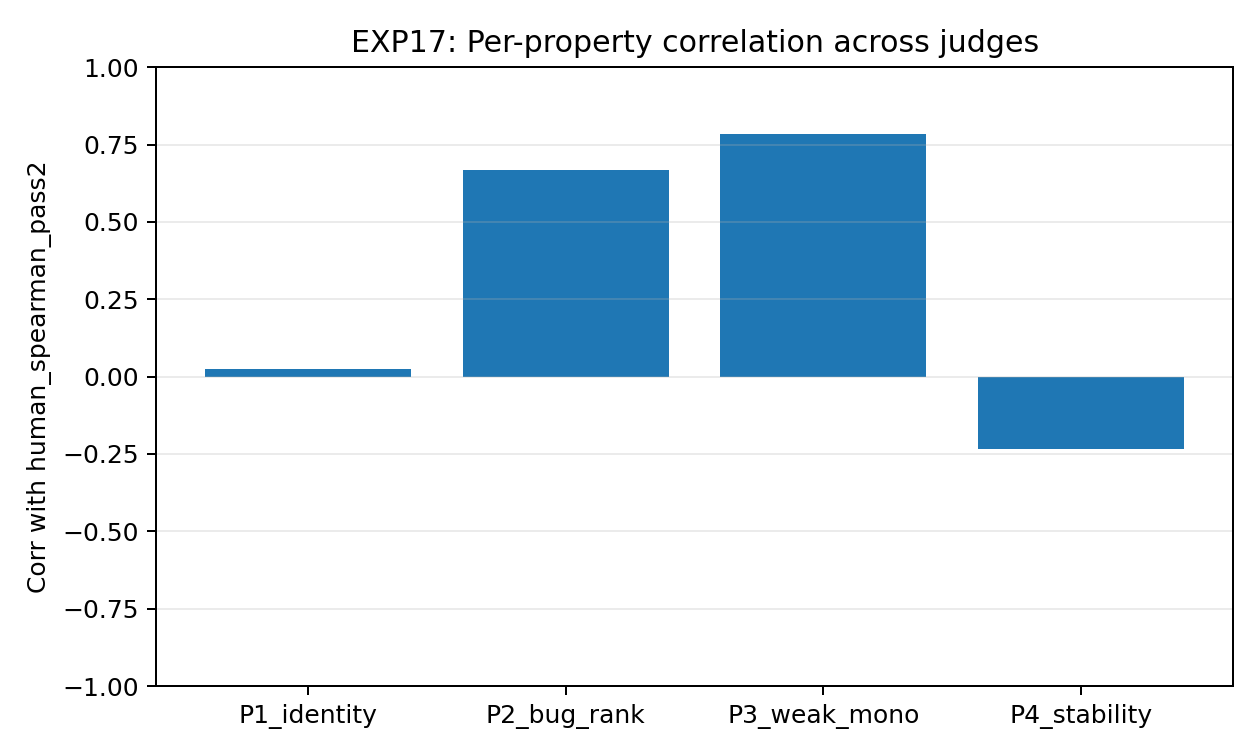
\includegraphics[width=\linewidth]{figures/exp17_final_robust/fig_property_vs_human_bars_pass2.png}
    \caption{Exp17 per-property (pass2)}
  \end{subfigure}\hfill
  \begin{subfigure}[t]{0.32\textwidth}
    \centering
    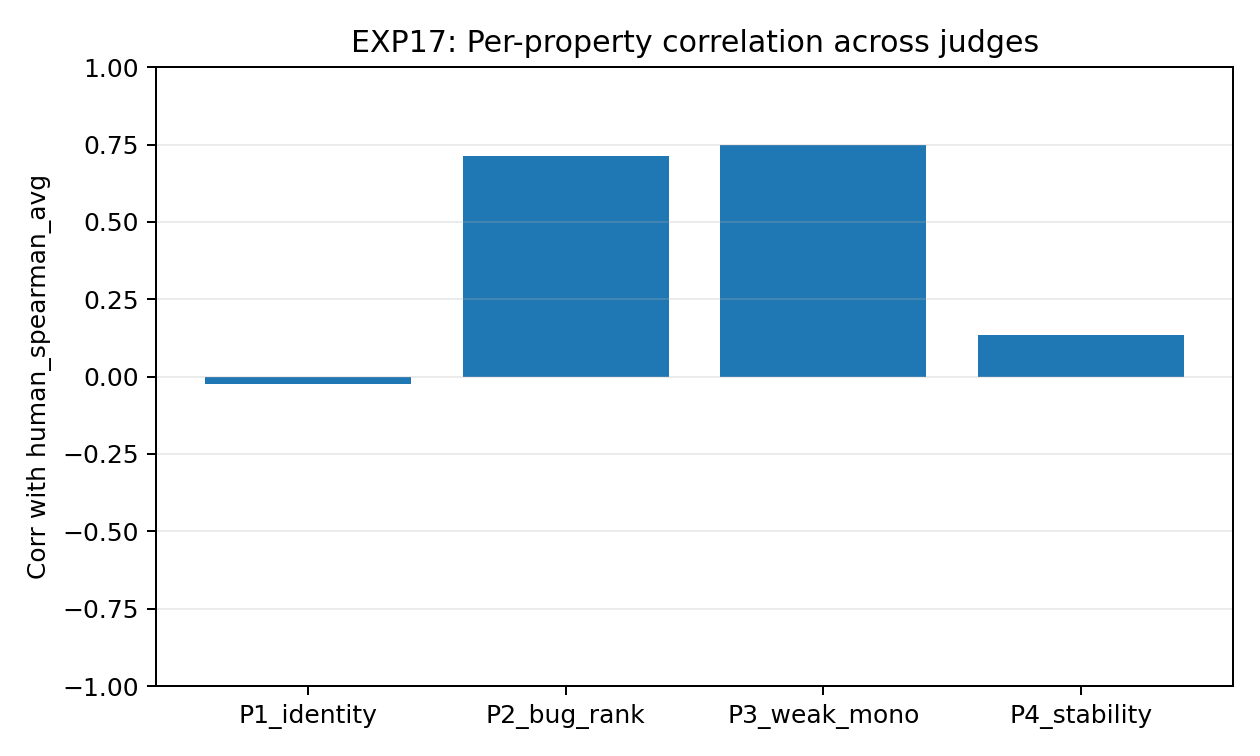
\includegraphics[width=\linewidth]{figures/exp17_final_robust/fig_property_vs_human_bars_avg.png}
    \caption{Exp17 per-property (avg)}
  \end{subfigure}
  \caption{\textbf{Property-wise validation-set human-alignment diagnostics (Exp17).}
    P3 weak monotonicity is consistently the strongest predictor across label sets; P2 is second strongest; P1/P4 are weaker as standalone predictors at this scale.}
  \label{fig:app-exp17-all}
\end{figure*}

\begin{figure}[t]
  \centering
  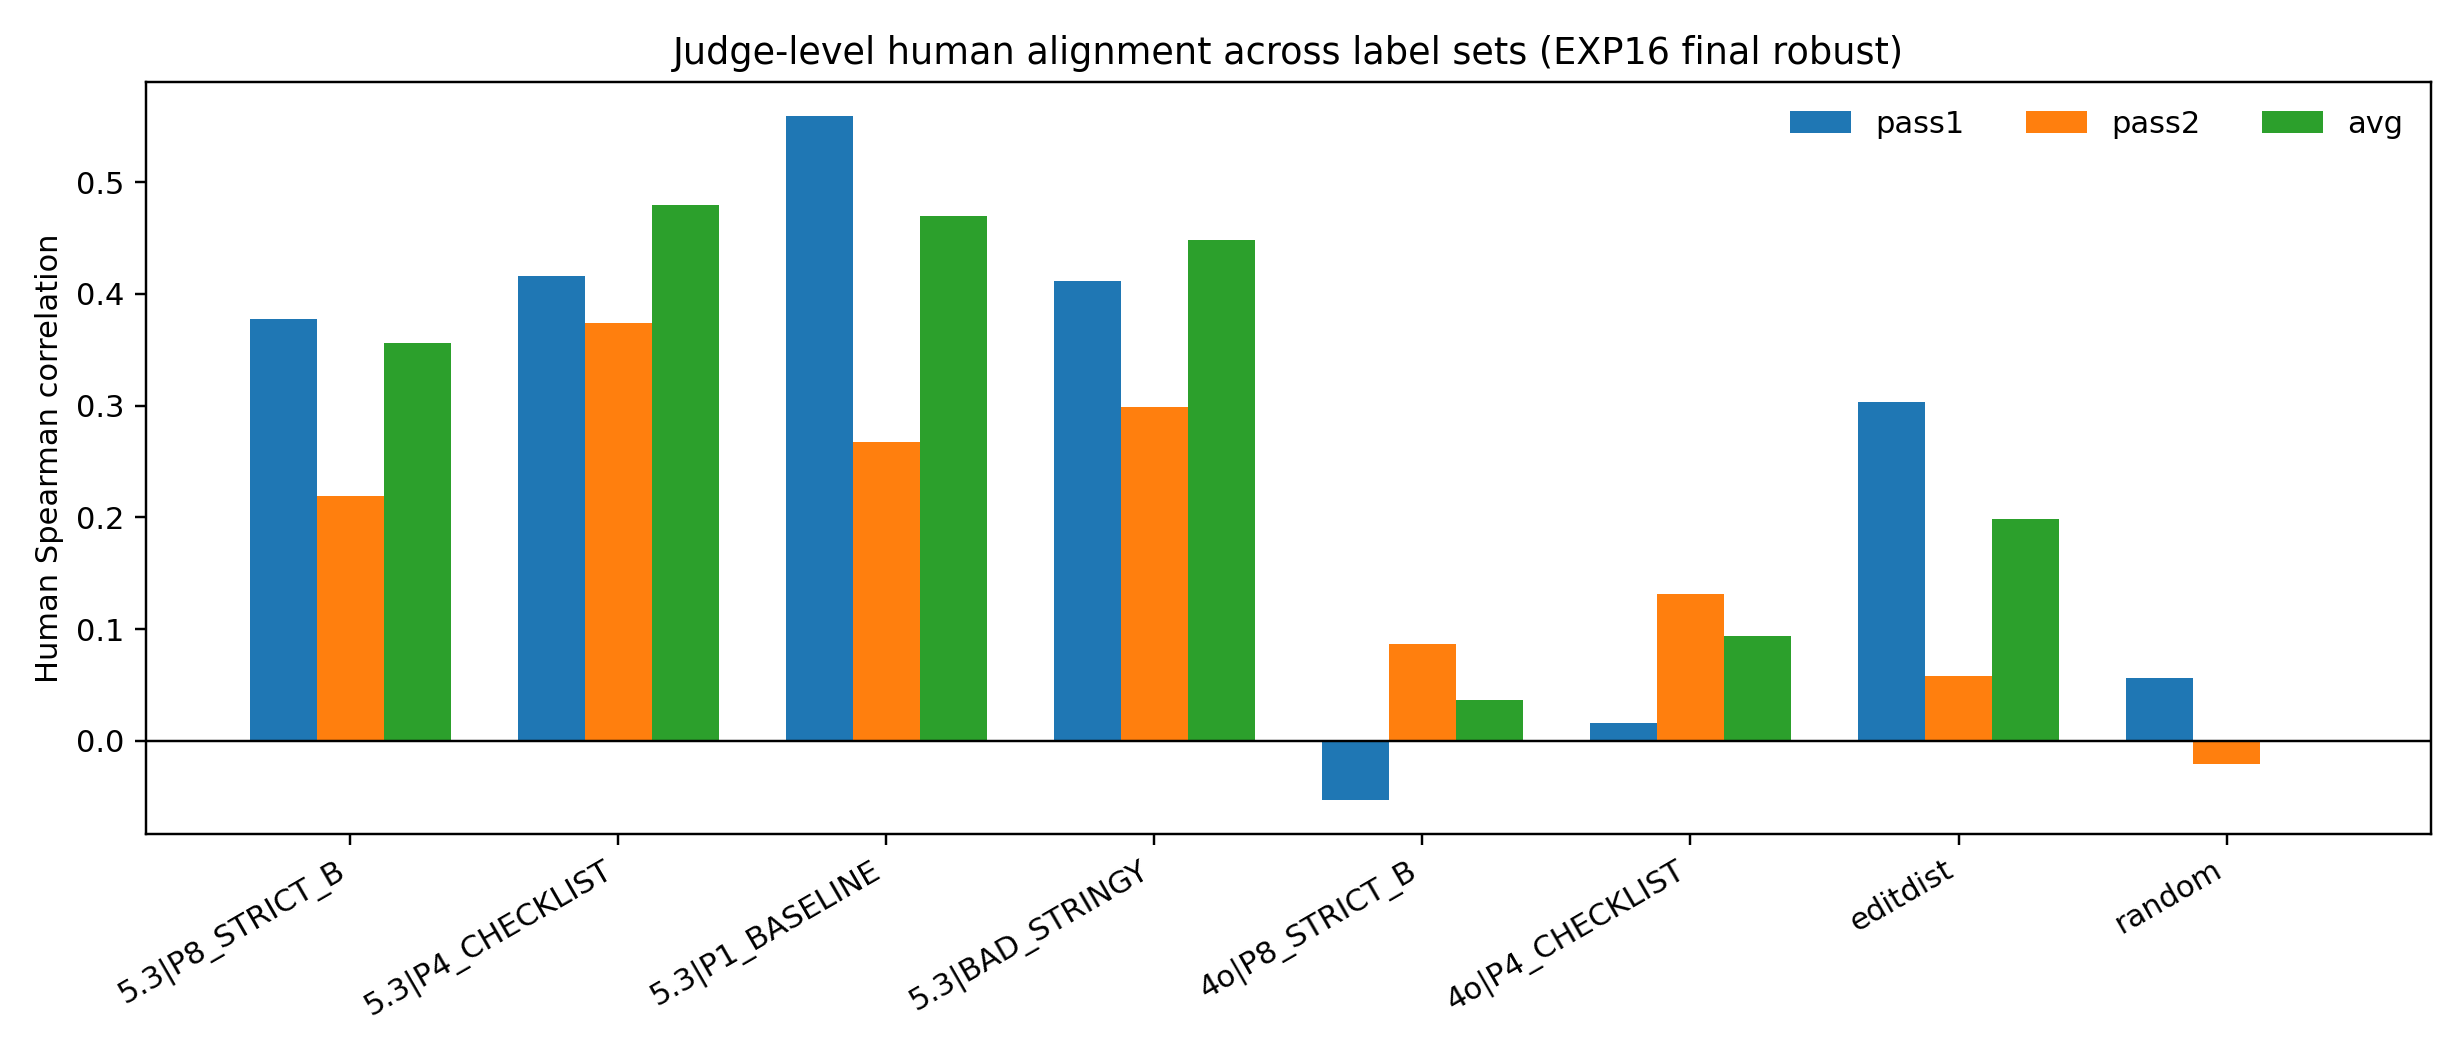
\includegraphics[width=\linewidth]{figures/exp16_final_robust/fig_human_corr_by_judge_and_labelset.png}
  \caption{\textbf{Unplotted diagnostic added for this version:} judge-wise validation-set human Spearman across pass1/pass2/avg.
    GPT-5.3-Codex variants remain above weaker baselines on most label sets; pass-to-pass variation is visible and motivates reporting all three label sets.}
  \label{fig:app-judge-labelset-bars}
\end{figure}

\subsection{Naive Codex-Style Blind Baseline}
To contextualize JTI-ranked judge performance, we evaluate a naive blind baseline on the same pair set (\(n=72\) overlap), using a single-pass, surface-form-oriented Codex-style rubric without property-calibration constraints (no monotonicity/stability calibration).
The baseline tracks pass2 labels somewhat but remains substantially weaker and less consistent than the top JTI-ranked judges, especially on pass1 and in absolute error.

\begin{table}[t]
  \centering
  \small
  \begin{tabular}{lcccc}
    \toprule
    \textbf{Label Set} & \(\rho_s\)                      & \(r\)                           & \(\tau\)                        & \textbf{MAE} \\
    \midrule
    pass1              & 0.171 (\(p=0.151\))             & 0.218 (\(p=0.0656\))            & 0.155 (\(p=0.144\))             & 1.049        \\
    pass2              & 0.388 (\(p=7.58\times10^{-4}\)) & 0.427 (\(p=1.87\times10^{-4}\)) & 0.343 (\(p=9.40\times10^{-4}\)) & 1.333        \\
    \bottomrule
  \end{tabular}
  \caption{\textbf{Naive blind baseline vs.\ validation labels (0--5 scale).}
    \(\rho_s\): Spearman, \(r\): Pearson, \(\tau\): Kendall; MAE is absolute error on the 0--5 scale.
    This baseline is included as a sanity-check negative control and is not used for final ranking claims.}
  \label{tab:app-naive-blind-baseline}
\end{table}

\subsection{Human-Human Agreement Ceiling Context}
Validation-set judge-human Spearman values should be interpreted relative to the reliability of human labels themselves.
Across Ethan pass1 vs pass2 on the aligned set (\(n=72\)), inter-pass agreement is moderate (Spearman \(0.249\), Pearson \(0.375\), Kendall \(0.221\), QWK \(0.372\)).
Thus, validation-set judge-human Spearman values in the \(0.48\)--\(0.56\) range are non-trivial and should be interpreted as approaching the available annotation ceiling in this dataset rather than as ``low absolute'' values.

\begin{table}[t]
  \centering
  \small
  \begin{tabular}{lcc}
    \toprule
    \textbf{Quantity}                           & \textbf{Value} & \textbf{Notes}                      \\
    \midrule
    Human-human Spearman (pass1 vs pass2)       & 0.249          & \(95\%\ \text{CI}=[-0.015, 0.489]\) \\
    Human-human Pearson (pass1 vs pass2)        & 0.375          & \(95\%\ \text{CI}=[0.076, 0.604]\)  \\
    Human-human QWK (pass1 vs pass2)            & 0.372          & \(95\%\ \text{CI}=[0.073, 0.581]\)  \\
    Human-human MAE (pass1 vs pass2)            & 0.778          & On aligned \(n=72\), 0--5 rubric    \\
    Human-human MSE (pass1 vs pass2)            & 1.139          & On aligned \(n=72\), 0--5 rubric    \\
    JS divergence (pass1 vs pass2)              & 0.081 bits     & Symmetric histogram divergence      \\
    KL\((\text{pass1}\Vert\text{pass2})\)       & 0.415 bits     & Asymmetric divergence               \\
    Best validation-set Spearman (avg labels)   & 0.480          & GPT-5.3-Codex P4\_CHECKLIST         \\
    Best validation-set Spearman (pass1 labels) & 0.559          & GPT-5.3-Codex P1\_BASELINE          \\
    \bottomrule
  \end{tabular}
  \caption{\textbf{Human-human agreement ceiling context.}
    Inter-pass human agreement is moderate, and inter-pass dispersion (MAE/divergence) is non-zero, so validation-set judge-human values near \(0.5\) are meaningful on this benchmark and should be interpreted with label-noise context.}
  \label{tab:app-human-human-ceiling}
\end{table}

\begin{figure}[t]
  \centering
  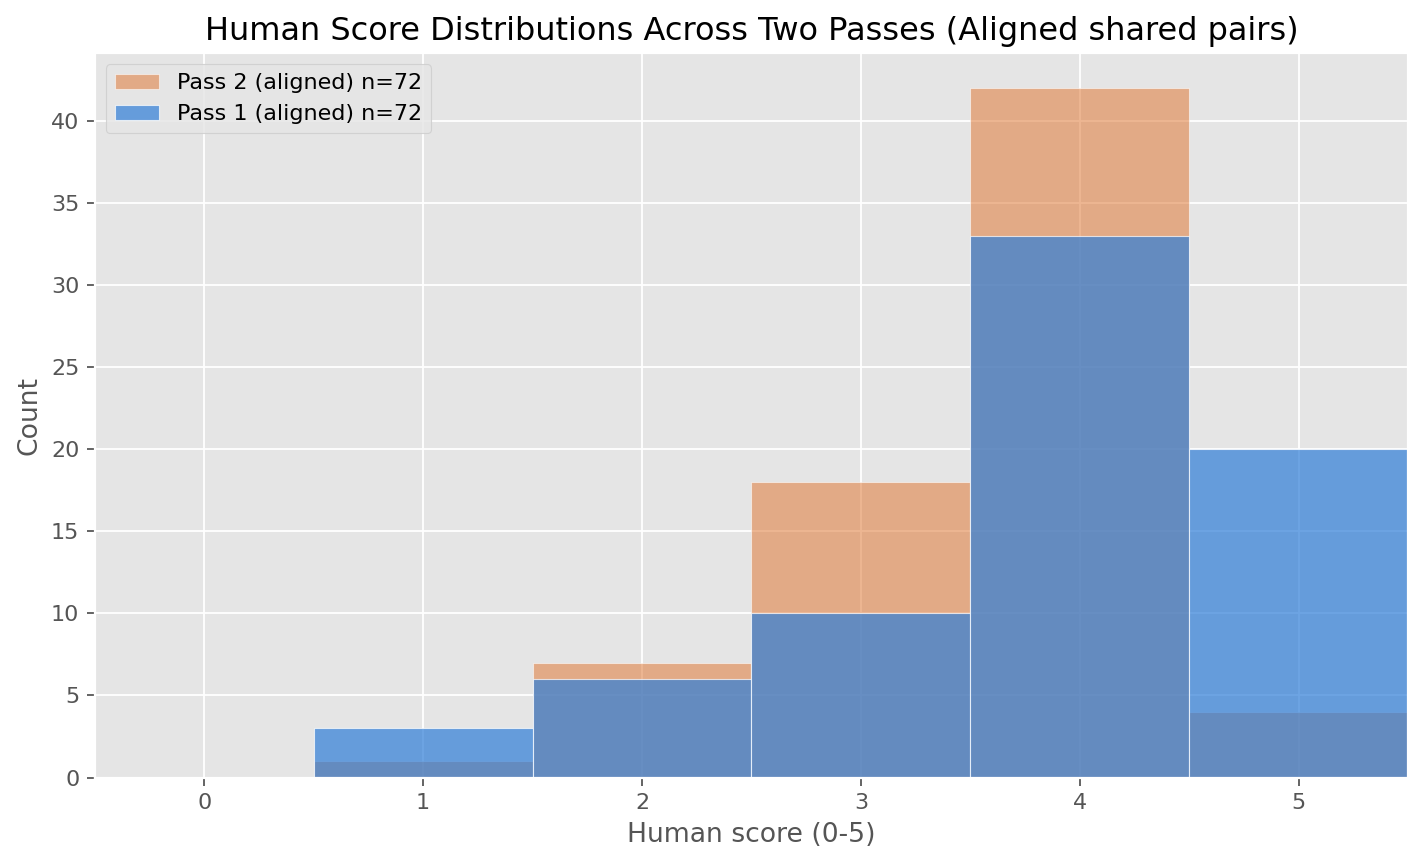
\includegraphics[width=\linewidth]{figures/hist_human_scores_two_passes_aligned72_0to5.png}
  \caption{\textbf{Human-score dispersion across passes (aligned \(n=72\), 0--5 scale).}
    Overlaid pass1/pass2 histograms show visible distribution shift, consistent with the non-zero MAE/MSE and divergence statistics in Table~\ref{tab:app-human-human-ceiling}.}
  \label{fig:app-human-pass-hist}
\end{figure}

\subsection{Cross-Model Validation Status (Full vs Preliminary)}
To avoid over-claiming, we separate full-scale and preliminary evidence.
Main conclusions in this paper use full-scale runs only (Exp16/Exp17: \(n=8\) judges, \(n=72\) aligned rows, pass1/pass2/avg label sets).
Claude Sonnet certification is currently preliminary (\(3\) files) and is included as directional evidence only, not as a core statistical pillar.

\begin{table}[t]
  \centering
  \small
  \begin{tabular}{@{}p{0.30\linewidth}p{0.14\linewidth}p{0.13\linewidth}p{0.27\linewidth}@{}}
    \toprule
    \textbf{Judge Setup}             & \textbf{Scale}       & \makecell[c]{\textbf{In Main}                                 \\\textbf{Claims}} & \textbf{Role} \\
    \midrule
    GPT-5.3-Codex prompts (P8/P4/P1) & Full VeriBench pairs & Yes                           & Primary JTI-ranked judges     \\
    GPT-5.3-Codex BAD\_STRINGY       & Full VeriBench pairs & Yes                           & Same-model stress baseline    \\
    Qwen3-Coder prompts (P8/P4/P1)   & Full VeriBench pairs & Yes                           & Open-weights cross-family run \\
    Qwen3-Coder BAD\_STRINGY         & Full VeriBench pairs & Yes                           & Open-weights stress baseline  \\
    GPT-4o-mini prompts (P8/P4)      & Full VeriBench pairs & Yes                           & Cross-family baseline         \\
    Edit-distance / random baselines & Full VeriBench pairs & Yes                           & Non-LLM controls              \\
    Claude Sonnet certification run  & 3 files (prelim)     & No                            & Directional cross-model check \\
    \bottomrule
  \end{tabular}
  \caption{\textbf{Cross-model validation status.}
    This paper's inferential claims are grounded in full-scale runs; Claude results are explicitly preliminary and not used as primary evidence.}
  \label{tab:app-cross-model-status}
\end{table}

\subsection{Leanstral Negative-Control Reaggregation (AM/GM/Variance-Aware)}
To stress-test whether index choice alone can ``rescue'' a weak judge family, we re-aggregate the same Leanstral Exp16 outputs under three indices:
\[
  \mathrm{AM}=\text{cert\_index\_v2} \quad \text{(arithmetic baseline)},
\]
\[
  \mathrm{GM}=\mathrm{mono}^{0.4}\cdot \mathrm{stab}^{0.6},
\]
\[
  \mathrm{TI}_{\mathrm{var}}=\exp\!\Big(\tfrac{1}{3}\log C_f+\tfrac{1}{3}\log(1-\widetilde{\mathrm{VarCorr}})+\tfrac{1}{3}\log(1-\widetilde{\mathrm{VarScore}})\Big),
\]
where \(C_f\) is the mean per-file property-correlation quality term, and \(\widetilde{\mathrm{VarCorr}},\widetilde{\mathrm{VarScore}}\) are normalized variance penalties (lower is better before \(1-\cdot\)).
We report Spearman between index score and validation-set human Spearman across judges.

\begin{table}[t]
  \centering
  \small
  \begin{tabular}{lccc}
    \toprule
    \textbf{Label Set} & \textbf{AM (v2)} & \textbf{GM} & \textbf{Variance-Aware \(\mathrm{TI}_{\mathrm{var}}\)} \\
    \midrule
    val (pass1)        & -0.5952          & -0.1429     & -0.1190                                                \\
    test (pass2)       & -0.1905          & -0.2619     & -0.0476                                                \\
    avg                & -0.4286          & -0.2143     & -0.0952                                                \\
    \bottomrule
  \end{tabular}
  \caption{\textbf{Leanstral remains low-alignment under multiple index constructions.}
    Re-aggregation improves over the arithmetic baseline in some splits, but all three settings remain near-zero or negative.
    This suggests the bottleneck is likely the underlying judge behavior for this ranking task (human-preference alignment), not only index form.
    One plausible hypothesis is that Leanstral is stronger for Lean proof editing/generation than for calibrated pairwise judging under this rubric; we treat this as a testable conjecture, not a final causal claim.}
  \label{tab:app-leanstral-index-reagg}
\end{table}

\subsection{Failure Modes Found by Certification (Not Hidden)}
The certification framework is useful precisely because it identifies failures:
\textbf{(i) alpha-renaming sensitivity} is the dominant identity/invariance gap,
and \textbf{(ii) local bug-ladder reversals} occur despite overall negative monotone trends.
We therefore report both strengths and weaknesses, and include alpha-ablation diagnostics.
On trend-v1 Spearman (JTI \(\rightarrow\) validation-set human Spearman), excluding alpha variants changes
pass1 \(0.810\rightarrow0.690\), pass2 \(0.810\rightarrow0.714\), avg \(0.881\rightarrow0.786\),
showing that alpha cases materially affect measured robustness.

\subsection{Newest Results (Latest Rerun at Appendix Bottom)}
To reduce judge-call noise, we reran Exp16 with higher repeats and robust repeat aggregation:
\texttt{JUDGE\_REPEATS=9 REPEAT\_AGG=median BOOTSTRAP\_ITERS=10000 PERM\_ITERS=20000}.
This run writes to \texttt{results\_exp16\_final\_robust\_r9\_median}.

\begin{table}[t]
  \centering
  \small
  \begin{tabular}{lcc}
    \toprule
    \textbf{Label Set} & \textbf{v1 Spearman}                             & \textbf{v2 Spearman}                             \\
    \midrule
    pass1              & \(0.762\) (\(p=0.0372\), CI \([-0.139, 1.000]\)) & \(0.524\) (\(p=0.1959\), CI \([-0.400, 0.975]\)) \\
    pass2              & \(0.810\) (\(p=0.0222\), CI \([0.291, 1.000]\))  & \(0.571\) (\(p=0.1477\), CI \([-0.231, 0.975]\)) \\
    avg                & \(0.762\) (\(p=0.0402\), CI \([0.103, 1.000]\))  & \(0.476\) (\(p=0.2426\), CI \([-0.425, 1.000]\)) \\
    \bottomrule
  \end{tabular}
  \caption{\textbf{Latest Exp16 rerun (R9 + median aggregation).}
    Increasing repeats and using median aggregation preserves the v1 trend signal while v2 remains more sensitive at this \(n_\text{judges}=8\) scale.}
  \label{tab:app-latest-r9-median}
\end{table}

We also generated a low-variance replot package from the same detail rows (\texttt{results\_exp19\_low\_variance\_replot}): a cleaner main monotonicity curve for core judges plus separate failure-mode plots for alpha sensitivity and local bug reversals.
Reversal rates in this package are: GPT-5.3 P4/P1 \(=0.00\), GPT-5.3 P8 \(=0.167\), BAD\_STRINGY \(=0.833\), GPT-4o variants \(=0.667\)--\(0.750\), edit-distance/random \(=1.00\).

\begin{figure*}[t]
  \centering
  \begin{subfigure}[t]{0.48\textwidth}
    \centering
    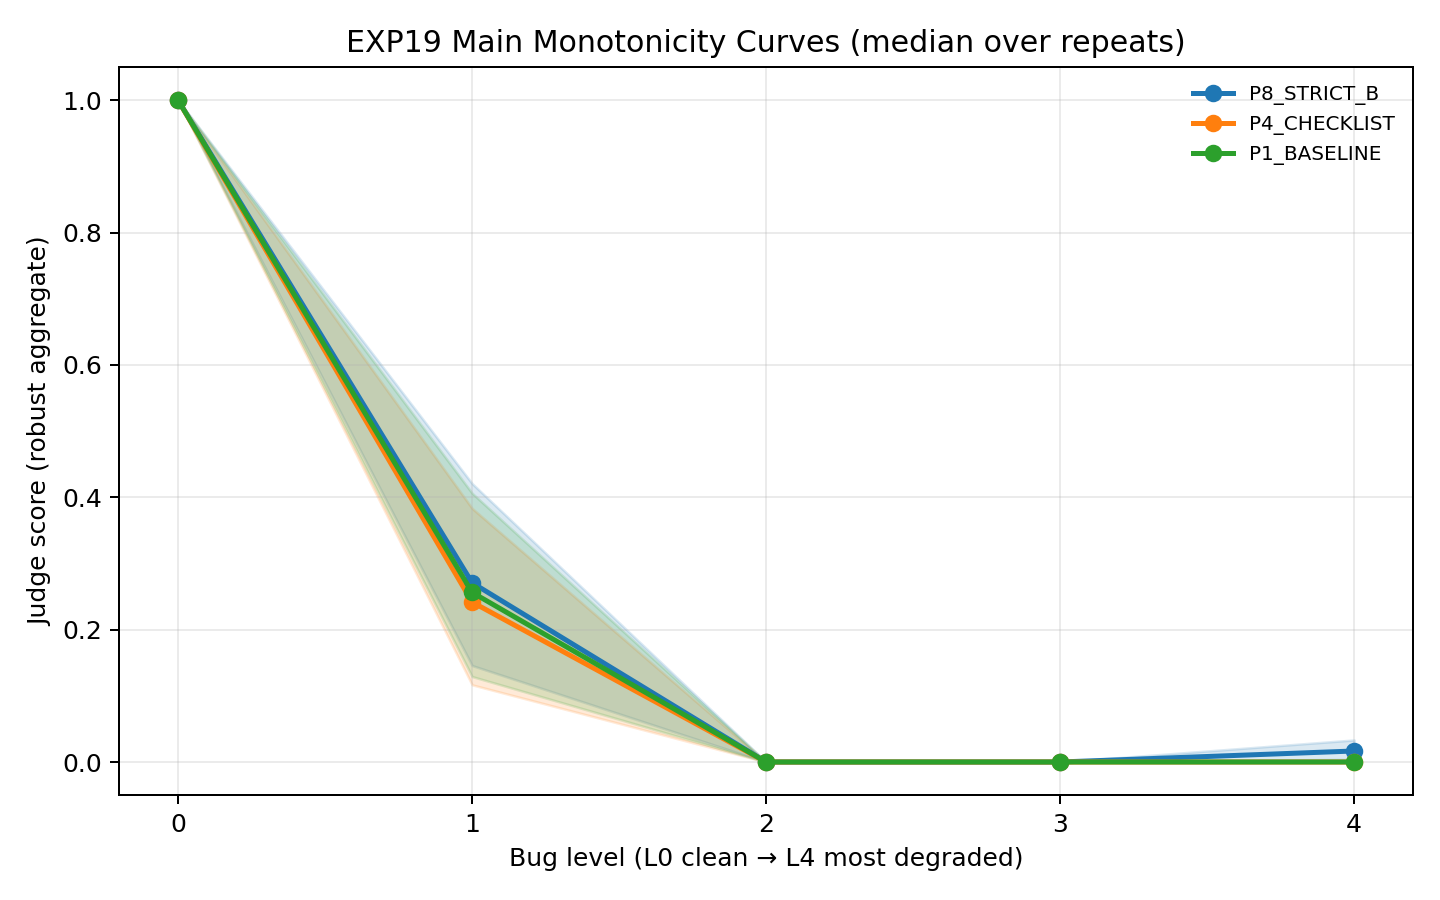
\includegraphics[width=\linewidth]{figures/fig_main_monotonicity_lowvar_exp19.png}
    \caption{Main low-variance monotonicity curves (core GPT-5.3 judges, robust repeat aggregation).}
    \label{fig:app-exp19-main-lowvar}
  \end{subfigure}\hfill
  \begin{subfigure}[t]{0.48\textwidth}
    \centering
    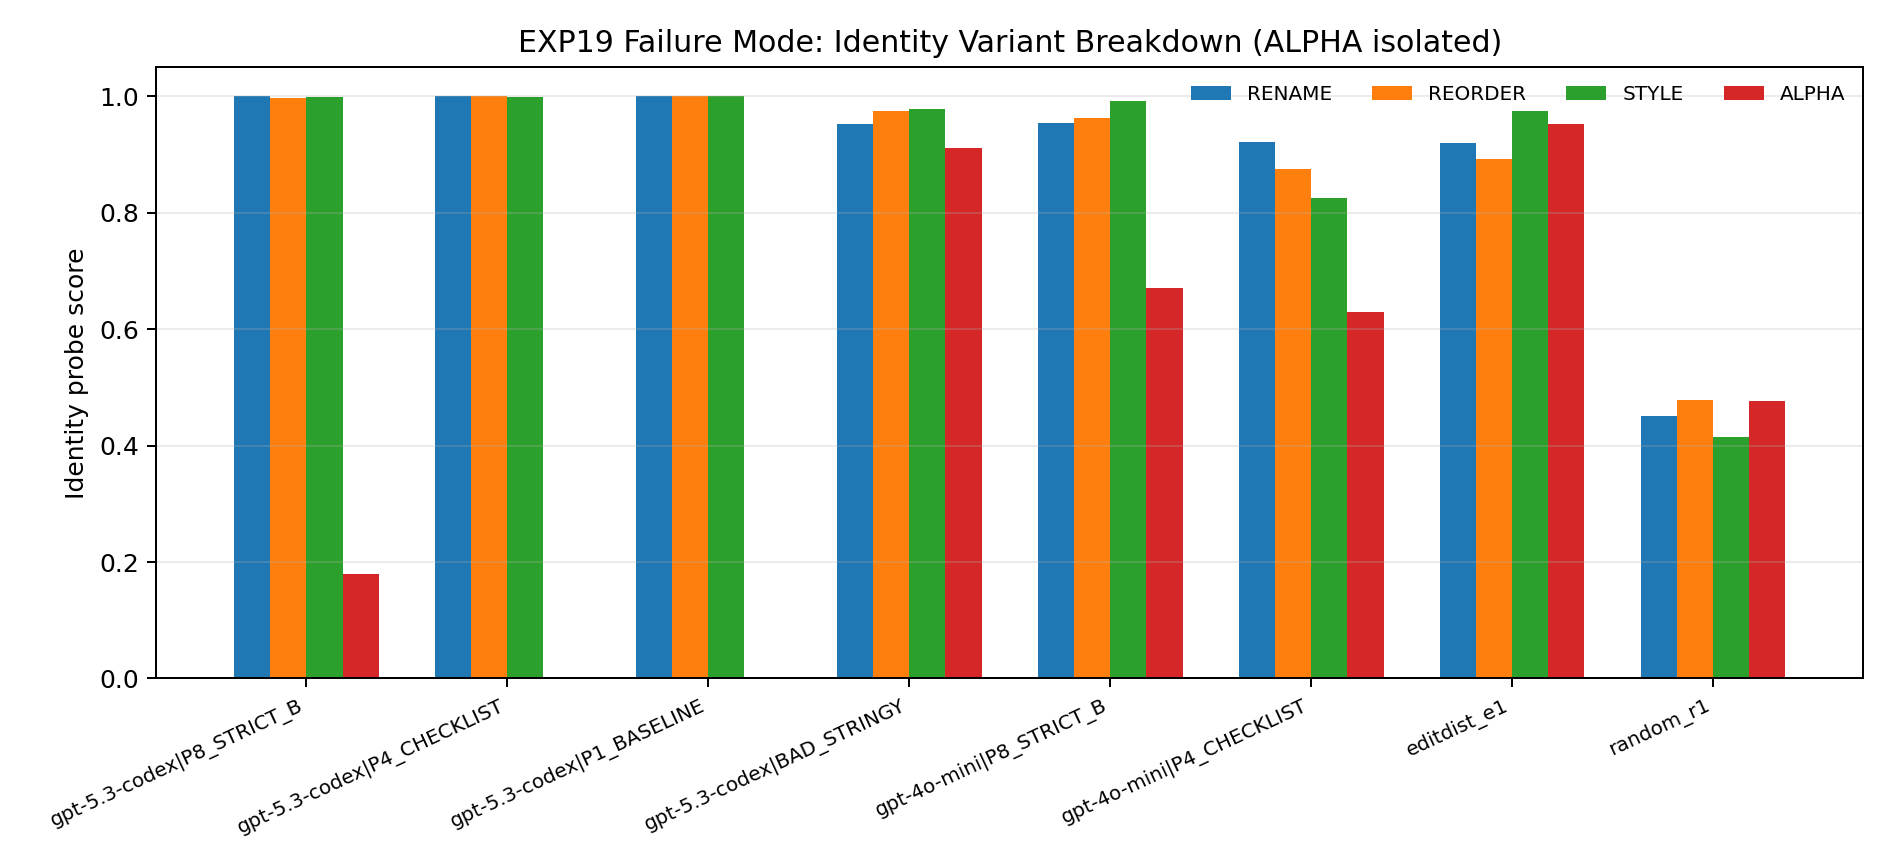
\includegraphics[width=\linewidth]{figures/fig_failure_alpha_variant_breakdown_exp19.png}
    \caption{Failure-mode isolation: identity variant breakdown with ALPHA shown separately.}
    \label{fig:app-exp19-alpha-failure}
  \end{subfigure}
  \caption{\textbf{EXP19 replot package: cleaner main trend + explicit failure separation.}
    The left panel is the ``main story'' plot with lower visual variance; the right panel isolates alpha-renaming sensitivity rather than mixing it into the primary monotonicity figure.}
  \label{fig:app-exp19-main-and-alpha}
\end{figure*}

\begin{figure}[t]
  \centering
  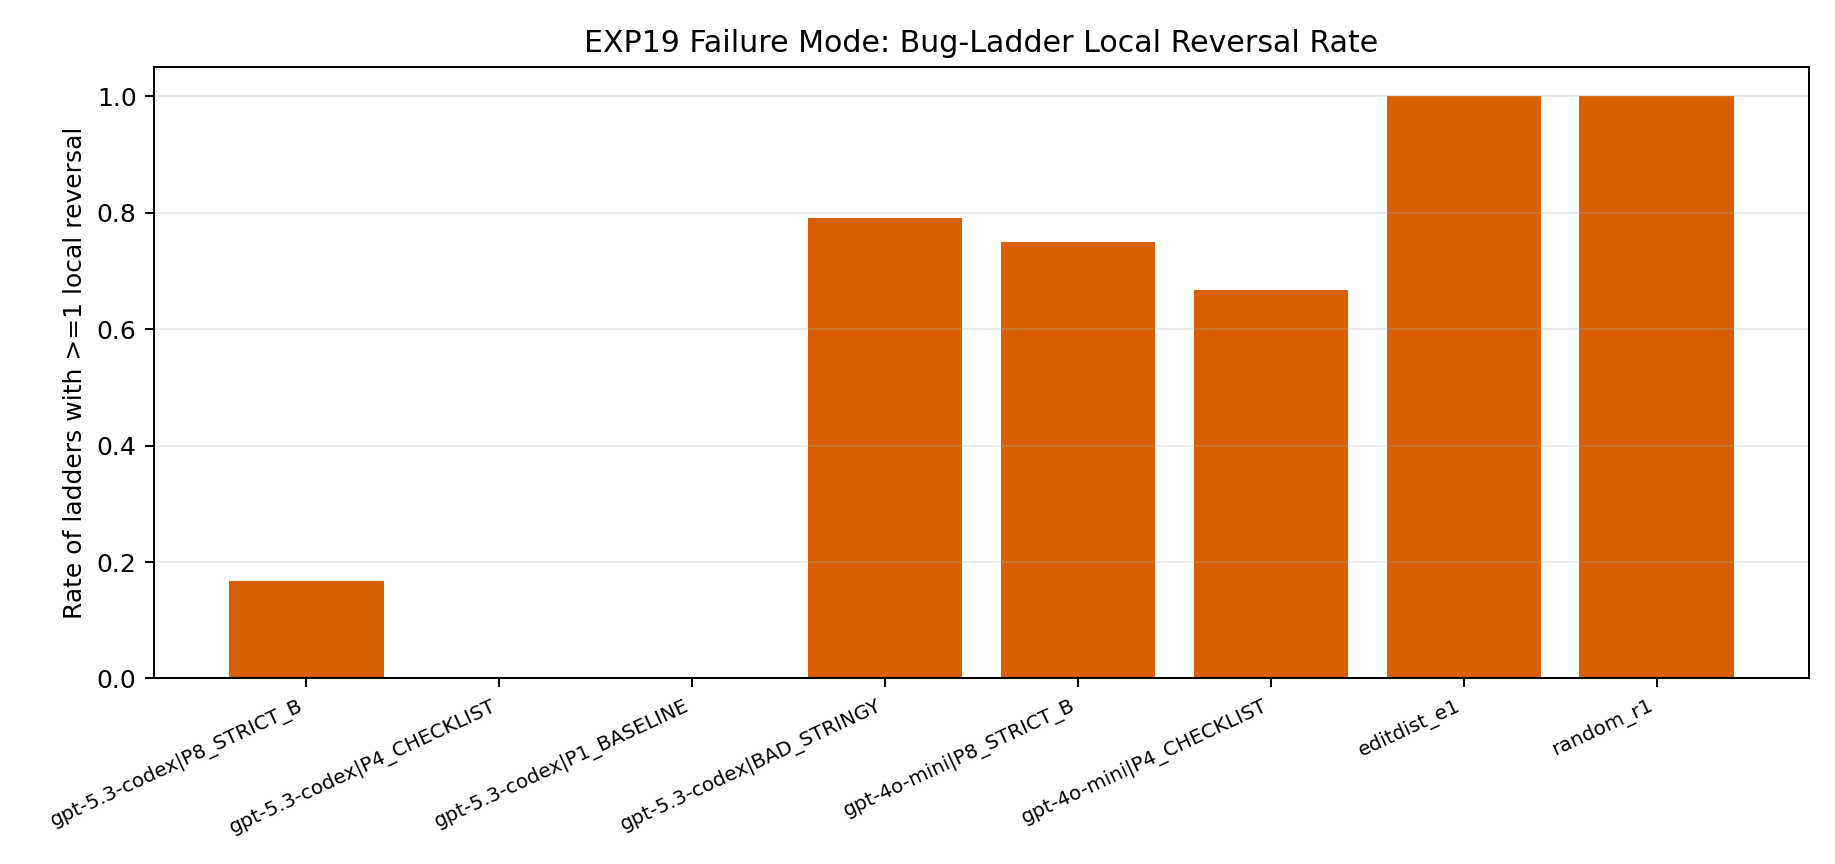
\includegraphics[width=\linewidth]{figures/fig_failure_bug_reversal_rates_exp19.png}
  \caption{\textbf{EXP19 failure-mode plot: local bug-ladder reversal rates by judge.}
    This explicitly surfaces where monotonicity fails locally, separating robustness diagnostics from the primary trend plot.}
  \label{fig:app-exp19-reversals}
\end{figure}

%%%%%%%%%%%%%%%%%%%%%%%%%%%%%%%%%%%%%%%%%%%%%%%%%%%%%%%%%%%%
\newpage
\section*{NeurIPS Paper Checklist}

\begin{enumerate}

\item {\bf Claims}
    \item[] Question: Do the main claims made in the abstract and introduction accurately reflect the paper's contributions and scope?
    \item[] Answer: \answerYes{}.
    \item[] Justification: The abstract and introduction state the judge-certification claim, the empirical setting, and the core contributions; the discussion and appendix qualify the scope and limitations.
    \item[] Guidelines:
    \begin{itemize}
        \item The answer \answerNA{} means that the abstract and introduction do not include the claims made in the paper.
        \item The abstract and/or introduction should clearly state the claims made, including the contributions made in the paper and important assumptions and limitations. A \answerNo{} or \answerNA{} answer to this question will not be perceived well by the reviewers.
        \item The claims made should match theoretical and experimental results, and reflect how much the results can be expected to generalize to other settings.
        \item It is fine to include aspirational goals as motivation as long as it is clear that these goals are not attained by the paper.
    \end{itemize}

\item {\bf Limitations}
    \item[] Question: Does the paper discuss the limitations of the work performed by the authors?
    \item[] Answer: \answerYes{}.
    \item[] Justification: The Discussion, Limitations, and appendix sections explicitly describe proxy-score limitations, finite perturbation coverage, label noise, and preliminary cross-model evidence.
    \item[] Guidelines:
    \begin{itemize}
        \item The answer \answerNA{} means that the paper has no limitation while the answer \answerNo{} means that the paper has limitations, but those are not discussed in the paper.
        \item The authors are encouraged to create a separate ``Limitations'' section in their paper.
        \item The paper should point out any strong assumptions and how robust the results are to violations of these assumptions (e.g., independence assumptions, noiseless settings, model well-specification, asymptotic approximations only holding locally). The authors should reflect on how these assumptions might be violated in practice and what the implications would be.
        \item The authors should reflect on the scope of the claims made, e.g., if the approach was only tested on a few datasets or with a few runs. In general, empirical results often depend on implicit assumptions, which should be articulated.
        \item The authors should reflect on the factors that influence the performance of the approach. For example, a facial recognition algorithm may perform poorly when image resolution is low or images are taken in low lighting. Or a speech-to-text system might not be used reliably to provide closed captions for online lectures because it fails to handle technical jargon.
        \item The authors should discuss the computational efficiency of the proposed algorithms and how they scale with dataset size.
        \item If applicable, the authors should discuss possible limitations of their approach to address problems of privacy and fairness.
        \item While the authors might fear that complete honesty about limitations might be used by reviewers as grounds for rejection, a worse outcome might be that reviewers discover limitations that aren't acknowledged in the paper. The authors should use their best judgment and recognize that individual actions in favor of transparency play an important role in developing norms that preserve the integrity of the community. Reviewers will be specifically instructed to not penalize honesty concerning limitations.
    \end{itemize}

\item {\bf Theory assumptions and proofs}
    \item[] Question: For each theoretical result, does the paper provide the full set of assumptions and a complete (and correct) proof?
    \item[] Answer: \answerNA{}.
    \item[] Justification: The paper is primarily empirical and methodological; it does not present new formal theorems requiring complete mathematical proofs.
    \item[] Guidelines:
    \begin{itemize}
        \item The answer \answerNA{} means that the paper does not include theoretical results.
        \item All the theorems, formulas, and proofs in the paper should be numbered and cross-referenced.
        \item All assumptions should be clearly stated or referenced in the statement of any theorems.
        \item The proofs can either appear in the main paper or the supplemental material, but if they appear in the supplemental material, the authors are encouraged to provide a short proof sketch to provide intuition.
        \item Inversely, any informal proof provided in the core of the paper should be complemented by formal proofs provided in appendix or supplemental material.
        \item Theorems and Lemmas that the proof relies upon should be properly referenced.
    \end{itemize}

    \item {\bf Experimental result reproducibility}
    \item[] Question: Does the paper fully disclose all the information needed to reproduce the main experimental results of the paper to the extent that it affects the main claims and/or conclusions of the paper (regardless of whether the code and data are provided or not)?
    \item[] Answer: \answerYes{}.
    \item[] Justification: The methodology and results sections report the benchmark, perturbation protocol, judge settings, repeat counts, thresholds, and bootstrap/permutation procedures used for the main claims.
    \item[] Guidelines:
    \begin{itemize}
        \item The answer \answerNA{} means that the paper does not include experiments.
        \item If the paper includes experiments, a \answerNo{} answer to this question will not be perceived well by the reviewers: Making the paper reproducible is important, regardless of whether the code and data are provided or not.
        \item If the contribution is a dataset and\slash or model, the authors should describe the steps taken to make their results reproducible or verifiable.
        \item Depending on the contribution, reproducibility can be accomplished in various ways. For example, if the contribution is a novel architecture, describing the architecture fully might suffice, or if the contribution is a specific model and empirical evaluation, it may be necessary to either make it possible for others to replicate the model with the same dataset, or provide access to the model. In general. releasing code and data is often one good way to accomplish this, but reproducibility can also be provided via detailed instructions for how to replicate the results, access to a hosted model (e.g., in the case of a large language model), releasing of a model checkpoint, or other means that are appropriate to the research performed.
        \item While NeurIPS does not require releasing code, the conference does require all submissions to provide some reasonable avenue for reproducibility, which may depend on the nature of the contribution. For example
        \begin{enumerate}
            \item If the contribution is primarily a new algorithm, the paper should make it clear how to reproduce that algorithm.
            \item If the contribution is primarily a new model architecture, the paper should describe the architecture clearly and fully.
            \item If the contribution is a new model (e.g., a large language model), then there should either be a way to access this model for reproducing the results or a way to reproduce the model (e.g., with an open-source dataset or instructions for how to construct the dataset).
            \item We recognize that reproducibility may be tricky in some cases, in which case authors are welcome to describe the particular way they provide for reproducibility. In the case of closed-source models, it may be that access to the model is limited in some way (e.g., to registered users), but it should be possible for other researchers to have some path to reproducing or verifying the results.
        \end{enumerate}
    \end{itemize}


\item {\bf Open access to data and code}
    \item[] Question: Does the paper provide open access to the data and code, with sufficient instructions to faithfully reproduce the main experimental results, as described in supplemental material?
    \item[] Answer: \answerNo{}.
    \item[] Justification: The current draft describes the evaluation protocol and cites the underlying benchmark, but it does not yet include a final anonymized code/data release URL and exact reproduction package.
    \item[] Guidelines:
    \begin{itemize}
        \item The answer \answerNA{} means that paper does not include experiments requiring code.
        \item Please see the NeurIPS code and data submission guidelines (\url{https://neurips.cc/public/guides/CodeSubmissionPolicy}) for more details.
        \item While we encourage the release of code and data, we understand that this might not be possible, so \answerNo{} is an acceptable answer. Papers cannot be rejected simply for not including code, unless this is central to the contribution (e.g., for a new open-source benchmark).
        \item The instructions should contain the exact command and environment needed to run to reproduce the results. See the NeurIPS code and data submission guidelines (\url{https://neurips.cc/public/guides/CodeSubmissionPolicy}) for more details.
        \item The authors should provide instructions on data access and preparation, including how to access the raw data, preprocessed data, intermediate data, and generated data, etc.
        \item The authors should provide scripts to reproduce all experimental results for the new proposed method and baselines. If only a subset of experiments are reproducible, they should state which ones are omitted from the script and why.
        \item At submission time, to preserve anonymity, the authors should release anonymized versions (if applicable).
        \item Providing as much information as possible in supplemental material (appended to the paper) is recommended, but including URLs to data and code is permitted.
    \end{itemize}


\item {\bf Experimental setting/details}
    \item[] Question: Does the paper specify all the training and test details (e.g., data splits, hyperparameters, how they were chosen, type of optimizer) necessary to understand the results?
    \item[] Answer: \answerYes{}.
    \item[] Justification: The paper specifies dataset splits, judge models/prompts, repeat counts, thresholds, and aggregation choices in the methodology, results, and appendix.
    \item[] Guidelines:
    \begin{itemize}
        \item The answer \answerNA{} means that the paper does not include experiments.
        \item The experimental setting should be presented in the core of the paper to a level of detail that is necessary to appreciate the results and make sense of them.
        \item The full details can be provided either with the code, in appendix, or as supplemental material.
    \end{itemize}

\item {\bf Experiment statistical significance}
    \item[] Question: Does the paper report error bars suitably and correctly defined or other appropriate information about the statistical significance of the experiments?
    \item[] Answer: \answerYes{}.
    \item[] Justification: The paper reports confidence intervals, permutation \(p\)-values, bootstrap procedures, and correlation diagnostics for the experiments supporting the main claims.
    \item[] Guidelines:
    \begin{itemize}
        \item The answer \answerNA{} means that the paper does not include experiments.
        \item The authors should answer \answerYes{} if the results are accompanied by error bars, confidence intervals, or statistical significance tests, at least for the experiments that support the main claims of the paper.
        \item The factors of variability that the error bars are capturing should be clearly stated (for example, train/test split, initialization, random drawing of some parameter, or overall run with given experimental conditions).
        \item The method for calculating the error bars should be explained (closed form formula, call to a library function, bootstrap, etc.)
        \item The assumptions made should be given (e.g., Normally distributed errors).
        \item It should be clear whether the error bar is the standard deviation or the standard error of the mean.
        \item It is OK to report 1-sigma error bars, but one should state it. The authors should preferably report a 2-sigma error bar than state that they have a 96\% CI, if the hypothesis of Normality of errors is not verified.
        \item For asymmetric distributions, the authors should be careful not to show in tables or figures symmetric error bars that would yield results that are out of range (e.g., negative error rates).
        \item If error bars are reported in tables or plots, the authors should explain in the text how they were calculated and reference the corresponding figures or tables in the text.
    \end{itemize}

\item {\bf Experiments compute resources}
    \item[] Question: For each experiment, does the paper provide sufficient information on the computer resources (type of compute workers, memory, time of execution) needed to reproduce the experiments?
    \item[] Answer: \answerNo{}.
    \item[] Justification: The draft reports experimental protocols and repeat counts, but it does not yet provide a complete hardware, memory, runtime, and total-compute accounting for every experiment.
    \item[] Guidelines:
    \begin{itemize}
        \item The answer \answerNA{} means that the paper does not include experiments.
        \item The paper should indicate the type of compute workers CPU or GPU, internal cluster, or cloud provider, including relevant memory and storage.
        \item The paper should provide the amount of compute required for each of the individual experimental runs as well as estimate the total compute.
        \item The paper should disclose whether the full research project required more compute than the experiments reported in the paper (e.g., preliminary or failed experiments that didn't make it into the paper).
    \end{itemize}

\item {\bf Code of ethics}
    \item[] Question: Does the research conducted in the paper conform, in every respect, with the NeurIPS Code of Ethics \url{https://neurips.cc/public/EthicsGuidelines}?
    \item[] Answer: \answerYes{}.
    \item[] Justification: The work evaluates formal-verification artifacts and LLM judges, reports limitations and failure modes, and does not rely on private or personally identifying data.
    \item[] Guidelines:
    \begin{itemize}
        \item The answer \answerNA{} means that the authors have not reviewed the NeurIPS Code of Ethics.
        \item If the authors answer \answerNo, they should explain the special circumstances that require a deviation from the Code of Ethics.
        \item The authors should make sure to preserve anonymity (e.g., if there is a special consideration due to laws or regulations in their jurisdiction).
    \end{itemize}


\item {\bf Broader impacts}
    \item[] Question: Does the paper discuss both potential positive societal impacts and negative societal impacts of the work performed?
    \item[] Answer: \answerYes{}.
    \item[] Justification: The discussion frames positive impacts for scalable oversight and formal verification, and it also describes risks from proxy judging, prompt sensitivity, and incomplete gold specifications.
    \item[] Guidelines:
    \begin{itemize}
        \item The answer \answerNA{} means that there is no societal impact of the work performed.
        \item If the authors answer \answerNA{} or \answerNo, they should explain why their work has no societal impact or why the paper does not address societal impact.
        \item Examples of negative societal impacts include potential malicious or unintended uses (e.g., disinformation, generating fake profiles, surveillance), fairness considerations (e.g., deployment of technologies that could make decisions that unfairly impact specific groups), privacy considerations, and security considerations.
        \item The conference expects that many papers will be foundational research and not tied to particular applications, let alone deployments. However, if there is a direct path to any negative applications, the authors should point it out. For example, it is legitimate to point out that an improvement in the quality of generative models could be used to generate Deepfakes for disinformation. On the other hand, it is not needed to point out that a generic algorithm for optimizing neural networks could enable people to train models that generate Deepfakes faster.
        \item The authors should consider possible harms that could arise when the technology is being used as intended and functioning correctly, harms that could arise when the technology is being used as intended but gives incorrect results, and harms following from (intentional or unintentional) misuse of the technology.
        \item If there are negative societal impacts, the authors could also discuss possible mitigation strategies (e.g., gated release of models, providing defenses in addition to attacks, mechanisms for monitoring misuse, mechanisms to monitor how a system learns from feedback over time, improving the efficiency and accessibility of ML).
    \end{itemize}

\item {\bf Safeguards}
    \item[] Question: Does the paper describe safeguards that have been put in place for responsible release of data or models that have a high risk for misuse (e.g., pre-trained language models, image generators, or scraped datasets)?
    \item[] Answer: \answerNA{}.
    \item[] Justification: The paper does not release a new high-risk model, scraped dataset, or dual-use generative model requiring release safeguards.
    \item[] Guidelines:
    \begin{itemize}
        \item The answer \answerNA{} means that the paper poses no such risks.
        \item Released models that have a high risk for misuse or dual-use should be released with necessary safeguards to allow for controlled use of the model, for example by requiring that users adhere to usage guidelines or restrictions to access the model or implementing safety filters.
        \item Datasets that have been scraped from the Internet could pose safety risks. The authors should describe how they avoided releasing unsafe images.
        \item We recognize that providing effective safeguards is challenging, and many papers do not require this, but we encourage authors to take this into account and make a best faith effort.
    \end{itemize}

\item {\bf Licenses for existing assets}
    \item[] Question: Are the creators or original owners of assets (e.g., code, data, models), used in the paper, properly credited and are the license and terms of use explicitly mentioned and properly respected?
    \item[] Answer: \answerNo{}.
    \item[] Justification: Existing benchmarks and related assets are cited, but the current draft does not yet enumerate all license terms and asset-use conditions.
    \item[] Guidelines:
    \begin{itemize}
        \item The answer \answerNA{} means that the paper does not use existing assets.
        \item The authors should cite the original paper that produced the code package or dataset.
        \item The authors should state which version of the asset is used and, if possible, include a URL.
        \item The name of the license (e.g., CC-BY 4.0) should be included for each asset.
        \item For scraped data from a particular source (e.g., website), the copyright and terms of service of that source should be provided.
        \item If assets are released, the license, copyright information, and terms of use in the package should be provided. For popular datasets, \url{paperswithcode.com/datasets} has curated licenses for some datasets. Their licensing guide can help determine the license of a dataset.
        \item For existing datasets that are re-packaged, both the original license and the license of the derived asset (if it has changed) should be provided.
        \item If this information is not available online, the authors are encouraged to reach out to the asset's creators.
    \end{itemize}

\item {\bf New assets}
    \item[] Question: Are new assets introduced in the paper well documented and is the documentation provided alongside the assets?
    \item[] Answer: \answerNA{}.
    \item[] Justification: The submission introduces an evaluation methodology and reports experiments, but it does not claim release of a new dataset or model asset in the current draft.
    \item[] Guidelines:
    \begin{itemize}
        \item The answer \answerNA{} means that the paper does not release new assets.
        \item Researchers should communicate the details of the dataset\slash code\slash model as part of their submissions via structured templates. This includes details about training, license, limitations, etc.
        \item The paper should discuss whether and how consent was obtained from people whose asset is used.
        \item At submission time, remember to anonymize your assets (if applicable). You can either create an anonymized URL or include an anonymized zip file.
    \end{itemize}

\item {\bf Crowdsourcing and research with human subjects}
    \item[] Question: For crowdsourcing experiments and research with human subjects, does the paper include the full text of instructions given to participants and screenshots, if applicable, as well as details about compensation (if any)?
    \item[] Answer: \answerNA{}.
    \item[] Justification: The reported human labels are used as evaluation labels for judge alignment, but the draft does not describe a crowdsourcing study or recruited human-subject experiment.
    \item[] Guidelines:
    \begin{itemize}
        \item The answer \answerNA{} means that the paper does not involve crowdsourcing nor research with human subjects.
        \item Including this information in the supplemental material is fine, but if the main contribution of the paper involves human subjects, then as much detail as possible should be included in the main paper.
        \item According to the NeurIPS Code of Ethics, workers involved in data collection, curation, or other labor should be paid at least the minimum wage in the country of the data collector.
    \end{itemize}

\item {\bf Institutional review board (IRB) approvals or equivalent for research with human subjects}
    \item[] Question: Does the paper describe potential risks incurred by study participants, whether such risks were disclosed to the subjects, and whether Institutional Review Board (IRB) approvals (or an equivalent approval/review based on the requirements of your country or institution) were obtained?
    \item[] Answer: \answerNA{}.
    \item[] Justification: The paper does not report a crowdsourcing or human-subject study requiring IRB-style approval.
    \item[] Guidelines:
    \begin{itemize}
        \item The answer \answerNA{} means that the paper does not involve crowdsourcing nor research with human subjects.
        \item Depending on the country in which research is conducted, IRB approval (or equivalent) may be required for any human subjects research. If you obtained IRB approval, you should clearly state this in the paper.
        \item We recognize that the procedures for this may vary significantly between institutions and locations, and we expect authors to adhere to the NeurIPS Code of Ethics and the guidelines for their institution.
        \item For initial submissions, do not include any information that would break anonymity (if applicable), such as the institution conducting the review.
    \end{itemize}

\item {\bf Declaration of LLM usage}
    \item[] Question: Does the paper describe the usage of LLMs if it is an important, original, or non-standard component of the core methods in this research? Note that if the LLM is used only for writing, editing, or formatting purposes and does \emph{not} impact the core methodology, scientific rigor, or originality of the research, declaration is not required.
    %this research?
    \item[] Answer: \answerYes{}.
    \item[] Justification: LLMs are a core component of the proposed judge and certification experiments, and the paper explicitly describes the LLM-judge setup, prompts, repeats, and model families.
    \item[] Guidelines:
    \begin{itemize}
        \item The answer \answerNA{} means that the core method development in this research does not involve LLMs as any important, original, or non-standard components.
        \item Please refer to our LLM policy in the NeurIPS handbook for what should or should not be described.
    \end{itemize}

\end{enumerate}


\end{document}
